%==============================================================================
% tento soubor pouzijte jako zaklad
% this file should be used as a base for the thesis
% Autoři / Authors: 2008 Michal Bidlo, 2019 Jaroslav Dytrych
% Kontakt pro dotazy a připomínky: sablona@fit.vutbr.cz
% Contact for questions and comments: sablona@fit.vutbr.cz
%==============================================================================
% kodovani: UTF-8 (zmena prikazem iconv, recode nebo cstocs)
% encoding: UTF-8 (you can change it by command iconv, recode or cstocs)
%------------------------------------------------------------------------------
% zpracování / processing: make, make pdf, make clean
%==============================================================================
% Soubory, které je nutné upravit nebo smazat: / Files which have to be edited or deleted:
%   projekt-20-literatura-bibliography.bib - literatura / bibliography
%   projekt-01-kapitoly-chapters.tex - obsah práce / the thesis content
%   projekt-01-kapitoly-chapters-en.tex - obsah práce v angličtině / the thesis content in English
%   projekt-30-prilohy-appendices.tex - přílohy / appendices
%   projekt-30-prilohy-appendices-en.tex - přílohy v angličtině / appendices in English
%==============================================================================
% \documentclass[]{fitthesis} % bez zadání - pro začátek práce, aby nebyl problém s překladem
%\documentclass[english]{fitthesis} % without assignment - for the work start to avoid compilation problem
\documentclass[zadani]{fitthesis} % odevzdani do wisu a/nebo tisk s barevnými odkazy - odkazy jsou barevné
%\documentclass[english,zadani]{fitthesis} % for submission to the IS FIT and/or print with color links - links are color
%\documentclass[zadani,print]{fitthesis} % pro černobílý tisk - odkazy jsou černé
%\documentclass[english,zadani,print]{fitthesis} % for the black and white print - links are black
%\documentclass[zadani,cprint]{fitthesis} % pro barevný tisk - odkazy jsou černé, znak VUT barevný
%\documentclass[english,zadani,cprint]{fitthesis} % for the print - links are black, logo is color
% * Je-li práce psaná v anglickém jazyce, je zapotřebí u třídy použít 
%   parametr english následovně:
%   If thesis is written in English, it is necessary to use 
%   parameter english as follows:
%      \documentclass[english]{fitthesis}
% * Je-li práce psaná ve slovenském jazyce, je zapotřebí u třídy použít 
%   parametr slovak následovně:
%   If the work is written in the Slovak language, it is necessary 
%   to use parameter slovak as follows:
%      \documentclass[slovak]{fitthesis}
% * Je-li práce psaná v anglickém jazyce se slovenským abstraktem apod., 
%   je zapotřebí u třídy použít parametry english a enslovak následovně:
%   If the work is written in English with the Slovak abstract, etc., 
%   it is necessary to use parameters english and enslovak as follows:
%      \documentclass[english,enslovak]{fitthesis}

% Základní balíčky jsou dole v souboru šablony fitthesis.cls
% Basic packages are at the bottom of template file fitthesis.cls
% zde můžeme vložit vlastní balíčky / you can place own packages here

% Kompilace po částech (rychlejší, ale v náhledu nemusí být vše aktuální)
% Compilation piecewise (faster, but not all parts in preview will be up-to-date)
% \usepackage{subfiles}

% Nastavení cesty k obrázkům
% Setting of a path to the pictures
%\graphicspath{{obrazky-figures/}{./obrazky-figures/}}
%\graphicspath{{obrazky-figures/}{../obrazky-figures/}}

%---rm---------------
\renewcommand{\rmdefault}{lmr}%zavede Latin Modern Roman jako rm / set Latin Modern Roman as rm
%---sf---------------
\renewcommand{\sfdefault}{qhv}%zavede TeX Gyre Heros jako sf
%---tt------------
\renewcommand{\ttdefault}{lmtt}% zavede Latin Modern tt jako tt

% vypne funkci šablony, která automaticky nahrazuje uvozovky,
% aby nebyly prováděny nevhodné náhrady v popisech API apod.
% disables function of the template which replaces quotation marks
% to avoid unnecessary replacements in the API descriptions etc.
\csdoublequotesoff

\usepackage{minted}
\usepackage{float}
\usepackage{url}
\usepackage{mymacros}
\usepackage{subcaption}
\usepackage{adjustbox}
\usepackage{makecell}


% =======================================================================
% balíček "hyperref" vytváří klikací odkazy v pdf, pokud tedy použijeme pdflatex
% problém je, že balíček hyperref musí být uveden jako poslední, takže nemůže
% být v šabloně
% "hyperref" package create clickable links in pdf if you are using pdflatex.
% Problem is that this package have to be introduced as the last one so it 
% can not be placed in the template file.
\ifWis
\ifx\pdfoutput\undefined % nejedeme pod pdflatexem / we are not using pdflatex
\else
  \usepackage{color}
  \usepackage[unicode,colorlinks,hyperindex,plainpages=false,pdftex]{hyperref}
  \definecolor{hrcolor-ref}{RGB}{223,52,30}
  \definecolor{hrcolor-cite}{HTML}{2F8F00}
  \definecolor{hrcolor-urls}{HTML}{092EAB}
  \hypersetup{
	linkcolor=hrcolor-ref,
	citecolor=hrcolor-cite,
	filecolor=magenta,
	urlcolor=hrcolor-urls
  }
  \def\pdfBorderAttrs{/Border [0 0 0] }  % bez okrajů kolem odkazů / without margins around links
  \pdfcompresslevel=9
\fi
\else % pro tisk budou odkazy, na které se dá klikat, černé / for the print clickable links will be black
\ifx\pdfoutput\undefined % nejedeme pod pdflatexem / we are not using pdflatex
\else
  \usepackage{color}
  \usepackage[unicode,colorlinks,hyperindex,plainpages=false,pdftex,urlcolor=black,linkcolor=black,citecolor=black]{hyperref}
  \definecolor{links}{rgb}{0,0,0}
  \definecolor{anchors}{rgb}{0,0,0}
  \def\AnchorColor{anchors}
  \def\LinkColor{links}
  \def\pdfBorderAttrs{/Border [0 0 0] } % bez okrajů kolem odkazů / without margins around links
  \pdfcompresslevel=9
\fi
\fi
% Řešení problému, kdy klikací odkazy na obrázky vedou za obrázek
% This solves the problems with links which leads after the picture
\usepackage[all]{hypcap}

% Informace o práci/projektu / Information about the thesis
%---------------------------------------------------------------------------
\projectinfo{
  %Prace / Thesis
  project={BP},            %typ práce BP/SP/DP/DR  / thesis type (SP = term project)
  year={2021},             % rok odevzdání / year of submission
  date=\today,             % datum odevzdání / submission date
  %Nazev prace / thesis title
  title.cs={Analýza audio hovoru mezi dvěma účastníky},  % název práce v češtině či slovenštině (dle zadání) / thesis title in czech language (according to assignment)
  title.en={Interview Analysis}, % název práce v angličtině / thesis title in english
  title.length={14cm}, % nastavení délky bloku s titulkem pro úpravu zalomení řádku (lze definovat zde nebo níže) / setting the length of a block with a thesis title for adjusting a line break (can be defined here or below)
  %sectitle.length={14.5cm}, % nastavení délky bloku s druhým titulkem pro úpravu zalomení řádku (lze definovat zde nebo níže) / setting the length of a block with a second thesis title for adjusting a line break (can be defined here or below)
  %Autor / Author
  author.name={Alexander},   % jméno autora / author name
  author.surname={Polok},   % příjmení autora / author surname 
  %author.title.p={Bc.}, % titul před jménem (nepovinné) / title before the name (optional)
  %author.title.a={Ph.D.}, % titul za jménem (nepovinné) / title after the name (optional)
  %Ustav / Department
  department={UPGM}, % doplňte příslušnou zkratku dle ústavu na zadání: UPSY/UIFS/UITS/UPGM / fill in appropriate abbreviation of the department according to assignment: UPSY/UIFS/UITS/UPGM
  % Školitel / supervisor
  supervisor.name={Pavel},   % jméno školitele / supervisor name 
  supervisor.surname={Matějka},   % příjmení školitele / supervisor surname
  supervisor.title.p={Ing.},   %titul před jménem (nepovinné) / title before the name (optional)
  supervisor.title.a={Ph.D.},    %titul za jménem (nepovinné) / title after the name (optional)
  % Klíčová slova / keywords
  keywords.cs={Analýza rozhovoru, Online psychoterapie, Klient a terapeut, Zpětná vazba, Detekce řečové aktivity, Diarizace, Zpracování řeči, Zpracování přirozeného jazyka, Paralingvistika}, % klíčová slova v českém či slovenském jazyce / keywords in czech or slovak language
  keywords.en={Conversation analysis, Online psychotherapy, Client and therapist, Feedback, Speech activity detection, Diarization, Speech processing, Natural language processing, Paralinguistics}, % klíčová slova v anglickém jazyce / keywords in english
  %keywords.en={Here, individual keywords separated by commas will be written in English.},
  % Abstrakt / Abstract
  abstract.cs={Cílem této práce je analýza psychoterapeutických sezení. Z audionahrávek jsou extrahovány klasifikátory, které popisují proběhlou terapii. Ty jsou následně agregovány, porovnány s ostatními sezeními a graficky prezentovány v podobě zprávy shrnující daný rozhovor. Terapeutům je tímto způsobem k proběhlým sezením poskytnuta zpětná vazba, která může sloužit k profesnímu růstu a kvalitnější psychoterapii v budoucnu.}, % abstrakt v českém či slovenském jazyce / abstract in czech or slovak language
  abstract.en={The aim of this thesis is the analysis of psychotherapeutic sessions. Classifiers describing the therapy are extracted from the audio recordings. These are then aggregated, compared with other sessions, and graphically presented in a report summarizing the conversation. In this way, therapists are provided with feedback that can serve for professional growth and better psychotherapy in the future.}, % abstrakt v anglickém jazyce / abstract in english
  %abstract.en={An abstract of the work in English will be written in this paragraph.},
  % Prohlášení (u anglicky psané práce anglicky, u slovensky psané práce slovensky) / Declaration (for thesis in english should be in english)
  declaration={Prohlašuji, že jsem tuto bakalářskou práci vypracoval samostatně pod vedením pana Ing. Pavla Matějky, Ph.D. Uvedl jsem všechny literární prameny, publikace a další zdroje, ze kterých jsem čerpal.},
  %declaration={I hereby declare that this Bachelor's thesis was prepared as an original work by the author under the supervision of Mr. X
% The supplementary information was provided by Mr. Y
% I have listed all the literary sources, publications and other sources, which were used during the preparation of this thesis.},
  % Poděkování (nepovinné, nejlépe v jazyce práce) / Acknowledgement (optional, ideally in the language of the thesis)
  acknowledgment={Chtěl bych poděkovat vedoucímu práce, Ing. Pavlovi Matějkovi, Ph.D., za všechen čas, který byl ochoten věnovat konzultacím, za pomoc při řešení nejrůznějších problémů a za velmi přátelský a vstřícný přístup.
  
  Zároveň bych chtěl poděkovat paní Drahomíře Šloufové, Michalu Rozsívalovi a moji skvělé přítelkyni za korekturu gramatických chyb. Speciální poděkování patří Ladislavu Ondrisovi, s nimž jsem celou práci průběžně diskutoval a poskytl mi mnoho cenných rad a podnětů ke zlepšení.},
  %acknowledgment={Here it is possible to express thanks to the supervisor and to the people which provided professional help
%(external submitter, consultant, etc.).},
  % Rozšířený abstrakt (cca 3 normostrany) - lze definovat zde nebo níže / Extended abstract (approximately 3 standard pages) - can be defined here or below
  %extendedabstract={Do tohoto odstavce bude zapsán rozšířený výtah (abstrakt) práce v českém (slovenském) jazyce.},
  %faculty={FIT}, % FIT/FEKT/FSI/FA/FCH/FP/FAST/FAVU/USI/DEF
  faculty.cs={Fakulta informačních technologií}, % Fakulta v češtině - pro využití této položky výše zvolte fakultu DEF / Faculty in Czech - for use of this entry select DEF above
  faculty.en={Faculty of Information Technology}, % Fakulta v angličtině - pro využití této položky výše zvolte fakultu DEF / Faculty in English - for use of this entry select DEF above
  department.cs={Ústav matematiky}, % Ústav v češtině - pro využití této položky výše zvolte ústav DEF nebo jej zakomentujte / Department in Czech - for use of this entry select DEF above or comment it out
  department.en={Institute of Mathematics} % Ústav v angličtině - pro využití této položky výše zvolte ústav DEF nebo jej zakomentujte / Department in English - for use of this entry select DEF above or comment it out
}

% Rozšířený abstrakt (cca 3 normostrany) - lze definovat zde nebo výše / Extended abstract (approximately 3 standard pages) - can be defined here or above
%\extendedabstract{Do tohoto odstavce bude zapsán výtah (abstrakt) práce v českém (slovenském) jazyce.}

% nastavení délky bloku s titulkem pro úpravu zalomení řádku - lze definovat zde nebo výše / setting the length of a block with a thesis title for adjusting a line break - can be defined here or above
%\titlelength{14.5cm}
% nastavení délky bloku s druhým titulkem pro úpravu zalomení řádku - lze definovat zde nebo výše / setting the length of a block with a second thesis title for adjusting a line break - can be defined here or above
%\sectitlelength{14.5cm}

% řeší první/poslední řádek odstavce na předchozí/následující stránce
% solves first/last row of the paragraph on the previous/next page
\clubpenalty=10000
\widowpenalty=10000

% checklist
\newlist{checklist}{itemize}{1}
\setlist[checklist]{label=$\square$}

\begin{document}
  % Vysazeni titulnich stran / Typesetting of the title pages
  % ----------------------------------------------
  \maketitle
  % Obsah
  % ----------------------------------------------
  \setlength{\parskip}{0pt}

  \setcounter{tocdepth}{1} % v Obsahu jsou pouze kapitoly do druhé úrovně -- takto je to správně
  {\hypersetup{hidelinks}\tableofcontents}
  
  % Seznam obrazku a tabulek (pokud prace obsahuje velke mnozstvi obrazku, tak se to hodi)
  % List of figures and list of tables (if the thesis contains a lot of pictures, it is good)
  \ifczech
    \renewcommand\listfigurename{Seznam obrázků}
  \fi
  \ifslovak
    \renewcommand\listfigurename{Zoznam obrázkov}
  \fi
  % {\hypersetup{hidelinks}\listoffigures}
  
  \ifczech
    \renewcommand\listtablename{Seznam tabulek}
  \fi
  \ifslovak
    \renewcommand\listtablename{Zoznam tabuliek}
  \fi
  % {\hypersetup{hidelinks}\listoftables}

  \ifODSAZ
    \setlength{\parskip}{0.5\bigskipamount}
  \else
    \setlength{\parskip}{0pt}
  \fi

  % vynechani stranky v oboustrannem rezimu
  % Skip the page in the two-sided mode
  \iftwoside
    \cleardoublepage
  \fi

  % Text prace / Thesis text
  % ----------------------------------------------
  \ifenglish
    \input{projekt-kapitoly-chapters-en}
  \else
    %%%%%%%%%%%%%%%%%%%%%%%%%%%%% Úvod %%%%%%%%%%%%%%%%%%%%%%%%%%%%%
\chapter{Úvod}
Zpracování řeči a její analýza je v~dnešní době celosvětově velmi rozvíjený a diskutovaný obor. Existuje nespočet odborných skupin věnujících se problematice identifikace řečníka, identifikaci jazyka, rozpoznávání řeči, detekci klíčových slov, rozpoznávání fonémů nebo zpracování přirozeného jazyka. Technologický rozvoj v~posledních letech způsobil, že systémy věnující se problematice zpracování řeči dosahují velmi vysokých přesností a můžeme se s~nimi setkat skoro na denní bázi, ať už třeba v~podobě virtuálních asistentů Siri, Alexa nebo v~rámci zlepšování kvality call center. Tato práce se zaměřuje na analýzu psychoterapeutického sezení. Psychoterapie je původem latinské slovo -- skládající se z~části psyché (výrazu pro lidskou duši či mysl) a therapeia (léčba). Jejím cílem je léčit mysl, obnovit její rovnováhu a vést ke zkvalitnění života klienta.

Pandemie virové choroby covid-19 změnila životy mnohých a zvýšila taktéž poptávku po psychoterapeutických sezeních, ať už z~důvodu chybějící sociální interakce nebo zvýšeného stresu a nejistoty. Se zvyšující se poptávkou po psychoterapii a snahou o~zamezení šíření choroby, což se projevilo v~podobě mnoha vládních opatření, mezi něž patří především omezení kontaktu, se rozšířila alternativa známá jako online psychoterapie. Terapie pomocí video hovoru nebyla dosud v~České republice příliš známá. Ve Spojených státech amerických, v~severní Evropě nebo Velké Británii je však tato forma běžná a je často jedinou formou pomoci, kterou mohou využít invalidé, nemocní a lidé bydlící v~odlehlých oblastech. 

Forma video hovoru přináší možnost analyzovat psychoterapeutické sezení strojově a získat tímto způsobem nové informace o~proběhlém sezení. Cílem není hodnotit úspěšnost terapie, ale nalézt klasifikátory a časové úseky, které dokážou terapeuta upozornit například na vyšší výskyt skákání do řeči nebo výskyt změny emočního stavu klienta. 

Kapitola~\ref{chap:FeatureExctraction} se zaměřuje na objasnění použitých technik. V~rámci kapitoly~\ref{chap:Data} jsou představena data, pro jejichž zpracování byl systém navržen. Detaily návrhu tohoto systému jsou popsány v~kapitole~\ref{chap:System_design}, v~rámci této kapitoly jsou rovněž představeny klasifikátory obsažené ve výsledné souhrnné zprávě. Souhrnná zpráva, jež je výstupem této práce, může částečně nahrazovat drahou supervizi u~mladých psychoterapeutů, kteří ukončili vzdělání a získávají praxi. Dokument přináší porovnání s~ostatními terapeuty. Pro příslušné druhy terapie se však mohou metriky velmi lišit a interpretace hodnot už je na samotném terapeutovi, případně jeho zkušenějším kolegovi.

Kapitola~\ref{chap:Implementation} přibližuje implementační detaily navrženého systému. Obsahuje informace o~použitých technologiích, algoritmech, knihovnách a externích nástrojích. V~kapitole~\ref{chap:Evaluation} jsou popsány experimenty, které vedly ke zlepšení přesnosti navrženého systému.
V~kapitole \ref{chap:Conclusion} jsou sumarizovány výsledky této práce a navržen další postup.

%%%%%%%%%%%%%%%%%%%%%%%%%%%%% Teorie %%%%%%%%%%%%%%%%%%%%%%%%%%%%%


\chapter{Analýza audio nahrávky a extrakce příznaků}
\label{chap:FeatureExctraction}
V~rámci této kapitoly je čtenář uveden do problematiky zpracování řečových signálů. Je mu postupně představen celý proces od zaznamenání vibrací vzduchu reprezentujících zvuk, až po metody použité pro rozpoznání řeči příslušných mluvčích. \imageref{fig:ProcessingSchema}{1} demonstruje celý proces analýzy audio nahrávek klienta a terapeuta. Extrakcí statistik a tvorbou souhrnné zprávy se blíže zabývá kapitola~\ref{chap:System_design}.

\begin{figure}[ht]
  \centering
  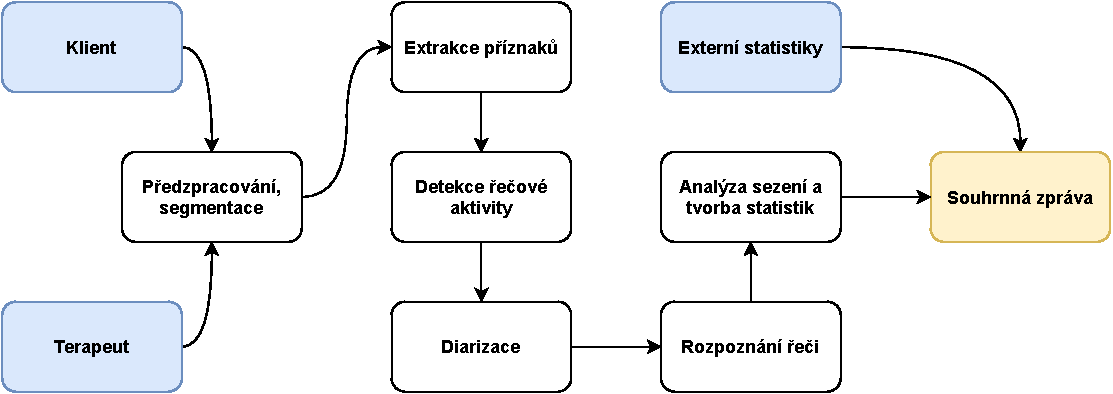
\includegraphics[width=\linewidth]{obrazky-figures/schema.pdf}
  \caption{Proces zpracování vstupních nahrávek terapeuta a klienta. Prvním krokem analýzy je segmentace zvukové nahrávky. Ze segmentů jsou extrahovány příznaky, s~jejichž pomocí dochází k~určení řečově aktivních segmentů příslušných řečníků. Následně je vytvořen přepis z~těchto řečově aktivní segmentů. Na závěr jsou vypočteny statistiky o~sezení a je vytvořena souhrnná zpráva zahrnující porovnání s~ostatními sezeními.}
  \label{fig:ProcessingSchema}
\end{figure}

%%%%%%%%%%%%%%%%%%%%%%%%%%%%%%


\section{Řečový signál}
\label{section:Speech_signal}
Schopnost vyjadřovat se a rozumět mluvené řeči je dána pouze lidskému druhu jako doposud jedinému známému organismus žijícímu na Zemi. Občas sice říkáme, že mluví i papoušci, jedná se však jen o~zvukové napodobení tvořené zcela jiným způsobem, než je artikulovaná řeč člověka. Zvuková řeč má významné postavení ve vývoji člověka jako druhu. Řeč je řízená mozkem a to zejména mozkovým centrem mluvení (řečového výkonu -- centrum Wernickovo) a centrem slyšení řeči (dešifrování slyšeného signálu -- centrum Brockovo). Důsledkem poškození mozku mohou vzniknout poruchy, které řeč postihují. Mezi nejznámější patří afázie (neschopnost řeč tvořit nebo ji porozumět), koktavost, breptavost, řidčeji se může objevit oněmění, ev. mluvní negativismus~\cite{Fonetika_Krcmova}.

Princip tvorby řeči, který je velmi podobný vytváření tónu u~dechových nástrojů, je znázorněn na~\imageref{fig:VoiceCreationSchema}{}. Samotná řeč vzniká proudem vzduchu, který je dodáván plícemi. Takto vzniklý proud prochází hlasivkovou štěrbinou, která je obklopena kmitajícími hlasivkami tvořícími budící signál. Tento signál však ještě nepovažujeme za řeč. Až artikulací, tedy příslušnou konfigurací řečových orgánů v~dutině hrdelní, ústní a nosní, dochází ke vzniku zopakovatelných úseků řeči -- hlásek~\cite{Sigmund_Analyza}.

\begin{figure}[ht]
  \centering
  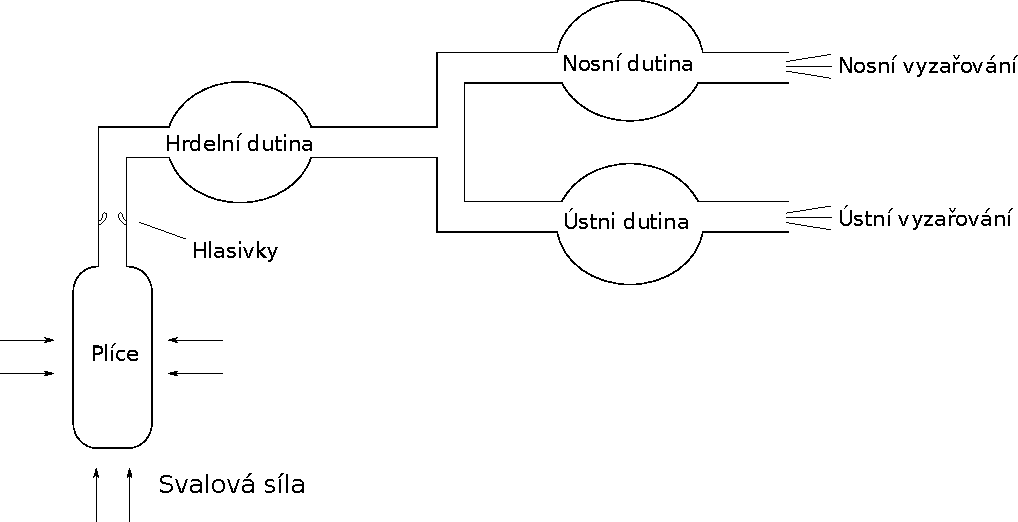
\includegraphics[width=\linewidth]{obrazky-figures/vocal_tract.pdf}
  \caption{Schematické znázornění hlasového ústroji.}
  \label{fig:VoiceCreationSchema}
\end{figure}

Řeč je možné prezentovat jako soubor informací nebo jako fyzikální signál, který přenáší nejenom konkrétní zprávu, ale poskytuje rovněž informace o~pohlaví, věku, zdravotním stavu, náladě, poruchách mluvy a identitě mluvčího. Z~mluvy je možné taktéž odhalit prostředí a druh sdělení. Podle hlasu si dokážeme představit, jak daná osoba vypadá. Všechny tyto zmíněné charakteristiky se v~posledních letech daří získávat i strojově. Je takto možné získat z~audio nahrávky velmi širokou škálu informací o~mluvčím.    

Jelikož mluva je analogový signál daný spojitou funkcí spojitého času a aktuálně používané počítače jsou v~absolutní většině digitální, je nutné pro další zpracování analogový signál zaznamenat a převést ho do nespojité posloupnosti digitálních (číselných) údajů. Tento proces začíná konverzí akustického tlaku na elektrický signál v~zařízení známém jako mikrofon. Velmi slabý signál v~jednotkách milivoltů je třeba zesílit a převést do číselné podoby. Za tímto účelem se využívá analogově digitální převodník na jehož výstupu je obdržena binární hodnota. Převod by nebyl možný bez určení vzorkovací frekvence\footnote{počet vzorků za jednotku času} a rozlišení hodnot. Vzorkovací frekvence se nejčastěji pohybuje od 8~kHz u~telefonních linek až po 44,1~kHz u~kompaktních disků (CD). Při velmi nízkých vzorkovacích frekvencích může dojít k~jevu zvanému aliasing (překrytí frekvenčních spekter vzorkovaného signálu). Aby k~tomuto jevu nedošlo je nutné dodržet Shannonův teorém (vzorkovací frekvence musí být vyšší než dvojnásobek nejvyšší harmonické složky vzorkovaného signálu, aby došlo k~přesné rekonstrukci spojitého signálu). Rozlišení hodnot určuje přesnost, obvykle se používá 8 nebo 16~bitů, při příliš nízkém rozlišení digitalizovaného zvukového signálu je možné pozorovat slyšitelný kvantizační šum (ztráta informace, která vznikla vlivem zaokrouhlení okamžité hodnoty signálu do množiny hodnot rozlišení)~\cite{Sigmund_Analyza}.


%%%%%%%%%%%%%%%%%%%%%%%%%%%%%%


\section{Předzpracování}
Lidská řeč je značně variabilní a je skoro nemožné dvakrát vyslovit jedno slovo totožně. Aby byla vyslovená slova naprosto stejná, bylo by nutné dodržet stejnou hlasitost, intonaci, výšku tónu, přízvuk a rychlost. To je z~principu lidské řeči skoro nemožné. Při zaznamenávání řečové aktivity a převodu do digitální podoby do signálů můžeme zanést vlastnosti, které následnou analýzu značně ztíží. Cílem procesu předzpracování je potlačit rušivé prvky v~podobě
šumu okolí, neřečových událostí na straně řečníka či zkreslení vznikajících nekvalitním mikrofonem.


\subsection{Preemfáze}
Preemfáze je proces používaný v~elektrotechnice pro zlepšení přenosových parametrů, přesněji dochází ke zdůrazňování amplitud spektrálních složek s~jejich vzrůstající frekvencí.
Podstatná část celkové energie řečového signálu (u~některých mluvčích tvoří více než polovinu) leží v~kmitočtovém pásmu pod hranicí 300~Hz a většina statisticky významných informací v~pásmu nad 300~Hz. Cílem preemfáze je zvýraznit vyšší frekvence a vyrovnat energetické spektrum celého pásma. Provedením filtrace s~horní propustí nad řečovým signálem docílíme:
\begin{itemize}
    \item vyvážení frekvenčního spektra
    \item vyhneme se numerickým problémům během Fourierovy transformace
    \item možného vylepšení poměru signálu k~šumu daného vztahem $
\mathrm{SNR} = \frac{P_{signal}}{P_{noise}}
$, kde $P_{signal}$ je střední výkon signálu a $P_{noise}$ střední výkon okolního šumu
\end{itemize}

Preemfáze v~časové doméně je daná vztahem
\begin{equation}
\label{eqn:Preemphasis}
    y_{n}= x_{n} - \alpha \cdot x_{n - 1}, n \in \{1, \dots, N \},
\end{equation}
kde $N$ je počet vzorků signálu a koeficient preemfáze $\alpha$ obvykle leží v~intervalu $\alpha \in (0,9;1,0)$. Nejčastěji používané hodnoty $\alpha$ bývají 0,95 nebo 0,97. \imageref{fig:Signal_without_preemphasis}{1} znázorňuje spektrum signálu a \imageref{fig:Signal_with_preemphasis}{0} spektrum totožného signálu po aplikaci preemfáze, které je na první pohled vyváženější.

\begin{figure}[ht]
  \centering
  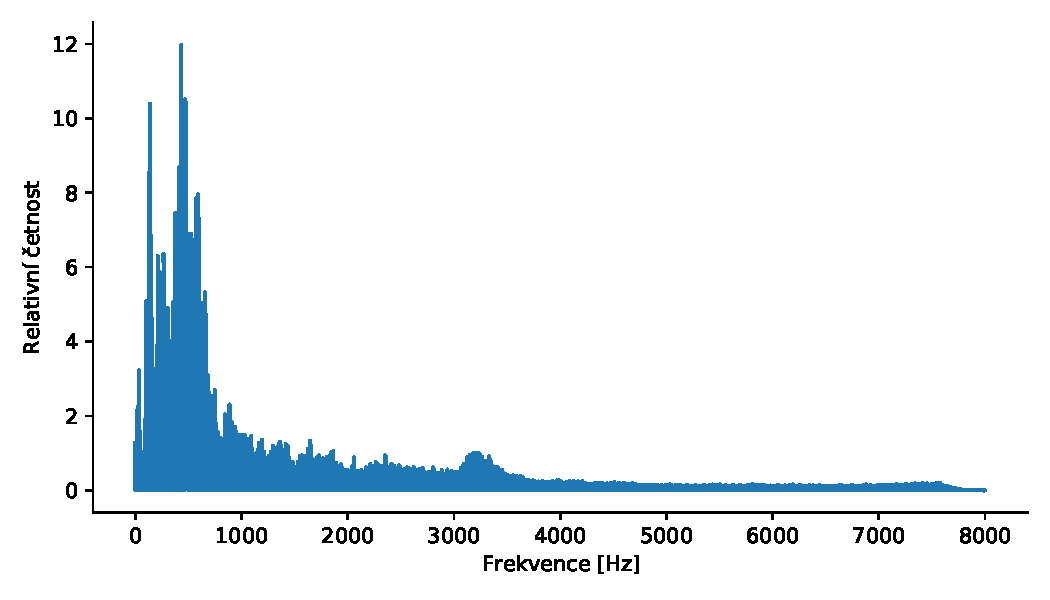
\includegraphics[width=\linewidth]{obrazky-figures/signal_spectrum.pdf}
  \caption{Spektrum signálu bez použití preemfáze.}
  \label{fig:Signal_without_preemphasis}
\end{figure}

\begin{figure}[ht!]
  \centering
  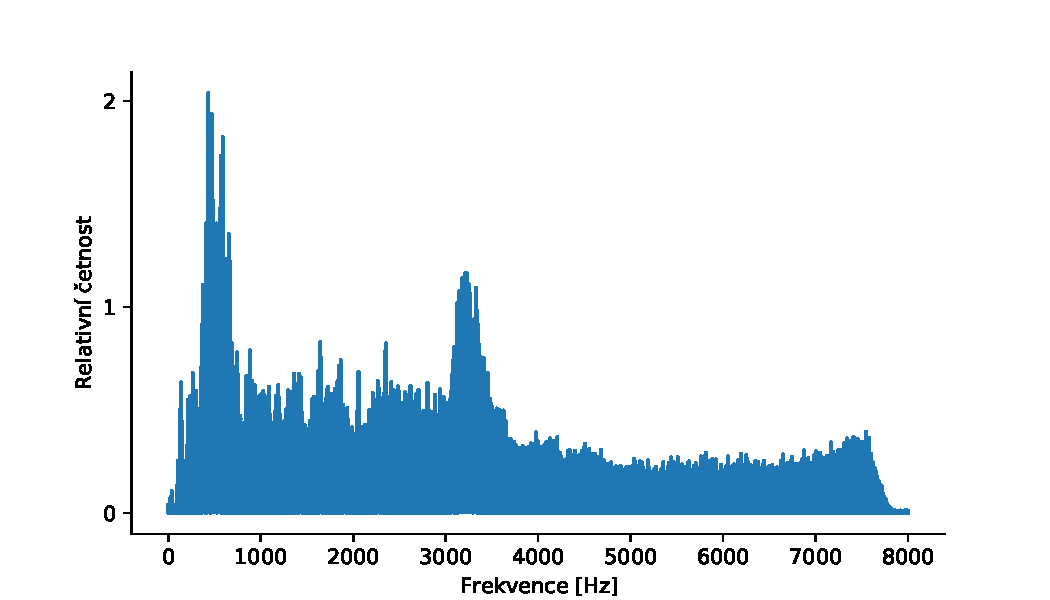
\includegraphics[width=\linewidth]{obrazky-figures/signal_spectrum_pre.pdf}
  \caption{Spektrum signálu po aplikaci preemfáze.}
  \label{fig:Signal_with_preemphasis}
\end{figure}

\subsection{Segmentace}
\label{subsection:Segmentation}
Řečový signál v~průběhu času mění svůj charakter vzhledem ke své povaze. Přístup, v~němž by extrakce příznaků audio nahrávky probíhala nad každým bitem signálů, je ale zcela nepředstavitelný. Řečový signál je však kvazistacionární, a tudíž je možné předpokládat, že $N$ sousedních vzorků reprezentuje stejnou informaci. Je nutné nalézt takové $N$, které je dostatečně malé na to, abychom hledané vlastnosti signálu mohli bezchybně vyjádřit $N$ vzorky a zároveň dostatečné velké, aby hledané vlastnosti nebyly ovlivněny lokálními změnami. Tyto protichůdné požadavky jsou vcelku splněny pro $N$ vzorků, které reprezentují úsek o~délce cca 10 až 25~ms. Zmíněné hodnoty odpovídají periodě změny hlasového ústrojí v~lidském těle. Za účelem odstranění ostrých hran je vhodné sousední segmenty překrývat. Překrývání úseků je výpočetně náročnější, ale je dosaženo částečného vyhlazení časových průběhů získaných parametrů. V~případě vyššího překrytí rámců je možné sledovat mezi sousedními rámci určitou závislost, která může způsobit selhání jistých klasifikačních technik předpokládajících nezávislost sousedních parametrů. Optimální hodnota překrytí segmentů se pohybuje okolo 50~\%~\cite{Sigmund_Analyza}. Princip segmentace je zobrazen na~\imageref{fig:Segmentation}{}.

\begin{figure}[ht]
  \centering
  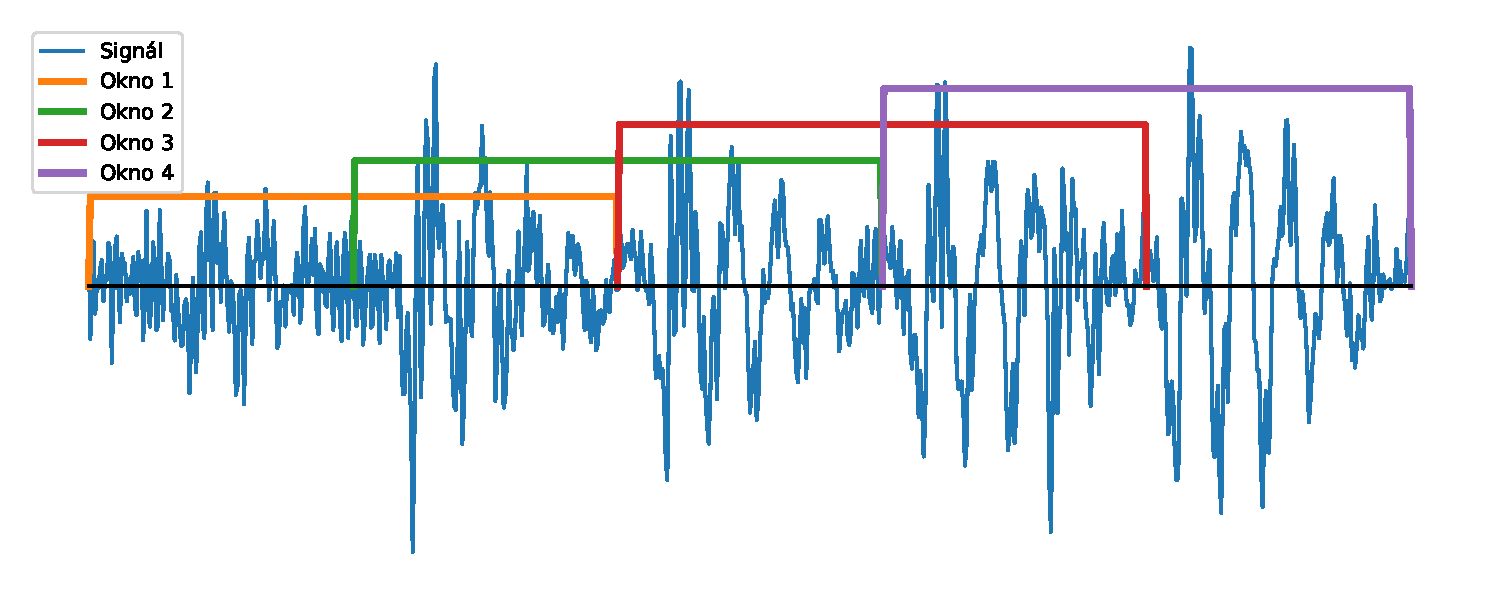
\includegraphics[width=\linewidth]{obrazky-figures/segmentation.pdf}
  \caption{Princip segmentace je znázorněný na signálu o~délce 50~ms. Signál je rozdělen na 4~segmenty o~velikosti 20~ms s~překrytím 10~ms.}
  \label{fig:Segmentation}
\end{figure}

Segmentace je dána vztahem
\begin{equation}
\label{eqn:Segmentation}
    \mathbf{y} = \mathbf{x} \times \mathbf{w},
\end{equation}
kde $\mathbf{x} \in \mathbb{R}^{N}$ je původní signál a $\mathbf{w} \in \mathbb{R}^{N}$ je vektor tzv. okénkové funkce, která je nulová mimo zvolený interval, symetrická kolem středu, maxima dosahuje většinou okolo středu intervalu a bývá klesající směrem od středu. V~obou případech a v~následujících vzorcích je $N$ rovné počtu vzorků signálu. Pomocí segmentace je možné z~nahrávky extrahovat příslušné vzorky a přidělit jim určitou váhu. Prakticky dochází nejdříve k~izolaci příslušného segmentu a následně k~násobení vzorků s~příslušnými váhami. Existuje mnoho variant tzv. okénkových funkcí, patří mezi ně např. pravoúhlé okno, trojúhelníkové okno, kosinové okno, Gaussovo okno, Hannovo okno, Blackmanovo okno a Kaiserovo okno, Hammingovo nebo Parzenovo okno. Nejčastěji používanými typy oken při zpracování řeči jsou
\begin{itemize}
    \item pravoúhlé okno
    \begin{equation}
    \label{eqn:Rectangular_window}
        f_{n} = \begin{cases}
                   1               & n \in \{M + 1, \dots, M + K\}\\
                   0               & \text{jinak}\\
               \end{cases}, n \in \{ 1, \dots, N\}
    \end{equation}
    
    \item Hammingovo okno
    \begin{equation}
    \label{eqn:Hamming_window}
        f_{n} = \begin{cases}
                   0,54 - 0,46\cos (\frac{2\pi \cdot (n - M)}{K})             & n \in \{M + 1, \dots, M + K\}\\
                   0               & \text{jinak}\\
               \end{cases}, n \in \{ 1, \dots, N\}.
    \end{equation}
   
\end{itemize}
V~obou případech $M$ označuje první segment, ve kterém je okno nenulové a $K$ délku okna. 
\begin{figure}[ht]
  \centering
  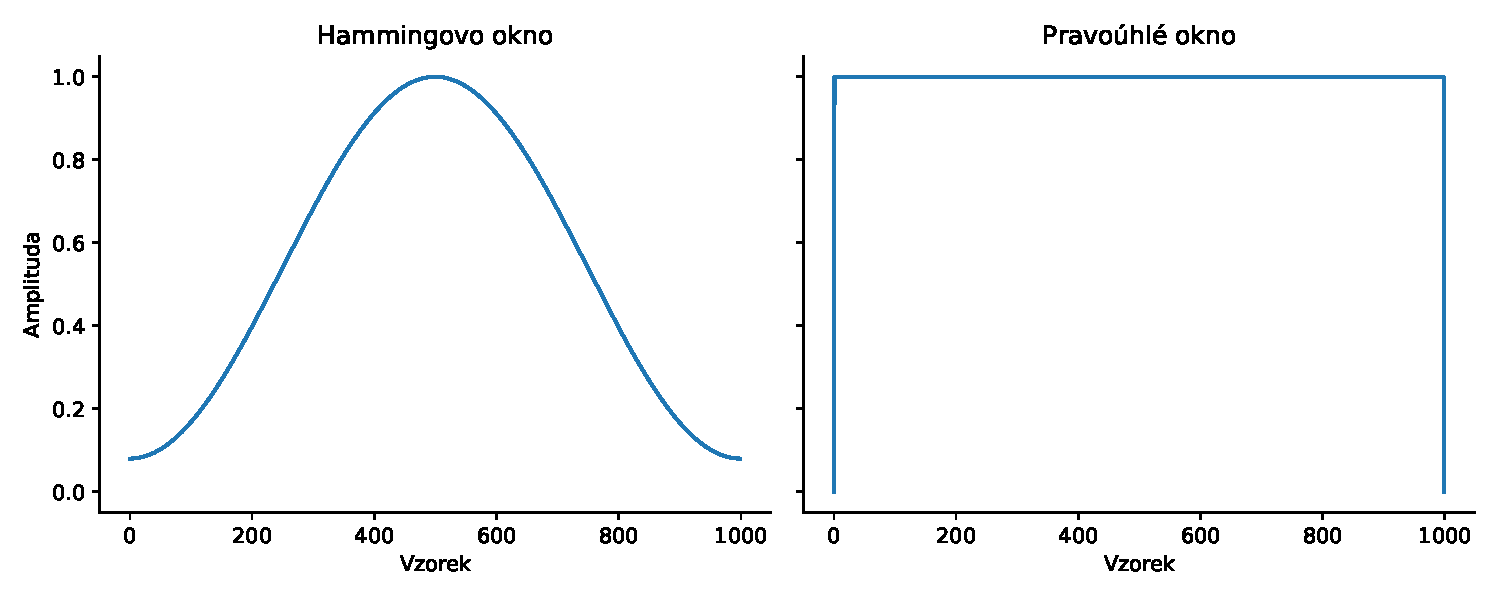
\includegraphics[width=\linewidth]{obrazky-figures/hamming_rectangular.pdf}
  \caption{Tvar Hammingova a pravoúhlého okna o~délkách 1000~vzorků.}
  \label{fig:windows}
\end{figure}

Okna jsou zobrazena na~\imageref{fig:windows}{}. V~obou případech je N rovno délce okna. Přestože se pravoúhlé okno jeví jako velmi jednoduché a výpočetně zcela nenáročné, většinou je používáno okno Hammingovo, a to z~důvodu vyšší stability výpočtů a nežádoucího rozmazání a rozptylu spektra, k~němuž dochází při použití okna pravoúhlého, což je zapříčiněno frekvenční charakteristikou pravoúhlého okna. Spektrum obsahuje jeden hlavní lalok a velké množství laloků vedlejších. Konvolucí spektra okna se spektrem signálu se jedna frekvence vstupního signálu zpropaguje mezi sousední frekvence. Použitím okna Hammingova dojde k~výraznějšímu \uv{rozmáznutí} spektra způsobeného dvojnásobnou šířkou hlavního laloku, které vede k~nižší frekvenční selektivitě. Z~praktických důvodů a kvůli vyšší stabilitě výpočtů je častěji používáno okno Hammingovo. Na~\imageref{fig:Hamming_rectangular_spektrum}{0} jsou zobrazeny frekvenční odezvy pravoúhlého a Hammingova okna.

\begin{figure}[ht]
  \centering
  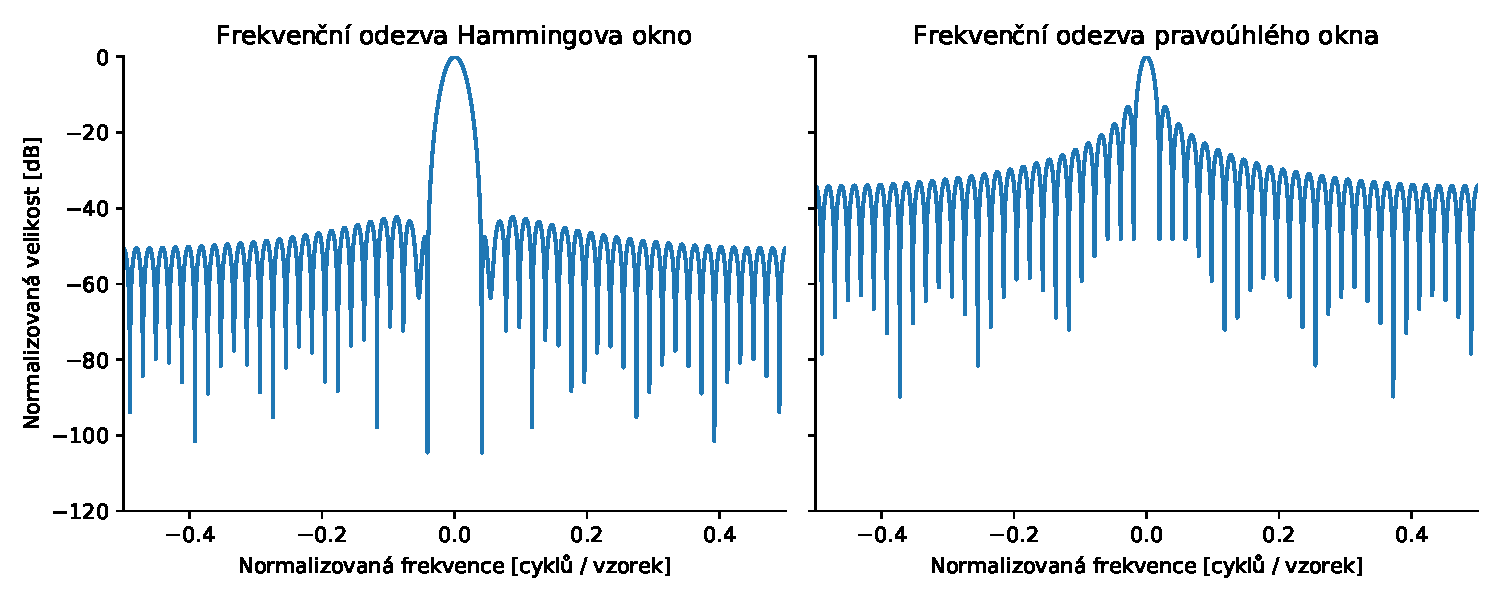
\includegraphics[width=\linewidth]{obrazky-figures/hamming_rectangular_spektrum.pdf}
  \caption{Frekvenční odezva pravoúhlého a Hammingova okna. Lze pozorovat zmiňovanou šířku hlavního laloku a rozdíl mezi energií hlavního a vedlejších laloků. Z~výše uvedených důvodu je vhodnější použít okno Hammingovo.}
  \label{fig:Hamming_rectangular_spektrum}
\end{figure}

Řečový signál je aplikováním $W$ oken o~délce $K$ a následnou filtrací nulových hodnot rozdělen do $W$ segmentů o~konstantní délce segmentu $K$ vzorků. Energetické spektrum segmentů je vyrovnanější a částečně je odstraněn šum. Takto získané segmenty můžeme dále analyzovat a aproximovat konstantními parametry.  


%%%%%%%%%%%%%%%%%%%%%%%%%%%%%%


\section{Parametry řečového signálu}
Jak již bylo zmíněno v~podsekci~\ref{subsection:Segmentation}, řeč je kvazistacionární a její segmenty můžeme považovat za stacionární, jelikož ke změnám dochází dostatečně pomalu. Tento předpoklad nám umožňuje segmenty reprezentovat konstantními parametry a není nutné provádět jejich  výpočet nad každým bitem digitalizovaného signálu. Příslušné vzorky segmentů signálu obsahují vysoké množství informací. Některé z~nich jsou pro účely této práce irelevantní. Cílem této sekce je představit nejdůležitější parametry aproximující úsek řeči pro potřeby psychoterapie a popsat způsob jejich extrakce. 
% https://www.ncbi.nlm.nih.gov/pmc/articles/PMC7042657/

\subsection{Energie signálu}
\label{subsection:Energy}
Střední krátkodobá energie signálu se v~časové doméně definuje jako velikost skalárního součinu signálu se sebou samým. U~diskrétního signálu $\mathbf{s}$ o~délce segmentu $N$ je dána vztahem

\begin{equation}
\label{eqn:Energy}
    E = \sum_{n=1}^{N} {\lvert s_{n} \rvert}^2.
\end{equation}

U~řečových signálů neobsahujících šum a zvuky okolí může energie signálu sloužit k~jednoduché detekci řečové aktivity. Energie signálu je u~znělých hlásek podstatně vyšší než u~neznělých. Podle tohoto kritéria lze fonémy rozdělit do pěti skupin: samohlásky, nosovky, znělé frikativy, neznělé frikativy a mezery v~řeči~\cite{Sigmund_Analyza}.

\subsubsection{Střední kvadratická energie}
\label{subsection:RMSE}
Dalším způsobem výpočtu energie signálu je jeho střední kvadratická energie (RMSE -- root mean square energy). Vede k~zvýraznění úseků, při nichž dochází k~řečové aktivitě~\cite{Simak_adaptive_energy_VAD}. Je dána vztahem
\begin{equation}
\label{eqn:RMSE}
    RMSE = \sqrt{\frac{1}{N} \sum_{n=1}^{N} {\lvert s_{n} \rvert}^2}.
\end{equation}

\imageref{fig:Energy}{1} znázorňuje rozdíl mezi energií a střední kvadratickou energií. 

\begin{figure}[ht]
  \centering
  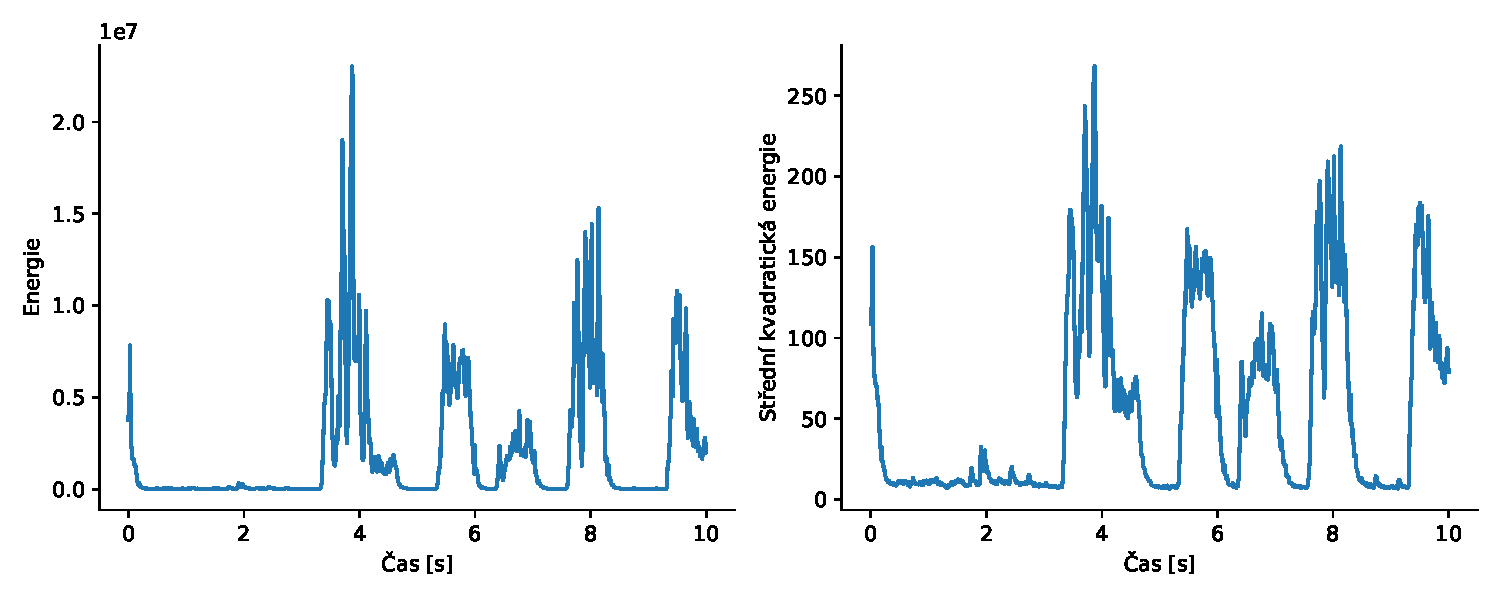
\includegraphics[width=\linewidth]{obrazky-figures/energy.pdf}
  \caption{Energie a střední kvadratická energie segmentů signálu. U~střední kvadratické energie lze pozorovat vyšší energii řečově aktivních segmentů v~poměru s~tichem.}
  \label{fig:Energy}
\end{figure}

\subsubsection{Normalizovaná energie}
Abychom odstranili varianci mezi příslušnými nahrávkami, kanály a řečníky, je vhodné energii normalizovat do rozsahu $\langle-1,1\rangle$. Toho lze docílit následujícím vztahem
\begin{equation}
\label{eqn:Energy_norm}
    Enorm_{n} = \frac{E_{n} - \mu}{\lambda},
\end{equation}
kde $\mathbf{E}$ je vektor středních krátkodobých energií segmentů, $\mu$ jejich střední hodnota a $\lambda$ jejich směrodatná odchylka.


\subsection{Mel-frekvenční cepstrální koeficienty}
\label{subsection:MFCC}
Jak již bylo zmíněno v~sekci~\ref{section:Speech_signal}, zvuk je buzení vznikající v~hlasivkové štěrbině, které je následně filtrováno tvarem hlasového traktu jedince. Tento tvar určuje, jaký zvuk vychází. Pokud lze přesně určit tento tvar, pak je i možné poskytnout přesnou reprezentaci vytvářeného fonému. Cílem je oddělit buzení a získat tvar traktu. Ten se projevuje v~krátkodobém výkonovém spektru. Úkolem Mel-frekvenčních cepstrálních koeficientů (MFCC -- Mel-frequency cepstral coefficients) je co nejpřesněji reprezentovat tvar hlasového traktu řečníka. MFCC představili v~80. letech 20. století Steven B. Davis a Paul Mermelstein~\cite{Davis_Mermelstein_MFCC} a od té doby patří mezi nejpoužívanější příznaky využívané k~rozpoznání řeči a řečníka.

\subsubsection{Melova stupnice}
MFCC díky nelineární transformaci do Melovy stupnice na rozdíl od DFT-cepstra aproximují lépe lidský sluch, který je výrazně citlivější na rozdíly v~nižších frekvencích. Převodem do Melovy stupnice je pro lidské ucho rozdíl mezi 0 a 100~Mely stejný jako mezi 100 a 200~Mely, což neplatí pro frekvenci~\cite{huang_acero_hon_2005}. Převod z~frekvence $f$ do Melovy stupnice $m$ je dán vztahem

\begin{equation}
\label{eqn:Freq_to_mel}
    M(f) = 1125 \ln(1 + \frac{f}{700})
\end{equation}

\noindent a podobně z~Melovy stupnice na frekvenci

\begin{equation}
\label{eqn:Mel_to_freq}
    M^{-1}(m) = 700(e^{\frac{m}{1125}}-1).
\end{equation}

\subsubsection{Melova banka filtrů}
Výkonové spektrum signálu informuje o~tom, jak silně je která frekvence v~signálu zastoupená. Obsahuje však také mnoho informací, které jsou pro rozpoznání zbytečné. Lidské ucho téměř nedokáže rozlišit velmi blízké frekvence a zároveň, jak je popsáno výše, vnímá jinak rozdíl mezi frekvencemi určitého řádu. Vytvořením banky filtrů a jejím součinem s~výkonovým spektrem jsou získány rovnoměrně rozložené koeficienty reprezentující zastoupení příslušných intervalů frekvencí v~řeči~\cite{lyons_mfcc}.

Prvním krokem tvorby banky filtrů je určení spodní a horní hranice frekvencí, pro něž je banka tvořena. Tyto frekvence jsou převedeny do Melovy stupnice pomocí rovnice~\ref{eqn:Freq_to_mel} a je nutné vytvořit N\footnote{počet MFCC koeficientů} rovnoměrně rozložených intervalů. Hranice intervalů jsou následně převedeny zpátky do Hertzů podle vztahu~\ref{eqn:Mel_to_freq}. Tím získáváme hranice intervalů v~Hertzích a zbývá pouze převést tato čísla do indexů vektoru výkonového spektra~\cite{lyons_mfcc}.

Nad získanými indexy vytvoříme N trojúhelníkových oken znázorněných na~\imageref{fig:Mel_filter_bank}{0} podle následujícího vztahu

\begin{equation}
    \label{eqn:Mel_filter}
    H_m[k] = \begin{cases}
                0                                 & k < f[m -1]\\
                \frac{k - f[m - 1]}{f[m] - f[m - 1]}    & f[m - 1] <= k <= f[m]\\
                \frac{f[m + 1] - k}{f[m + 1] - f[m]}    & f[m] <= k <= f[m + 1]\\
                0                                 & k > f[m + 1]\\
               \end{cases},
\end{equation}
kde \textbf{f} je vektor indexů hranic bank, \textbf{m} příslušné okno a \textbf{k} index pole o~velikosti rozlišení výkonového spektra.

\begin{figure}[ht]
  \centering
  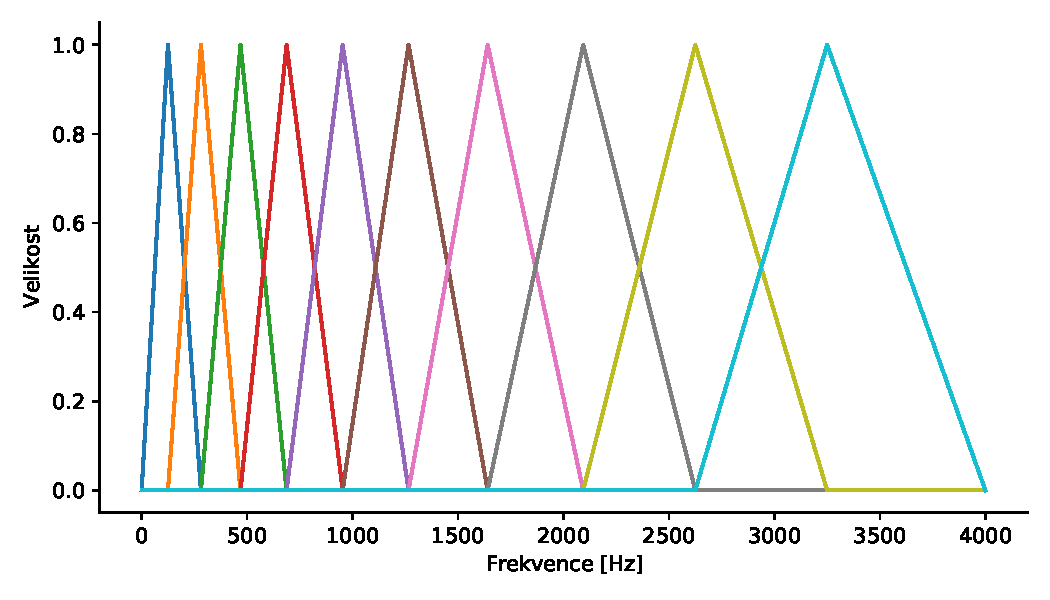
\includegraphics[width=\linewidth]{obrazky-figures/mel_bank.pdf}
  \caption{Melova banka filtrů pro signál s~vzorkovací frekvencí 8~kHz, s~rozlišením výkonového spektra 512~vzorků pro 10~MFCC koeficientů.}
  \label{fig:Mel_filter_bank}
\end{figure}


\subsubsection{Získání MFCC}
Mel-frekvenční cepstrální koeficienty jsou získány následujícím způsobem:
\begin{itemize}
    \item signál je rozdělen do krátkých segmentů při použití okénkové funkce -- nejčastěji je použito Hammingovo okno
    \item na segmenty je aplikována diskrétní Fourierova transformace 
    \item pro každý segment je vypočteno jeho výkonové spektrum -- normalizací mocniny absolutní hodnoty výstupu diskrétní Fourierové transformace
    \item je provedena nelineární transformace energií příslušných frekvencí do Melovy stupnice a je sečtena suma energií příslušných filtrů 
    \item nad logaritmem energií banky filtrů je provedena diskrétní kosinová transformace
\end{itemize}
\imageref{fig:MFCC_process}{1} zobrazuje proces extrakce MFCC příznaků jednoho segmentu o~délce 20~ms signálu.

\begin{figure}[ht]
  \centering
  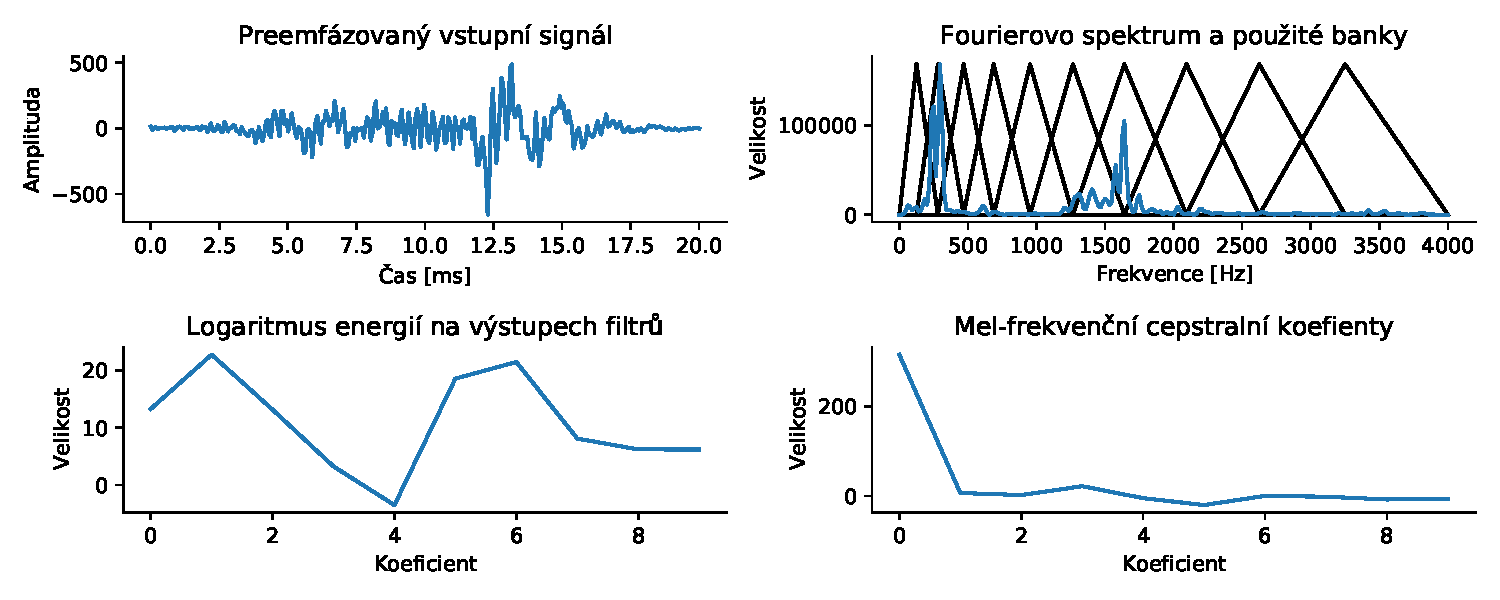
\includegraphics[width=\linewidth, height=\textheight / 3]{obrazky-figures/mfcc.pdf}
  \caption{Extrakce 10~MFCC příznaků ze segmentu o~délce 20~ms signálu vzorkovaného 8000~{vzorků}/{s} s~rozlišením 512~vzorků frekvenčního spektra. Nad vstupním signálem je provedena preemfáze a následná segmentace s~využitím Hammingova okna. Jeden z~takto získaných segmentů je zobrazen nahoře vlevo. Nad signálem obsaženým v~segmentu je provedena diskrétní Fourierova transformace a je vypočteno výkonové spektrum. Obrázek vpravo nahoře ukazuje výkonové spektrum a použitou banku filtrů. Následně na obrázku vlevo dole je zobrazen logaritmus sumy energií příslušných filtrů. Nad energií filtrů je provedena diskrétní kosinová transformace, která je zobrazena na obrázku vpravo dole.}
  \label{fig:MFCC_process}
\end{figure}

\subsubsection{Delta koeficienty}
Získané MFCC koeficienty lze ještě rozšířit o~delta, případně delta-delta MFCC, které obsahují informace o~změnách příznaků mezi sousedními segmenty, definované jako

\begin{equation}
    \label{eqn:MFCC_delta}
    D[k][m] = \frac{\sum_{n=1}^{N} n(C[k+n][m] - C[k-n][m])}{2 \sum_{n=1}^{N} n^2}, k \in \{1,\dots,K\},  m \in \{1,\dots,M\},
\end{equation}

kde $K$ je počet segmentů signálu, $M$ počet MFCC koeficientů, N počet sousedních segmentů, nad kterými má být výpočet dynamiky proveden a \textbf{C} je matice MFCC koeficientů o~velikosti $K \times M$. Delta příznaky jsou podle vztahu~\ref{eqn:MFCC_delta} vypočítány nad MFCC příznaky, a obdobně delta-delta nad delta koeficienty~\cite{lyons_mfcc}.

%%%%%%%%%%%%%%%%%%%%%%%%%%%%%%

\section{Shlukovací algoritmy}
Shlukovací algoritmy slouží k~třídění dat do skupin (shluků) tak, aby si data náležející do stejné skupiny byla co nejvíce podobná a zároveň variance mezi třídami byla co nejvyšší. Cílem shlukové analýzy je se co nejjednoznačněji rozhodnout, do které skupiny \uv{dato} náleží. V~této práci jsou shlukovací algoritmy použity v~procesu detekce řečové aktivity a diarizace.

\subsection{Směs Gaussovských rozložení}
\label{subsection:GMM}
Směs Gaussovských rozložení (GMM -- Gaussian Mixture Model) je parametrická funkce hustoty pravděpodobnosti reprezentovaná jako vážený součet hustot Gaussovských komponent. Sekce vychází z~následujícího článku~\cite{Reynolds2009GaussianMM}.

GMM se běžně používají jako parametrický model distribuce pravděpodobnosti kontinuálních měření nebo v~biometrických systémech. Parametry modelu (váhy, střední hodnoty a kovariační matice) jsou odhadnuty z~trénovacích dat pomocí iteračního algoritmu Expectation-Maximization (EM), jelikož neexistuje žádné analytické řešení pro odhad těchto parametrů. V~některých případech může být využit i Viterbiho algoritmus, který je velmi intuitivní, avšak kvůli vysoké pravděpodobnosti uvíznutí v~lokálním minimu nemusí vždy vést k~nalezení globálního optima.

Gaussovská směsice je reprezentována jejími středními hodnotami, kovariančními maticemi a váhami příslušných komponent. Tyto parametry jsou společně reprezentovány následující anotací

\begin{equation}
    \label{eqn:GMM_params}
    \mathbf{\Lambda} = \{\omega_i, \text{\boldmath$\mu$}_{i}, \mathbf{\Sigma_i}\}\quad \text{pro}\quad, i \in \{1, \dots, M\},
\end{equation}

kde $M$ je počet komponent Gaussovské směsice, $\text{\boldmath$\mu$}_{i}$ vektor středních hodnot a $\mathbf{\Sigma}_i$ kovarianční matice. Váhy komponent $\omega_{i}$ splňují následující rovnici

\begin{equation}
    \label{eqn:GMM_weights_sum}
    \sum_{i=1}^{M} \omega_i = 1.
\end{equation}

Kovarianční matice $\mathbf{\Sigma}_{i}$ modelu $\mathbf{\Lambda}$ mohou být omezeny na diagonální matici, v~takovém modelu předpokládáme, že vzorky modelované veličiny jsou na sobě statisticky nezávislé. Kovarianční matice mohou být taktéž sdílené mezi komponentami. Směs Gaussovských rozložení je vážená suma M komponent Gaussovských hustot daná vztahem

\begin{equation}
    \label{eqn:GMM}
    p(\mathbf{x}|\Lambda) = \sum_{i=1}^{M} \omega_i \cdot \mathcal{N}(\mathbf{x}|\text{\boldmath$\mu$}_{i},\mathbf{\Sigma}_{i}),
\end{equation}

kde $\mathbf{x}$ je D-dimenzionální vektor (reprezentující objekt ze skupiny sledovaných dat), $\omega_i$ váha příslušné komponenty, a $\mathcal{N}(\mathbf{x}|\text{\boldmath$\mu$}_{i},\mathbf{\Sigma}_{i})$ hustota Gaussovské komponenty. Příslušné hustoty komponent Gaussovské směsice odpovídají hustotám D-rozměrných normálních rozložení definovaných jako

\begin{equation}
    \label{eqn:Normal_distribution}
    \mathcal{N}(\mathbf{x}|\text{\boldmath$\mu$}_{i},\mathbf{\Sigma}_{i}) = \frac{1}{(2\pi)^{D/2}|\mathbf{\Sigma}_i|^{1/2}} e^{-\frac{1}{2}(\mathbf{x} - \text{\boldmath$\mu$}_{i})^T \mathbf{\Sigma}^{-1} (x - \text{\boldmath$\mu$}_{i})},
\end{equation}

Jak již bylo zmíněno, směs Gaussovských rozložení je velmi často využívána v~biometrických systémech, resp. systémech rozpoznání mluvčího, kde dokáže velmi dobře reprezentovat velkou třídu dat příslušné distribuce.  
\subsubsection{EM algoritmus}
Již bylo vysvětleno, jaké parametry reprezentují GMM, ale otázkou zůstává, jak nalézt takové parametry, aby věrohodnost trénovacích dat byla jak nejvyšší. Existuje mnoho technik pro nalezení optimálních parametrů, nejznámější a nejvíce používanou je Expectation Maximization algoritmus. Expectation Maximization~\cite{Dempster77maximumlikelihood} je iterativní algoritmus pro trénování generativních modelů se skrytými proměnnými. Každá iterace tohoto algoritmu vede ke zvýšení věrohodnosti trénovacích
dat. Algoritmus ovšem nezaručuje nalezení globálního optima.

Pro posloupnost T tréninkových dat $\mathbf{X} = \{\mathbf{x}_{1}, \cdot, \mathbf{x}_{T}\}$, věrohodnost GMM, za předpokladu nezávislosti mezi trénovacími daty, můžeme zapsat jako
\begin{equation}
    \label{eqn:GMM_likelihood}
    p(\mathbf{X}|\mathbf{\Lambda}) = \prod_{t=1}^{T} p(\mathbf{x_t}|\mathbf{\Lambda}).
\end{equation}

Tento výraz je bohužel nelineární funkcí parametrů $\mathbf{\Lambda}$ a přímá maximalizace není možná. Naštěstí je možné nalézt maximálně věrohodné (ML -- Maximum Likelihood) parametry iterativně. Základní myšlenkou je, vycházeje z~modelu reprezentovaným parametry $\mathbf{\Lambda}_{old}$, odhadnout nové parametry $\mathbf{\Lambda}_{new}$ tak, že $p(\mathbf{X}|\mathbf{\Lambda}_{new}) >= p(\mathbf{X}|\mathbf{\Lambda}_{old})$. Nový model bude dále inicializačním modelem dalšího kroku a iterační algoritmus pokračuje, dokud není splněna ukončující podmínka, kdy rozdíl věrohodnosti nového a starého modelu je menší než práh $F$.
\begin{equation}
    \label{eqn:GMM_thresh}
   p(\mathbf{X}|\mathbf{\Lambda}_{new}) - p(\mathbf{X}|\mathbf{\Lambda}_{old}) < F
\end{equation}

V~každé iteraci dochází k~výpočtu nových parametrů modelu. Nejdříve jsou v~kroku E~(Expectation step) vypočteny statistiky, konkrétně věrohodnosti příslušných komponent Gaussovské směsice vůči datům. V~kroku M~(Maximalization step) dochází k~aktualizaci parametrů $\mathbf{\Lambda}$ podle následujících vztahů tak, aby věrohodnost modelu vůči trénovacím datům byla opět co nejvyšší.
\begin{enumerate}
    \item Krok E: \begin{itemize}
                        \item Věrohodnost $\gamma_{ct}$ Gaussovské komponenty $c$ vůči vektoru dat $\mathbf{x}_{t}$ a parametrům $\mathbf{\Lambda}_{old}$
                            \begin{equation}
                                \label{eqn:GMM_components}
                                P(c|\mathbf{x}_t, \mathbf{\Lambda}_{old}) = \frac{\omega_c^{old} \mathcal{N}(\mathbf{x}_{t}|\text{\boldmath$\mu$}_{c}^{old},\mathbf{\Sigma}_{c}^{old})}{\sum_{k=1}^{M}\omega_k^{old} \mathcal{N}(\mathbf{x_t}|\text{\boldmath$\mu$}_{k}^{old},\mathbf{\Sigma}_{k}^{old})} = \gamma_{ct}
                            \end{equation}
                    \end{itemize}
    \item Krok M:   \begin{itemize}
                        \item Nové váhy modelu
                            \begin{equation}
                                \label{eqn:GMM_weights}
                                \omega_c = \frac{1}{T} \sum_{t=1}^T \gamma_{ct}, c \in \{1, \dots, M\}
                            \end{equation}
                        \item Nové střední hodnoty
                            \begin{equation}
                                \label{eqn:GMM_means}
                                \text{\boldmath$\mu$}_c = \frac{\sum_{t=1}^{T} \gamma_{ct} \mathbf{x}_{t}}{\sum_{t=1}^T \gamma_{ct}},c \in \{1, \dots, M\}
                            \end{equation}
                        \item Nové rozptyly (kovarianční matice)
                            \begin{equation}
                                \label{eqn:GMM_cov}
                                \mathbf{\Sigma}_c^{2} = \frac{\sum_{t=1}^{T} \gamma_{ct} \mathbf{x}_t^{2}}{\sum_{t=1}^T \gamma_{ct}} - \text{\boldmath$\mu$}_c^{-2}, c \in \{1, \dots, M\}
                            \end{equation}
                    \end{itemize}
\end{enumerate}

%%%%%%%%%%%%%%%%%%%%%%%%%%%%%%

\section{Detekce řečové aktivity}
\label{section:VAD}
Segmentovaný signál nahrávky lidské řeči obsahuje vysoký podíl segmentů, kde se vyskytuje pouze šum okolí, případně nedochází k~žádné řečové aktivitě mluvčího. Detekce řečové aktivity (VAD -- Voice activity detecion) je úloha zabývající se určením, kdy opravdu dochází k~mluvě. Tato úloha je základním kamenem všech systémů zabývajících se kódováním řeči, rozlišením řečníků v~nahrávce, extrakci informací o~mluvčích z~nahrávky nebo systémů monitorujících zákaznická call centra. VAD je obvykle prvním stavebním kamenem těchto systémů. Cílem je co nejpřesněji a za co nejnižší výpočetní náklady rozlišit segmenty řečové aktivity od těch, které obsahují ticho, šum. Existuje mnoho řešení, začínajících od základních algoritmů, rozhodujících se pouze podle střední krátkodobé energie signálu, až po algoritmy používající spojení vícero komplexních modelů. \imageref{fig:VAD}{1} znázorňuje, jak by měl takový systém fungovat.   


\begin{figure}[ht]
  \centering
  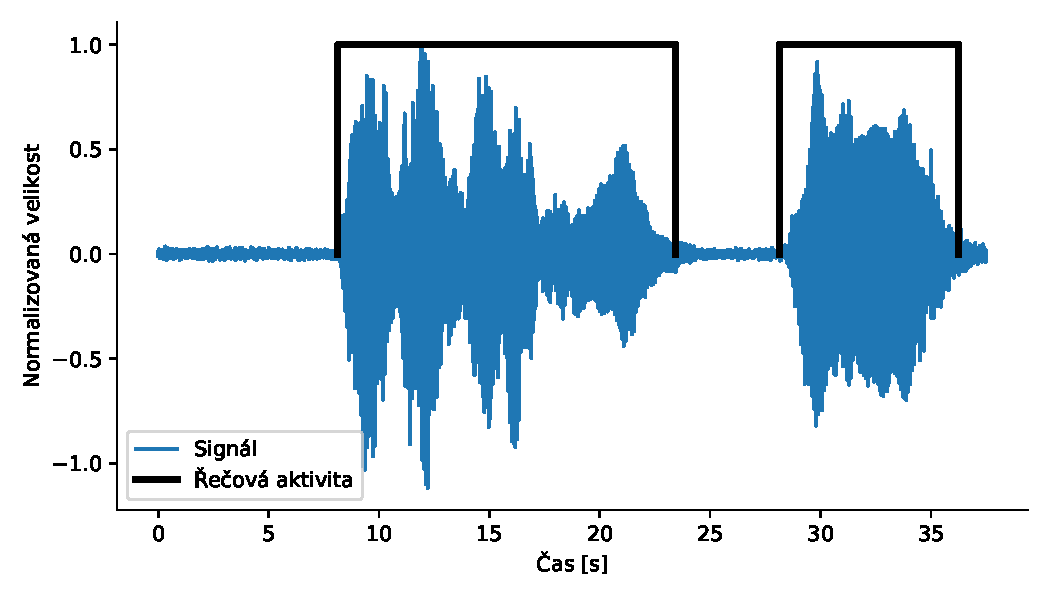
\includegraphics[width=\linewidth]{obrazky-figures/signal_vad.pdf}
  \caption{Detekce řečové aktivity na signálu o~délce 8~sekund. Úseky, ve kterých je okno v~hodnotě 1, jsou považovány za úseky řečové aktivity řečníka. Úseky okna v~0 reprezentují ticho.}
  \label{fig:VAD}
\end{figure}

Obvyklé algoritmy detekce řečové aktivity nejdříve extrahují příznaky daného úseku nahrávky a ty se následně klasifikují pomocí diskriminačních modelů. Většina VAD systémů provádí tvrdé rozhodnutí na řeč a ticho. \imageref{fig:VAD_graph}{1} znázorňuje koncepci základního detektoru řečové aktivity~\cite{VAD_overview}. 

\begin{figure}[ht]
  \centering
  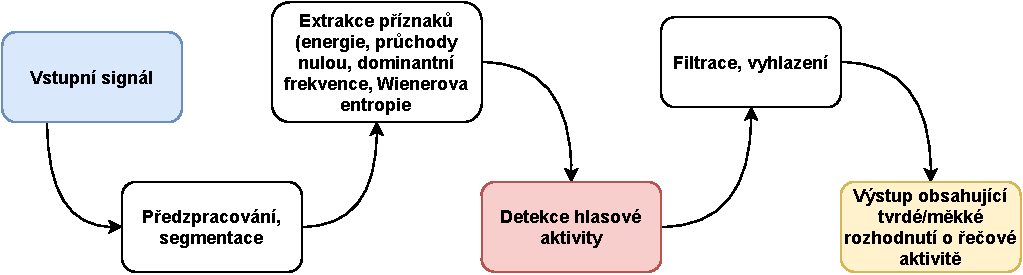
\includegraphics[width=\linewidth]{obrazky-figures/vad_diagram.pdf}
  \caption{Blokový diagram systému detekce řečové aktivity. Vstupní signál je předzpracován a segmentován do N úseků stejné délky. Ze segmentů jsou extrahovány příznaky, pomocí kterých je rozhodnuto, zda se jedná o~řečově aktivní úsek. Výstup je následně vyhlazen a jsou odstraněny špičky.}
  \label{fig:VAD_graph}
\end{figure}


Některé systémy provádějí rozhodnutí nad rámci, které mohou reprezentovat úseky řeči o~délce zhruba 10~ms, avšak délky fonému slovanských jazyků se pohybují někde mezi jednotkami až vyššími stovkami~ms~\cite{Pl_phonemes}. Z~toho vyplývá, že statisticky v~absolutní většině případů bude délka promluvy zahrnovat více než 1~segment. Taktéž nemusí být vždy úplně vhodné detekovat ticho o~délce 10~ms v~delším úseku plynulé řeči. Řešením je provést postprocessing a odstranit krátké úseky řeči/ticha. Existuje mnoho metod, kterými je možné vyhladit výstup systému VAD. Mezi běžně používané patří různé filtry jako třeba mediánový nebo průměrový filtr~\cite{gupta_filters}. Lze taktéž využít předpokladu, že data pocházejí ze skrytého Markovova modelu (HMM)~\cite{Cernocky_ZRE} a použít forward-backward algoritmus s~přechodovou maticí modelující pravděpodobnost přechodu ze stavu řeč/ticho a opačně~\cite{Bishop_pattern}. \imageref{fig:VAD_smooth}{1} demonstruje jeden ze způsobů vyhlazení řečové aktivity.

\begin{figure}[ht]
  \centering
  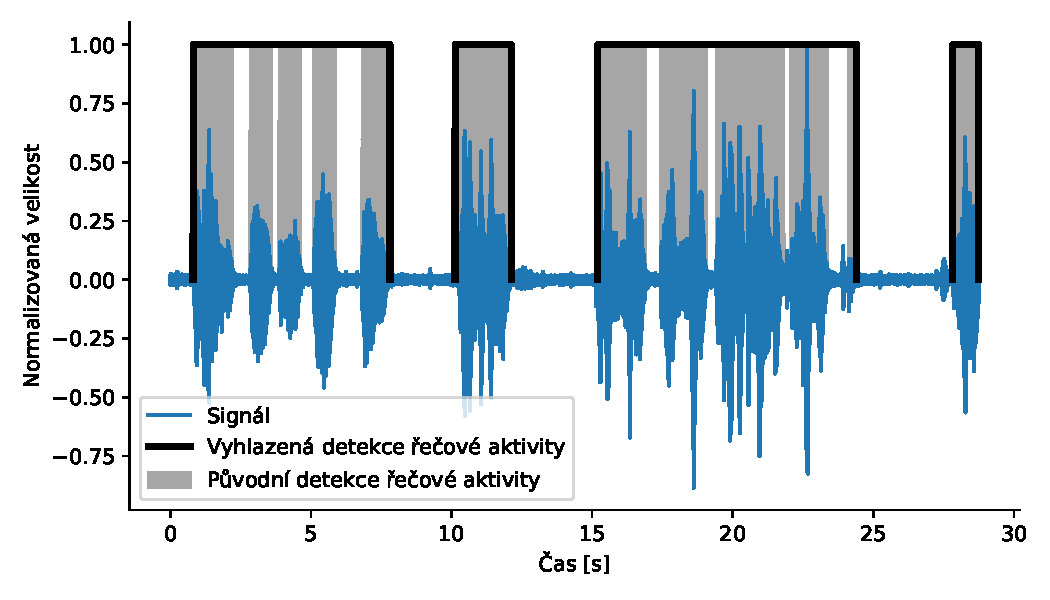
\includegraphics[width=\linewidth]{obrazky-figures/signal_vad_smooth.pdf}
  \caption{Detekce řečové aktivity. Nad segmenty, které byly označeny za řečově aktivní, je provedeno filtrování. Hodnoty řečové aktivity v~úsecích ticha, případně mluvy o~délce menší než 500 milisekund byly negovány, čímž vznikly plynulé úseky mluvy.}
  \label{fig:VAD_smooth}
\end{figure}

\subsection{Energetické VAD}
\label{subsection:Energy_VAD}
Detekovat řečovou aktivitu lze velmi dobře podle energie signálu v~případě, že signál není velmi výrazně \uv{zašumělý}. Energeticky vyšší segmenty lze považovat za řeč, segmenty se střední energií jako šum a nízko-energetické segmenty jako ticho. V~případě normalizované energie $E \in (-1,0;1,0)$ lze předpokládat, že ticho má zápornou energii, šum se pohybuje kolem 0 a řeč je reprezentována kladnou energií. Takto navržený systém však nedokáže rozpoznat energii mluvy a energii zvuku, který dokážou vyvolat jiné objekty kolem nás. Většina moderních mikrofonů však dokáže potlačit tyto okolní zvuky a lze předpokládat, že psychoterapeutická sezení probíhají v~tichých, klidných prostorech.

\subsubsection{Prahování}
\label{subsection:VAD_threshold}
Velmi jednoduchým, ale přesto celkem efektivním algoritmem je prahování podle energie segmentů. Prahovací funkce je definována jako  
\begin{equation}
    \label{eqn:E_threshold}
    f_{n} = \begin{cases}
                   1               & E_{n} >= T\\
                   0               & E_{n} < T\\
            \end{cases}, n \in \{1, \dots N\}
\end{equation}
kde $\mathbf{E}$ je vektor energií segmentů signálu, $T$ energetický práh a $N$ počet segmentů signálu.

Tento algoritmus může být rozšířen o~další příznaky, jako je počet průchodů nulou, dominantní frekvenci spektra nebo Wienerovu entropii~\cite{VAD_SFM}. Poté je nutné určit, zda je postačující, aby byla splněna jedna podmínka, nebo zda musí být splněny všechny, aby byl segment klasifikován jako řeč. Ačkoliv se jedná o~vcelku jednoduchý algoritmus, je nutné nastavit všechny prahy manuálně, což v~případě vysoké variance mezi nahrávkami může způsobovat špatné výsledky. Prahy lze dynamicky získat z~prvních $M$ segmentů ($\pm 50$ ms), u~kterých lze předpokládat ticho na začátku nahrávky. \imageref{fig:VAD_energy_threshold}{1} znázorňuje demonstrační příklad prahování signálu podle energie.

\begin{figure}[ht]
  \centering
  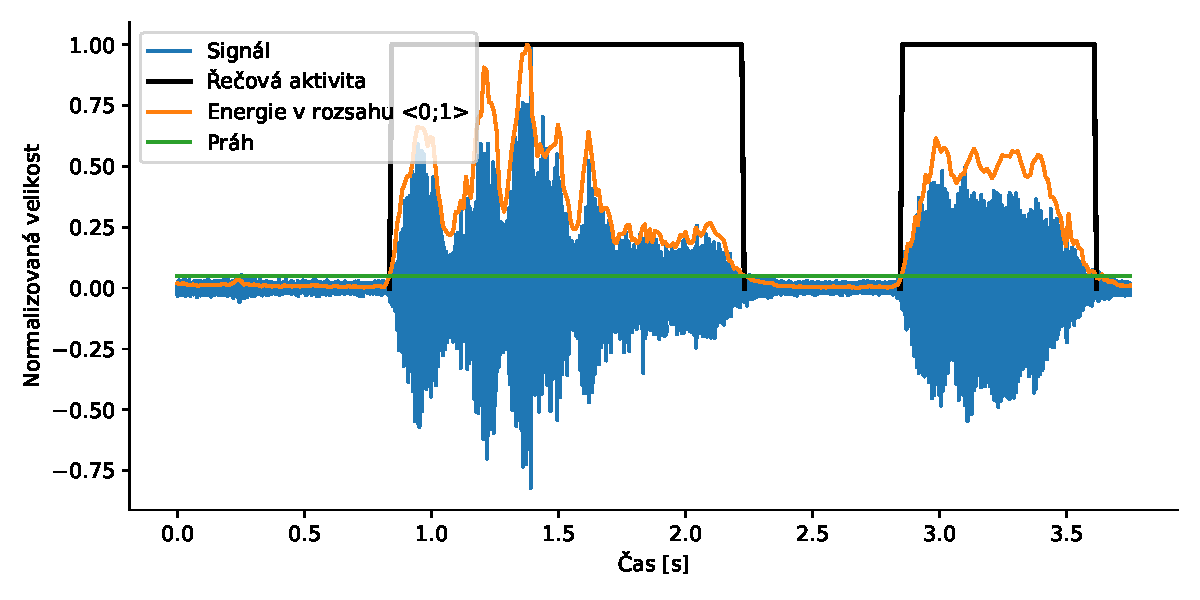
\includegraphics[width=\linewidth]{obrazky-figures/signal_vad_threshold.pdf}
  \caption{Detekce řečové aktivity pomocí prahování energie. Hodnota prahu je rovna $0,05$ v~relativním měřítku, segmenty s~relativní energií menší než práh jsou klasifikovány jako ticho a segmenty s~vyšší energií jako řeč.}
  \label{fig:VAD_energy_threshold}
\end{figure}

\subsubsection{Adaptivní práh}
\label{subsection:VAD_adaptive_threshold}
Jak bylo zmíněno v~předchozí podsekci~\ref{subsection:VAD_threshold} systémy založené na prahování nedokážou upravovat hodnotu prahu dynamicky a ne vždy je možné nastavit práh pro zcela odlišné nahrávky. Hlavní myšlenkou tohoto algoritmu je adaptivní aktualizace prahu pomocí výpočtu minimální a maximální hodnoty energií doposud zpracovaných segmentů. Tímto odpadá nutnost inicializace prahu před spuštěním~\cite{Simak_adaptive_energy_VAD}.

Algoritmus pracuje se střední kvadratickou energií popsanou v~podsekci~\ref{subsection:RMSE}. Algoritmus postupně prochází segmenty a aktualizuje maximální energii $\mathbf{X}$ a minimální energii $\mathbf{M}$. Všechny následující vzorce jsou definovány pro  $n \in \{1, \dots, N \}$, kde $N$ je počet segmentů signálu.

\begin{equation}
    \label{eqn:E_dynamic_threshold_max}
    X{n} = max(E_{n}, X_{n-1}),
\end{equation}

\begin{equation}
    \label{eqn:E_dynamic_threshold_min}
    M_{n} = min(E_{n}, j_{n-1} \cdot M_{n-1}),
\end{equation}


kde $max(a,b)$ je funkce vracející větší číslo z~dvojice $a,b$ a $min(a,b)$ funkce vracející menší číslo z~dvojice $a,b$. Adaptivní koeficienty vektoru $\mathbf{j}$ jsou aktualizovány podle následujících pravidel.

\begin{equation}
    \label{eqn:E_dynamic_threshold_j}
    j_{n} = \begin{cases}
           1               & E_{n} < M_{n-1}\\
           1,0001 \cdot j_{n-1}               & jinak\\
    \end{cases}
\end{equation}

Vektor prahů $\mathbf{T}$ pro příslušné segmenty je definován následovně
\begin{equation}
    \label{eqn:E_dynamic_threshold_lambda}
    \lambda_{n} = min(0,95; \frac{X_{n} - M_{n}}{X_{n}}),
\end{equation}
\begin{equation}
    \label{eqn:E_dynamic_threshold_threshold}
    T_{n} = X_{n} \cdot (1-\lambda_{n}) + M_{n} \cdot \lambda_{n}.
\end{equation}
Následné prahování již odpovídá algoritmu popsanému v~předchozí podsekci~\ref{subsection:VAD_threshold}. \imageref{fig:VAD_adaptive_threshold}{1} znázorňuje hodnoty dynamického prahu příslušných segmentů signálu.

\begin{figure}[ht]
  \centering
  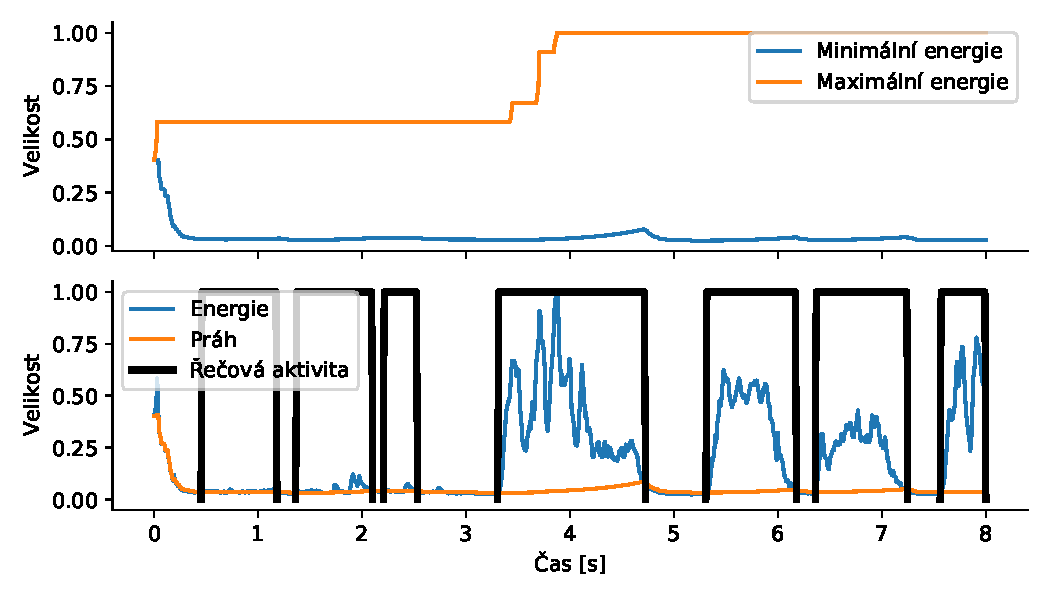
\includegraphics[width=\linewidth]{obrazky-figures/vad_adaptive.pdf}
  \caption{Princip funkcionality adaptivního prahu. Na obrázku je zobrazena energie signálu, její minimální a maximální hodnota příslušných rámců, adaptivní práh a řečová aktivita vyhlazená mediánovým filtrem o~velikosti 20~milisekund.}
  \label{fig:VAD_adaptive_threshold}
\end{figure}


\subsubsection{Gaussovská směsice tří komponent}
\label{subsection:VAD_GMM}
Na rozdíl od algoritmů popsaných v~předchozích sekcích je díky tomuto přístupu možné získat měkká rozhodnutí v~podobě pravděpodobnosti, že se jedná o~řeč, ticho nebo šum. Tyto pravděpodobnosti lze dále vyhladit použitím forward-backward algoritmu nebo jiné filtrační metody. Metoda je založena na směsi tří Gaussovských jednorozměrných rozložení reprezentujících řeč, šum a ticho. Model je trénován na energiích segmentů signálu $\mathbf{E}$ a jeho parametry jsou inicializovány následovně
 

\begin{equation}
    \label{eqn:VAD_GMM_weights}
    \omega_{1} = \omega_{2} = \omega_{3} = \frac{1}{3}
\end{equation}

\begin{equation}
    \label{eqn:VAD_GMM_mean1}
    \mu_{1} = min(\mathbf{E})
\end{equation}

\begin{equation}
    \label{eqn:VAD_GMM_mean2}
    \mu_{2} = mean(\mathbf{E})
\end{equation}

\begin{equation}
    \label{eqn:VAD_GMM_mean3}
    \mu_{3} = max(\mathbf{E})
\end{equation}

\begin{equation}
    \label{eqn:VAD_GMM_sigmas}
    \sigma^2_{1} = \sigma^2_{2} = \sigma^2_{3} = 1
\end{equation}

Parametry Gaussovské směsice dodržují značení definované v~podsekci~\ref{subsection:GMM}. Funkce označena jako $mean(\mathbf{X})$ vrací střední hodnotu položek vektoru $\mathbf{X}$, obdobně $min(\mathbf{X})$ nejmenší položku a $max(\mathbf{X})$ tu největší.

Model je trénován v~několika iteracích dokud není dosažena konvergence. Následně je vypočtena věrohodnost každého segmentu vůči každé komponentě modelu. Takto je získán vektor o~velikosti $3 \times N$, kde $N$ je počet segmentů signálu. Vektor je vyhlazen forward-backward algoritmem s~příslušnou přechodovou maticí.

Posledním krokem je určení řečově aktivních segmentů. Jako aktivní segmenty jsou zvoleny ty, kde je věrohodnost ticha nižší než práh. Aktivní segmenty jsou následně vyhlazeny podle potřeb následného zpracování. \imageref{fig:VAD_GMM}{1} znázorňuje funkcionalitu takového systému.
\begin{figure}[ht]
  \centering
  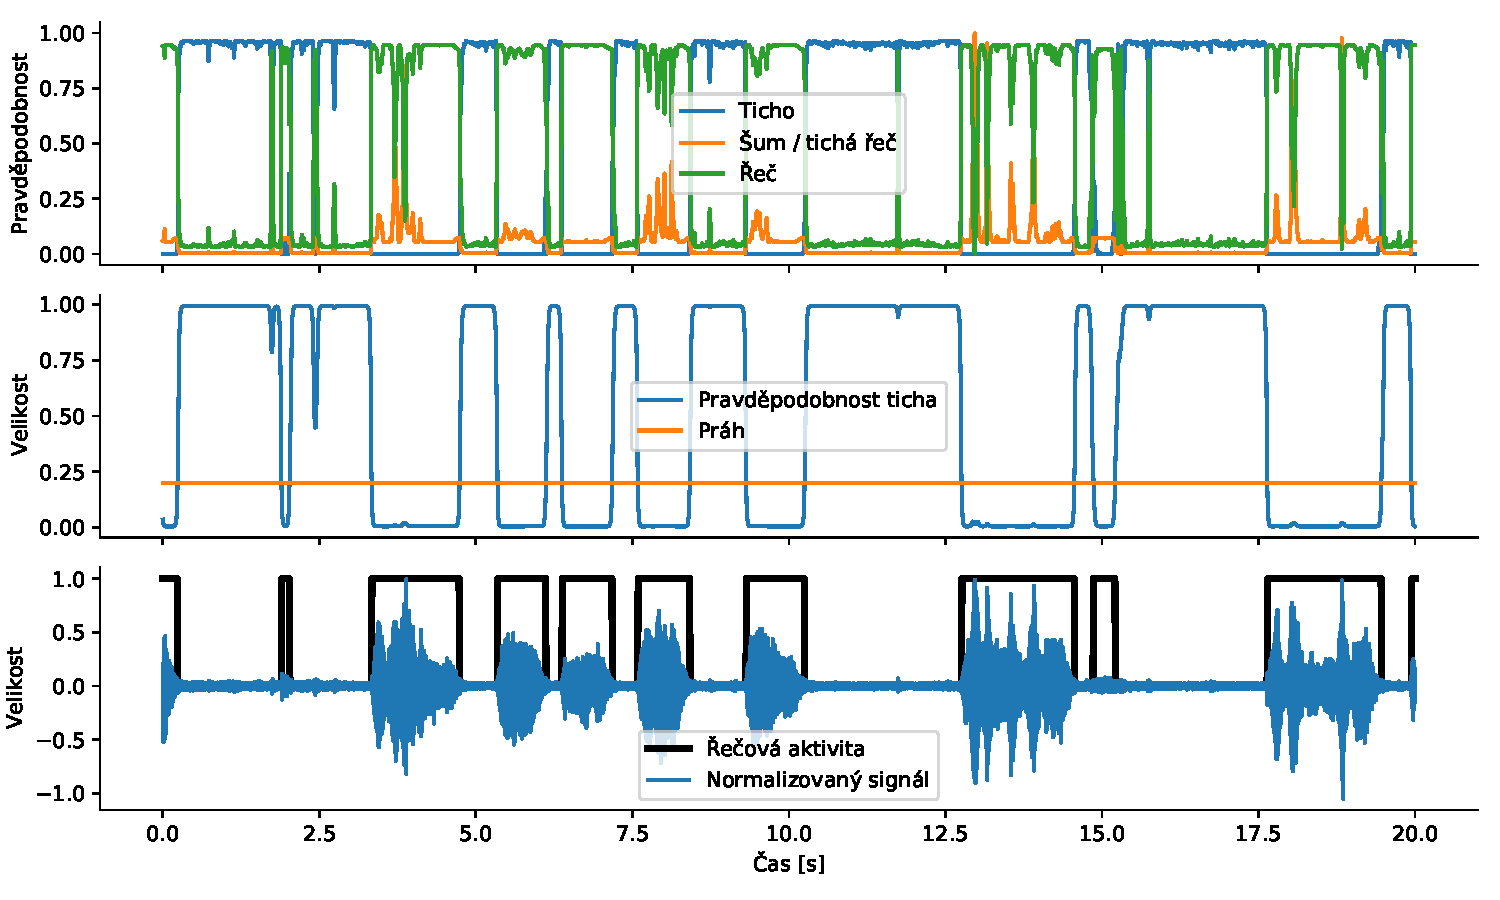
\includegraphics[width=\linewidth]{obrazky-figures/vad_gmm.pdf}
  \caption{Detekce řečové aktivity pomocí směsice Gaussovských rozložení. Na horním obrázku jsou zobrazeny pravděpodobnosti příslušných komponent reprezentujících ticho, šum a řeč. Pravděpodobnosti jsou vyhlazeny forward-backward algoritmem s~příslušnou přechodovou maticí. Tvrdé rozhodnutí o~řečové aktivitě podle věrohodnosti komponenty reprezentující ticho demonstruje obrázek uprostřed. Spodní obrázek zobrazuje detekci řečové aktivity pro systémy velmi citlivé na aktivitu mluvčího.}
  \label{fig:VAD_GMM}
\end{figure}

%%%%%%%%%%%%%%%%%%%%%%%%%%%%%%

\section{Diarizace}
\label{section:Diarization}
Diarizace je proces rozdělení audio nahrávky na homogenní úseky odpovídající příslušným mluvčím. Odpovídá na otázku~\uv{kdo kdy mluví} v~prostředí více mluvčích. Metoda je využívána v~mnoha odvětvích zpracování a následné analýzy řeči. Přesnosti systémů se každým rokem zlepšují a přesnosti komerčně využívaných systémů se blíží ke 100~\%. Správně označené úseky řeči mluvčích vedou k~výraznému zlepšení systémů rozpoznání řeči (ASR -- Automatic speech recognition), tedy systémů tvořících přepis (transkripci) řečových nahrávek. Typický diariya4n9 systém se skládá ze segmentace, extrakce příznaků, shlukování a případně resegmentace. 

\subsubsection{Segmentace} 
Nahrávka se rozdělí do $N$ segmentů o~stejné délce $M$ popsané v~sekci~\ref{subsection:Segmentation}. Ze segmentů jsou dále odfiltrovány ty, které neobsahují řečovou aktivitu podle sekce~\ref{section:VAD}.

\subsubsection{Extrakce příznaků}  
Z~řečově aktivních segmentů jsou extrahovány příznaky. Nejčastěji se jedná o~MFCC příznaky popsané v~podsekci~\ref{subsection:MFCC}, faktory řečníka a jejich vlastní čísla~\cite{Speaker_factors}, i-vektory~\cite{Dehak_i_vectors}, x-vektory~\cite{Snyder_x_vectors} nebo případně d-vektory~\cite{Wang_d_vectors}.

\subsubsection{Shlukování}
Příslušné segmenty signálu jsou přiřazeny řečníkům. Nejčastěji jsou za tímto účelem využity neuronové sítě~\cite{Bishop_pattern} nebo směsi Gaussovských rozložení popsané v~podsekci~\ref{subsection:GMM}.

\subsubsection{Resegmentace}
Podobně jako u~detekce řečové aktivity je vhodné provést vyhlazení výsledků pomocí filtrace nebo forward-backward algoritmu pomocí přechodové matice definující pravděpodobnosti změny řečníků. 

Blokové schéma na~\imageref{fig:Diar_schema}{0} znázorňuje základní architekturu diarizačního systému. \imageref{fig:Diar_smooth}{1} zobrazuje demonstrační výstup diarizačního systému. 

\begin{figure}[ht]
  \centering
  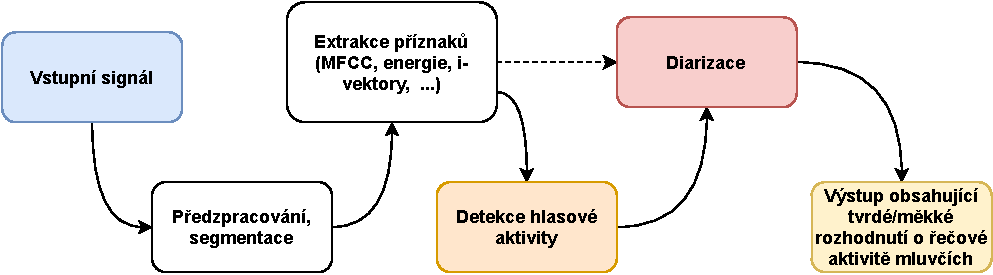
\includegraphics[width=\linewidth]{obrazky-figures/diarization_diagram.pdf}
  \caption{Blokové schéma diarizace.}
  \label{fig:Diar_schema}
\end{figure}

\begin{figure}[ht]
  \centering
  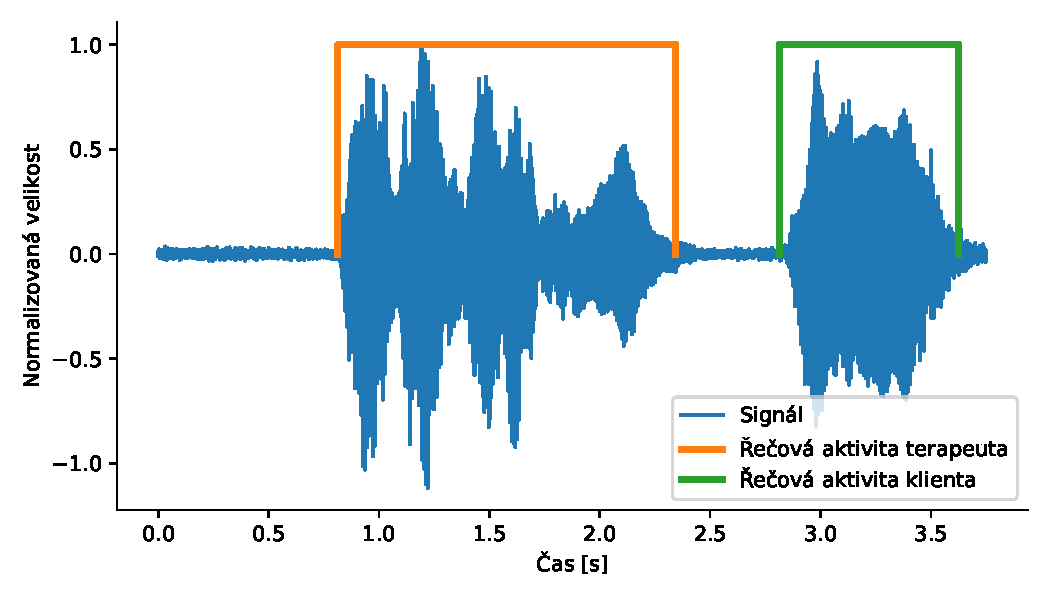
\includegraphics[width=\linewidth]{obrazky-figures/diarization.pdf}
  \caption{Detekce řečové aktivity příslušných řečníků vstupního signálu.}
  \label{fig:Diar_smooth}
\end{figure}

\section{Rozpoznávání řeči}
\label{section:ASR}
Následující sekce vychází z~článku společnosti IBM\cite{asr_ibm}, která je jedním z~vedoucích vývojářů v~oblasti ASR\footnote{Automatic speech recognition} (Automatické zpracování řeči). Automatické rozpoznávání řeči je další ze skupiny metod pro získání informací z~vstupní nahrávky. Rozpoznáváním řeči se rozumí automatický převod mluvené řeči do textu. Získaný text je následně možné dále zpracovávat, analyzovat nebo vytvářet automatické odpovědi v~textové, případně v~hlasové podobě pomoci syntetizátoru řeči. Tímto způsobem dokáže v~dnešní době komunikovat počítač s~člověkem.

Při návrhu systému ASR je nutno dbát na rozdíly v~intonaci, výslovnosti, přízvuku, výšce či hlasitosti mluvčích. Některé metody mohou být velmi citlivé na hluk v~pozadí, který může způsobovat špatné výsledky. Obecně rozlišujeme dva druhy ASR systémů:

\begin{itemize}
    \item závislé na mluvčím (speaker dependent, SD),
    \item na mluvčím nezávislé (speaker independent, SI).
\end{itemize}

Systémy závislé na mluvčím dosahují lepších výsledků, ale jejich nevýhodou je, že mluvčí musí namluvit sadu nahrávek, aby bylo možné natrénovat příslušné modely. Existují však metody, které modely natrénované na velkém počtu mluvčích dokáží adaptovat na konkrétní osobu. Takové systémy můžeme pozorovat ve většině mobilních telefonů v~podobě Asistenta Google\footnote{\url{https://assistant.google.com/}} nebo systému Siri\footnote{\url{https://www.apple.com/siri/}} firmy Apple. Značné využití systémů ASR můžeme sledovat i ve zdravotnictví nebo v~automobilovém průmyslu. 

Rozpoznání řeči je přímo závislé na diarizaci nahrávky. Pomocí skrytých Markových modelů~\cite{Cernocky_ZRE}, N-gramů~\cite{jurafsky_martin_2020} a neuronových sítí~\cite{Bishop_pattern} jsou poté vytvořeny modely pro příslušný jazyk, odvětví.

V~současné době existuje mnoho firem a univerzit vyvíjejících vlastní interní systémy. Některé z~nich jsou poskytnuté v~podobě online rozhraní. Mezi nejznámější patří:

\begin{itemize}
    \item Google Cloud Speech API\footnote{\url{https://cloud.google.com/speech-to-text}}
    \item Microsoft Bing Voice Recognition\footnote{\url{https://azure.microsoft.com/en-us/services/cognitive-services/speech-to-text/}}
    \item IBM Speech to Text\footnote{\url{https://www.ibm.com/cloud/watson-speech-to-text}}
    \item Wit.ai\footnote{\url{https://wit.ai/}}
    \item Houndify API\footnote{\url{https://www.houndify.com/}}
\end{itemize}

Zároveň existuje mnoho volně dostupných systémů, které je možné natrénovat pro individuální účely. Mezi nejznámější patří DeepSpeech\footnote{\url{https://github.com/mozilla/DeepSpeech}} společnosti Mozilla, sada nástrojů Kaldi\footnote{\url{https://github.com/kaldi-asr/kaldi}} nebo starší systém CMUSphinx\footnote{\url{https://cmusphinx.github.io/}}.


%%%%%%%%%%%%%%%%%%%%%%%%%%%%% Data %%%%%%%%%%%%%%%%%%%%%%%%%%%%%

\chapter{Data}
\label{chap:Data}
Automatické zpracování a následná analýza psychoterapeutických sezení vyžaduje databázi dat, vůči kterým je možné příslušná sezení porovnávat a strojově zpracovávat. Při zpracování nahrávek jsou využívány algoritmy strojového učení. Ty v~datech hledají vzory, které dokáží formulovat předpovědi. S~větším množstvím dat a více zkušenostmi jsou výsledky strojového učení přesnější – stejně jako se lidé zlepšují díky větší praxi. Psychoterapie je velmi citlivé odvětví, co se týče ochrany dat a tak neexistují žádné volně dostupné datasety. V~rámci této práce jsou využita data projektu DeePsy\footnote{\url{https://www.deepsy.cz}}, ta však obsahovala v~době psaní této práce nedostatečný počet nahrávek, a byly proto doplněna o~dataset CallHome\footnote{\url{https://catalog.ldc.upenn.edu/LDC97S42}}. Dataset CallHome byl vybrán z~důvodu vysoké podobnosti struktury nahrávek k~nahrávkám online psychoterapeutických sezení projektu DeePsy. V~obou případech obsahují datasety nahrávky rozhovorů dvou osob, které jsou rozděleny do dvou kanálů bez přeslechů.

%%%%%%%%%%%%%%%%%%%%%%%%%%%%%%

\section{CallHome}
Dataset CallHome American English Speech vytvořilo v~roce 1997 mezinárodní konsorcium univerzit, knihoven, společností a vládních výzkumných laboratoří Linguistic Data Consortium\footnote{\url{https://www.ldc.upenn.edu}}. Skládá se ze 120~telefonních~nahrávek rodilých mluvčích v~anglickém jazyce. Délka nahrávek se pohybuje okolo 30~minut a jedná se většinou o~rozhovory mezi členy rodiny nebo rozhovory mezi blízkými přáteli. Vzorkovací frekvence nahrávek je 8~kHz. Dataset se skládá ze stereo nahrávek a jejich transkripcí. Transkripce však nepokrývají celou délku nahrávky a v~této práci byly využity pouze anotované části datasetu, jedná se o~80 souborů o~průměrné délce zhruba 10 minut. Příslušné kanály nahrávky od sebe oddělují mluvčí a neobsahují téměř žádný přeslech. V~některých případech obsahují kanály navíc řečovou aktivitu dalších mluvčích. Většinou se však jedná o~mluvu o~délce jedné věty a pro účely této práce je skupina těchto mluvčích reprezentovaná jedním mluvčím.

%%%%%%%%%%%%%%%%%%%%%%%%%%%%%%

\section{DeePsy}
DeePsy je projekt vedený týmem psychologů a psychoterapeutů z~Masarykovy univerzity a odborníků na informační technologie z~Vysokého učení technického v~Brně. Zkoumají možnosti, jakými mohou informační technologie obohatit a zkvalitnit psychoterapeutickou péči. Na projektu spolupracují Psychosomatická klinika, s.r.o., a Terapeutický přístav, z.ú., kterým účast umožňuje zlepšit kvalitu svých psychoterapeutických služeb. Všichni účastníci poskytují zpětnou vazbu o~sezeních a souhlasí s~jejich nahráváním. Cílem projektu je poskytnout terapeutům zpětnou vazbu a najít potenciálně problematické úseky k~analýze a tím umožnit celkové zkvalitnění poskytované psychoterapeutické péče. Dataset obsahuje anonymizované nahrávky prezenčních a online sezení. Délka psychoterapeutických sezení většinou nepřekračuje 60~minut, obvykle se pohybuje okolo 50~minut.

\subsection{Online sezení}
Online sezení probíhají výhradně na platformě ZOOM\footnote{\url{https://zoom.us/}}. Tato platforma umožňuje stáhnout video/audio záznam ihned po ukončení sezení. Při  správném nastavení aplikace\footnote{\url{https://support.zoom.us/hc/en-us/articles/201362473-Local-recording\#h_96380e17-816d-4eda-a4b9-740d1498eac6}} jsou od sebe odděleny kanály mluvčích. Vzniká tak separátní nahrávka pro každého účastníka sezení, což vede k~vyšší přesnosti diarizace blížící se k~100~\%. Nejlepší výsledky jsou dosaženy na nahrávkách, ve kterých terapeut i klient používají náhlavní sady (sluchátka s~mikrofonem). Takovéto nahrávky neobsahují skoro žádný okolní hluk a jsou ideální pro následné zpracování.

\subsection{Prezenční sezení}
\label{subsection:Data_offline}
Druhá skupina nahrávek je pořizována pomocí diktafonu ZOOM H2n. Diktafon je používán v~režimu 4CH s~maximální citlivostí. Toto nastavení vede k~získání stereo nahrávky sezení, ve které je značně eliminován okolní hluk. Kanály však obsahují značný přeslech, který je demonstrován na~\imageref{fig:Cross-talk}{0}, což vyžaduje náročnější zpracování pro určení, kdy kdo mluví. Pro optimální výsledky je vhodné diktafon umístit ve stejné vzdálenosti mezi terapeutem a klientem, jak znázorňuje \imageref{fig:Dictaphone}{0}. V~opačném případě může být energie jednoho z~řečníků značně vyšší.


\begin{figure}[ht]
\begin{subfigure}{0.65\textwidth}\centering
    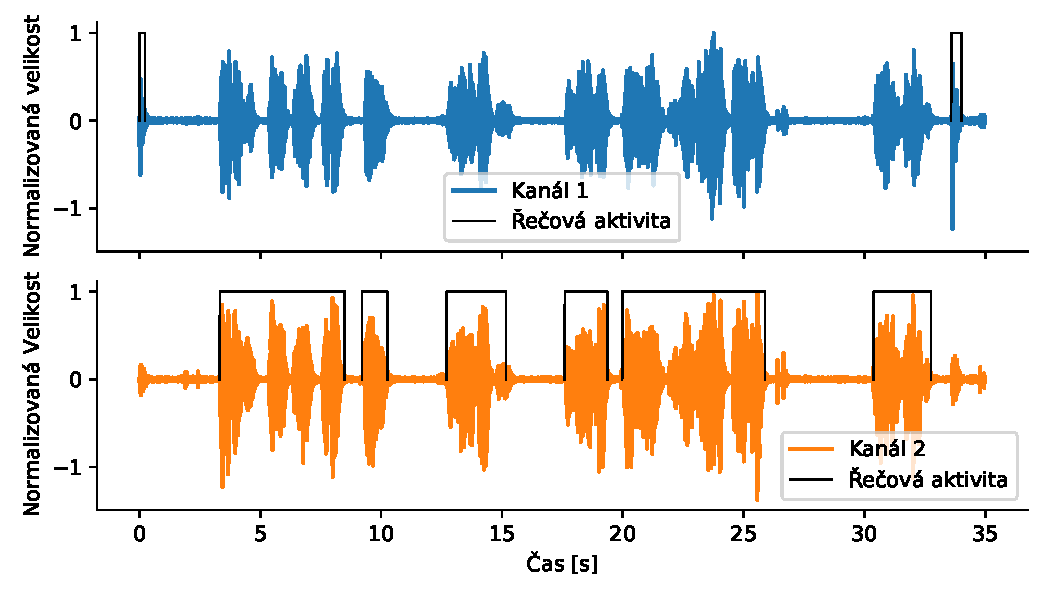
\includegraphics[width=\linewidth]{obrazky-figures/cross_talk.pdf}
    \caption{Přeslech mezi kanály nahrávky. Z~obrázku je patrné, že řečová aktivita mluvčích je zaznamenána v~obou kanálech zdrojové nahrávky. Je tedy nutné provést diarizaci nad vstupní nahrávkou.} \label{fig:Cross-talk}
  \end{subfigure}%
    \hspace*{\fill}
  \begin{subfigure}{0.3\textwidth}
 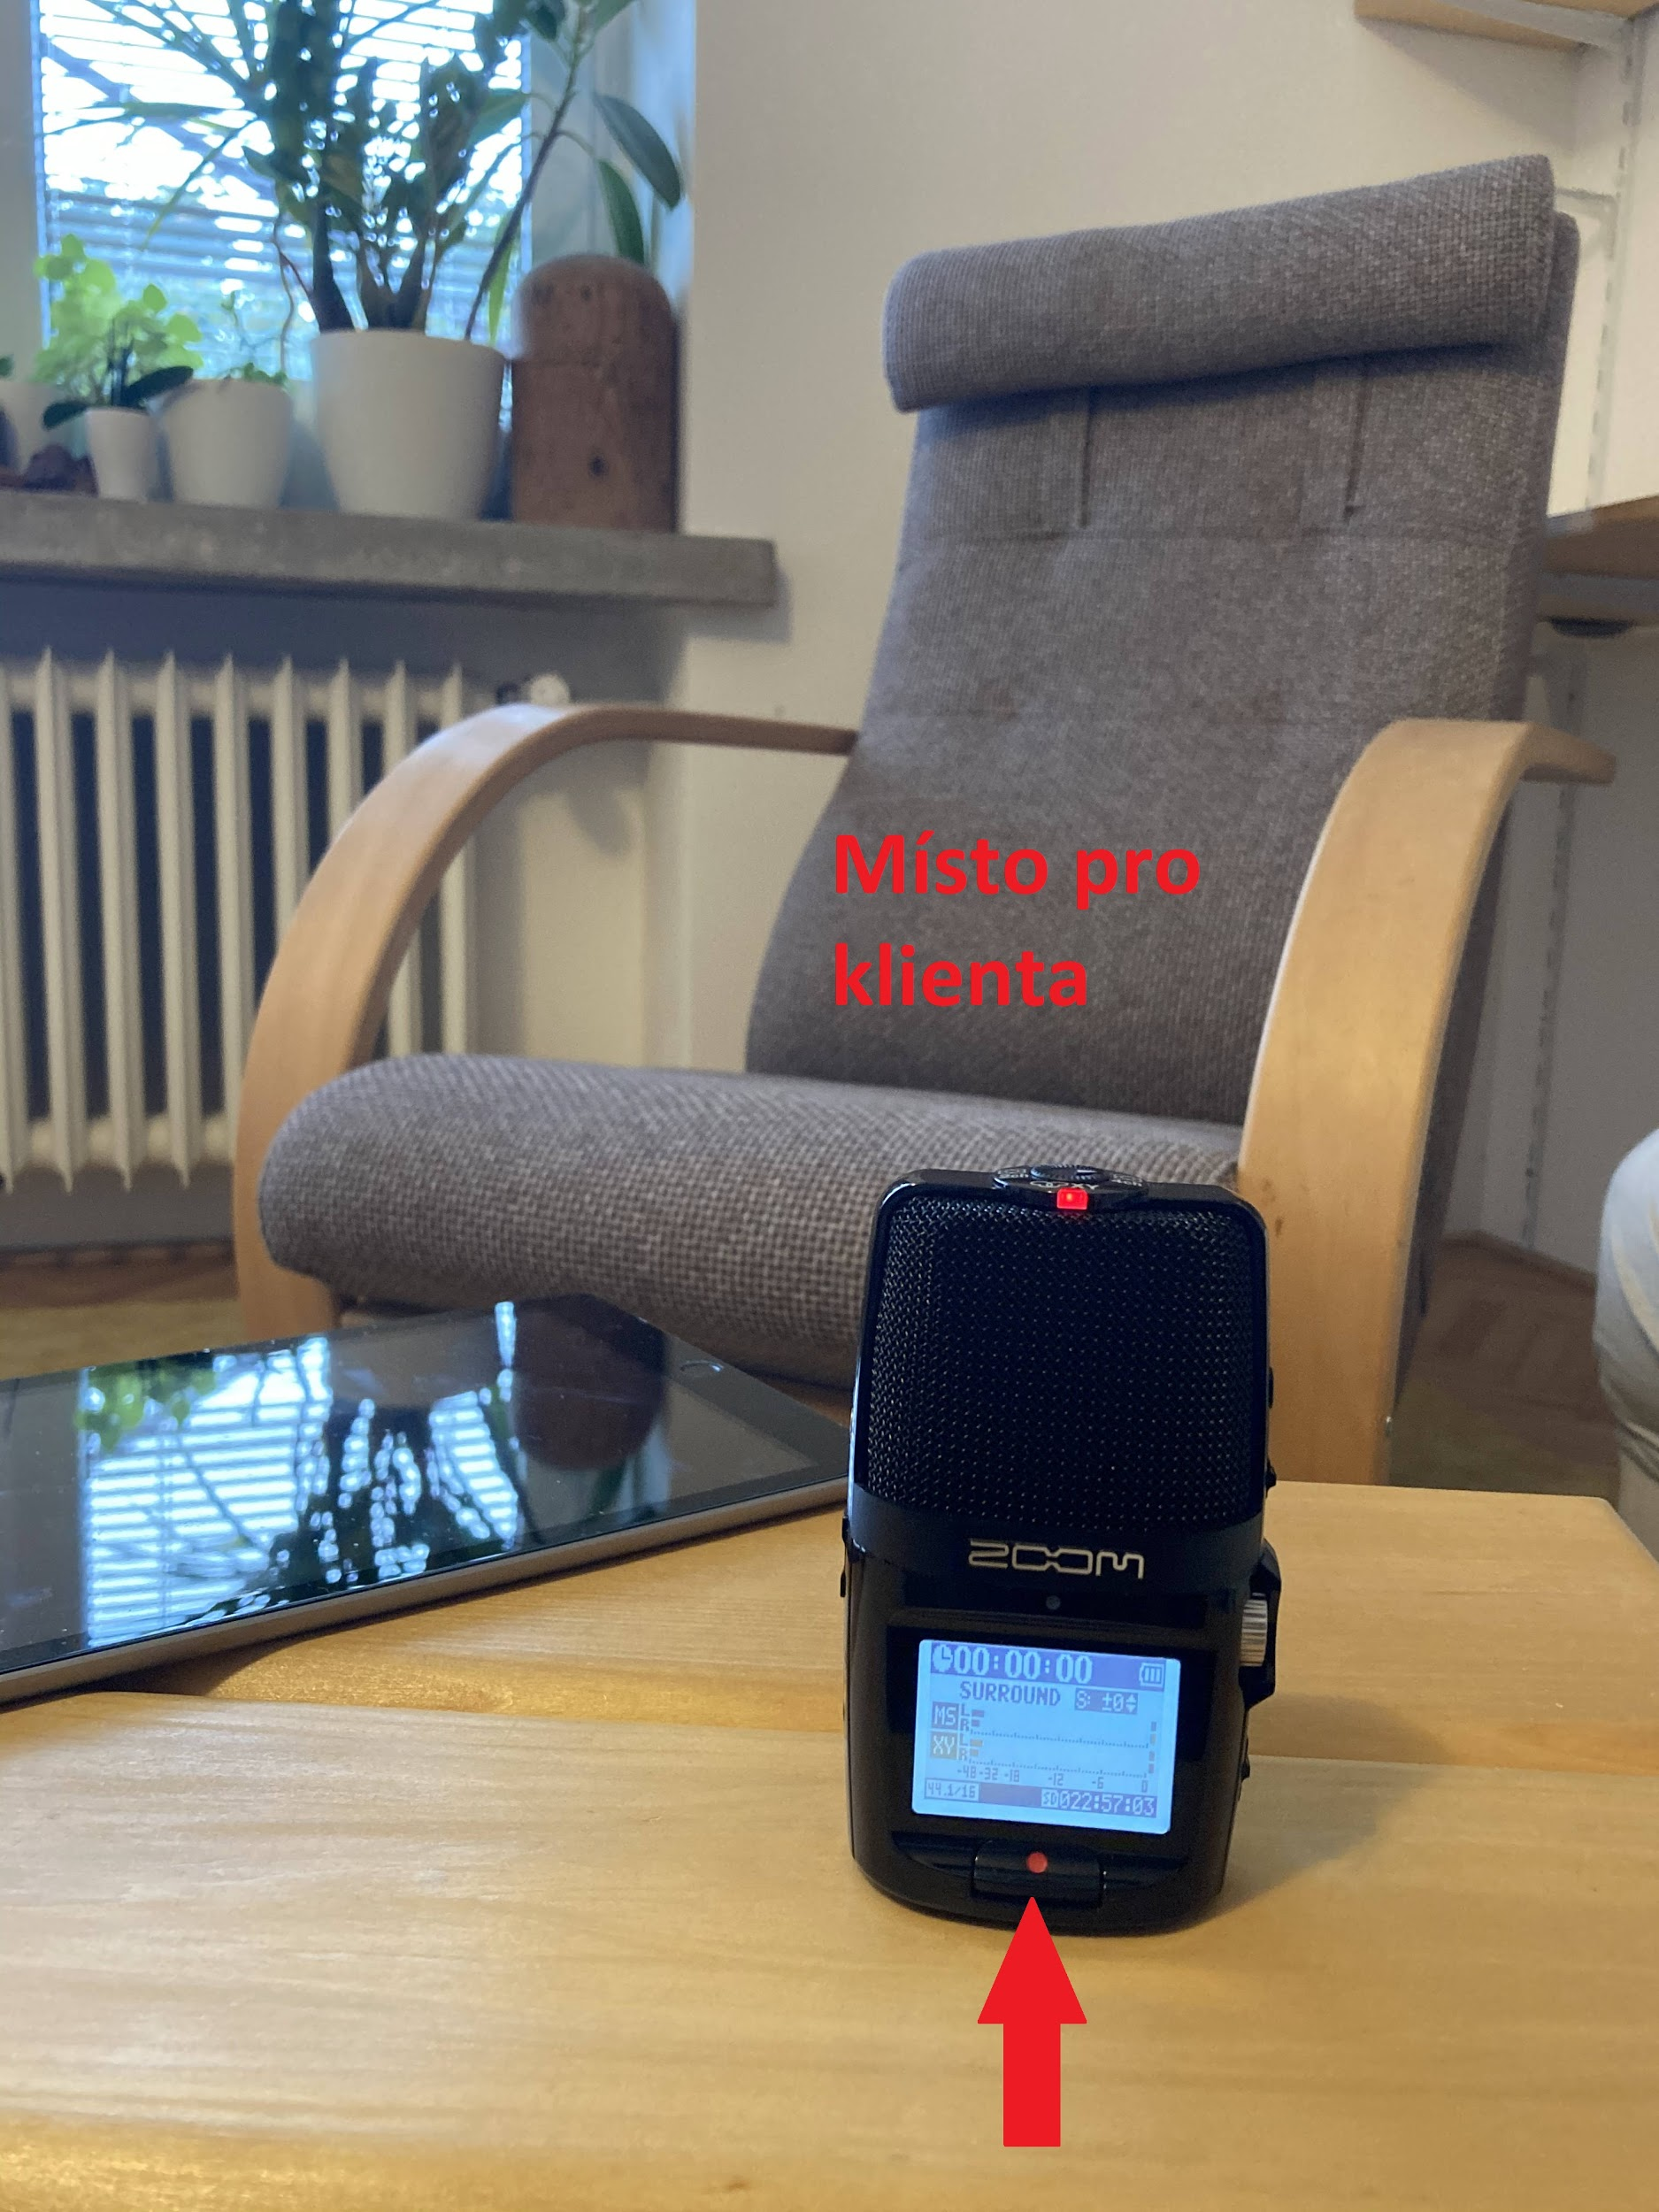
\includegraphics[width=\linewidth]{obrazky-figures/dictaphone.jpg}    \caption{Optimální poloha diktafonu v~průběhu sezení. Červená šipka označuje směr, ze kterého hledí terapeut na diktafon.}          \label{fig:Dictaphone}
  \end{subfigure}
  \caption{Nahrávky pořízené diktafonem ZOOM H2n.}
\end{figure}

%%%%%%%%%%%%%%%%%%%%%%%%%%%%%%

\section{Anotační soubory}
\label{section:Anotation}
Datová sada CallHome obsahuje kromě zvukových souborů taktéž anotační soubory s~přepisem úseku nahrávky ve formátu \texttt{.txt}. Ty jsou použity pro validaci výsledků diarizace a automatického přepisu. Pro účely validace diarizace jsou převedeny do formátu Rich Transcription Time Marked (RTTM)~\cite{Rttm}, pomocí kterého je vyhodnocena přesnost systému. Pro nahrávky projektu DeePsy byly anotace vytvořeny ručně pomocí nástroje Transcriber\footnote{\url{http://trans.sourceforge.net/en/presentation.php}} Ty jsou taktéž převedeny do formátu RTTM. Standardizovaný formát RTTM je znám především díky jeho využití v~soutěžích rozpoznání mluvčích Národního institutu standardů a technologií (NIST)\footnote{\url{https://www.nist.gov}}.

Formát RTTM je definován následujícími poli oddělenými mezerami. Každý řádek popisuje jeden úsek souboru:

\begin{center}
\begin{tabular}{ |c|c|c|c|c|c|c|c|c|c| } 
\hline
1 & 2 & 3 & 4 & 5 & 6 & 7 & 8 & 9 & 10 \\
\hline
Type & File & Channel & Tstart & Tdur & Ortho & Stype & Name & Confidence & Slat \\
\hline
\end{tabular}
\end{center}

Hodnoty polí \textit{Ortho}, \textit{Stype}, \textit{Confidence} a \textit{Slat} obsahují hodnotu \texttt{<NA>} a nejsou pro účely této práce využity. Hodnoty pole \textit{Type} a \textit{Stype} blíže definují původce mluvy nebo řečové aktivity a jsou zde použity konstantní hodnoty \texttt{SPEAKER} a \texttt{<NA>.} Hodnota \textit{File} udává název zdrojového souboru, ke kterému se nahrávka váže (bez přípon a cesty). Pole \textit{Channel} určuje kanál, ke kterému náleží příslušná anotace. \textit{Tstart} určuje začátek řečové aktivity v~sekundách a \textit{Tdur} její délku. Hodnota \textit{Name} obsahuje přidělený identifikátor řečníka.

Následující ukázka představuje dva segmenty řečové aktivity řečníků \texttt{B} a \texttt{A} zdrojového souboru \textbf{en\_4077.wav}. V~nahrávce se nejdříve vyskytuje řečová aktivita řečníka \texttt{B} o~délce 1,55~s. Následuje 20~ms ticha a velmi krátká odpověď o~délce 270~ms. 
\begin{lstlisting}
SPEAKER en_4077 2 0.000 1.550 <NA> <NA> B <NA> <NA>
SPEAKER en_4077 1 1.570 0.270 <NA> <NA> A~<NA> <NA>
\end{lstlisting}


%%%%%%%%%%%%%%%%%%%%%%%%%%%%% Návrh %%%%%%%%%%%%%%%%%%%%%%%%%%%%%

\chapter{Návrh systému}
\label{chap:System_design}
Analýza audio hovoru je velmi rozsáhlý pojem spojený s~řadou technik pro dolování informací z~nahrávky. V~této kapitole je čtenáři postupně představen systém navržený pro analýzu psychoterapeutických sezení. V~sekci~\ref{section:Requirements} jsou sepsány všechny funkcionální požadavky, které by systém pro analýzu citlivých dat, jako jsou nahrávky psychoterapeutických sezení, měl splňovat. V~následující sekci~\ref{section:Architecture} jsou podrobně představeny funkcionální bloky navrženého systému. Systém by měl postupně zpracovávat vstupní nahrávku, extrahovat nezbytné informace a vytvářet souhrnný výstup. Ten je popsán v~sekci~\ref{section:Stats}. Funkcionalitu systému je potřeba validovat. Metriky k~tomu určené jsou popsané v~sekci~\ref{section:Validation}.

%%%%%%%%%%%%%%%%%%%%%%%%%%%%%%

\section{Funkcionální požadavky}
\label{section:Requirements}
Systém pracuje s~daty, která jsou velmi citlivá a jejich únik by mohl být pro uživatele velmi nepříjemný. Z~tohoto důvodu musí být systém schopný provozu výhradně v~\textbf{offline} režimu bez využití jakýchkoliv online nástrojů. Pro zajištění co největší bezpečnosti je taktéž nutné limitovat výstupy systému a to takovým způsobem, že může systém zanechávat soubory a datové výstupy pouze v~místech k~tomu explicitně určených. Pro vyšší \textbf{bezpečnost} je uživateli vřele doporučena anonymizace dat, kterou však systém explicitně nebude zajišťovat.

Jelikož dlouhá doba zpracování může být pro uživatele nepříjemná a poskytnutí zpětné vazby v~době, kdy má terapeut sezení ještě čerstvě v~paměti, může být značně přínosnější, dalším z~požadavků je \textbf{rychlost} zpracování nahrávky. Z~tohoto důvodu musí být \textbf{komplexita} systémů snížena na co nejmenší možnou míru a k~implementaci musí být využity nástroje s~co nejkratší dobu zpracování. Měl by být kladen důraz na \textbf{optimalizaci} příslušných (vysoce náročných) bloků systému.

Příslušné funkcionální bloky popsané v~následující sekci~\ref{section:Architecture} musí fungovat \textbf{odděleně} a musí být možná jejich snadná \textbf{nahraditelnost}. Bloky by měly být navzájem \textbf{nezávislé} a data načítat výhradně ze vstupních souborů a zapisovat do souborů výstupních.

Navržený systém musí extrahovat nejméně \textbf{6 slabých klasifikátorů}, které popisují uskutečněné sezení (např. základní tón řeči, energie, cross-talk, rychlost řeči, poměr řeči, reakční dobu, přepis řeči, sentiment, ...). Ne všechny získané klasifikátory musí být nutně zahrnuty do výstupní souhrnné zprávy.

Výstupní souhrnná zpráva dále popsaná v~sekci~\ref{section:Stats} by měla být v~co nejvyšší míře \textbf{přenositelná}. Z~tohoto důvodu bude využit formát HTML~\cite{Html}, který může být v~průběhu dalšího vývoje doplněn o~elementy uživatelské interakce. Další možnou variantou je PDF\footnote{Portable Document Format} soubor. Ten však nepodporuje elementy interakce v~takové míře jak HTML dokument rozšířený o~kaskádové styly a jazyk Javascript\cite{js} a nebude proto využit.

%%%%%%%%%%%%%%%%%%%%%%%%%%%%%%

\section{Architektura systému}
\label{section:Architecture}
Jak bylo zmíněno v~předchozí sekci, systém je rozdělen na jednotlivé bloky. Ty dovolují postupné zpracování nahrávky po částech. V~rámci spuštění příslušných částí systému je možné zpracovávat více nahrávek najednou. Systém se sestává ze skupiny sedmi funkcionálních bloků, které jsou zodpovědné za:

\begin{itemize}
    \item diarizaci nahrávky online/prezenčního sezení,
    \item evaluaci diarizace (zahrnuje evaluaci detekce řečové aktivity),
    \item tvorbu přepisu z~řečově aktivních úseků,
    \item evaluaci přepisu,
    \item kalkulaci statistik,
    \item kalkulaci celkových statistik všech dostupných nahrávek,
    \item tvorbu souhrnné zprávy příslušné nahrávky.
\end{itemize}

Výše zmíněné bloky je možné vzájemně řetězit. Aby nebyla nutná konverze při načítání a ukládání dat, příslušné bloky sdílejí formát vstupně-výstupních operací a formáty souborů. \imageref{fig:Architecture}{1} zobrazuje architekturu navrženého systému v~podobě diagramu závislostí funkčních bloků a vstupně-výstupních elementů navrženého systému.

Příslušné bloky jsou zároveň navrženy tak, aby v~co nejvyšší míře sdílely společnou funkcionalitu, aby nebyla nutná duplicita kódu. Sdílená funkcionalita je implementována mimo příslušné bloky, aby nedošlo k~neočekávaným změnám funkcionality bloku při modifikaci jiného bloku.

Systém je navržen pro analýzu dat popsaných v~kapitole~\ref{chap:Data} ve formátu WAV (Waveform audio file format). Je schopný pracovat s~libovolnou vzorkovací frekvencí, kterou dynamicky načte, a je možné ho použít pouze pro nahrávky obsahující dva kanály o~celkové délce větší než 1 sekunda.

\begin{figure}[H]
  \centering
  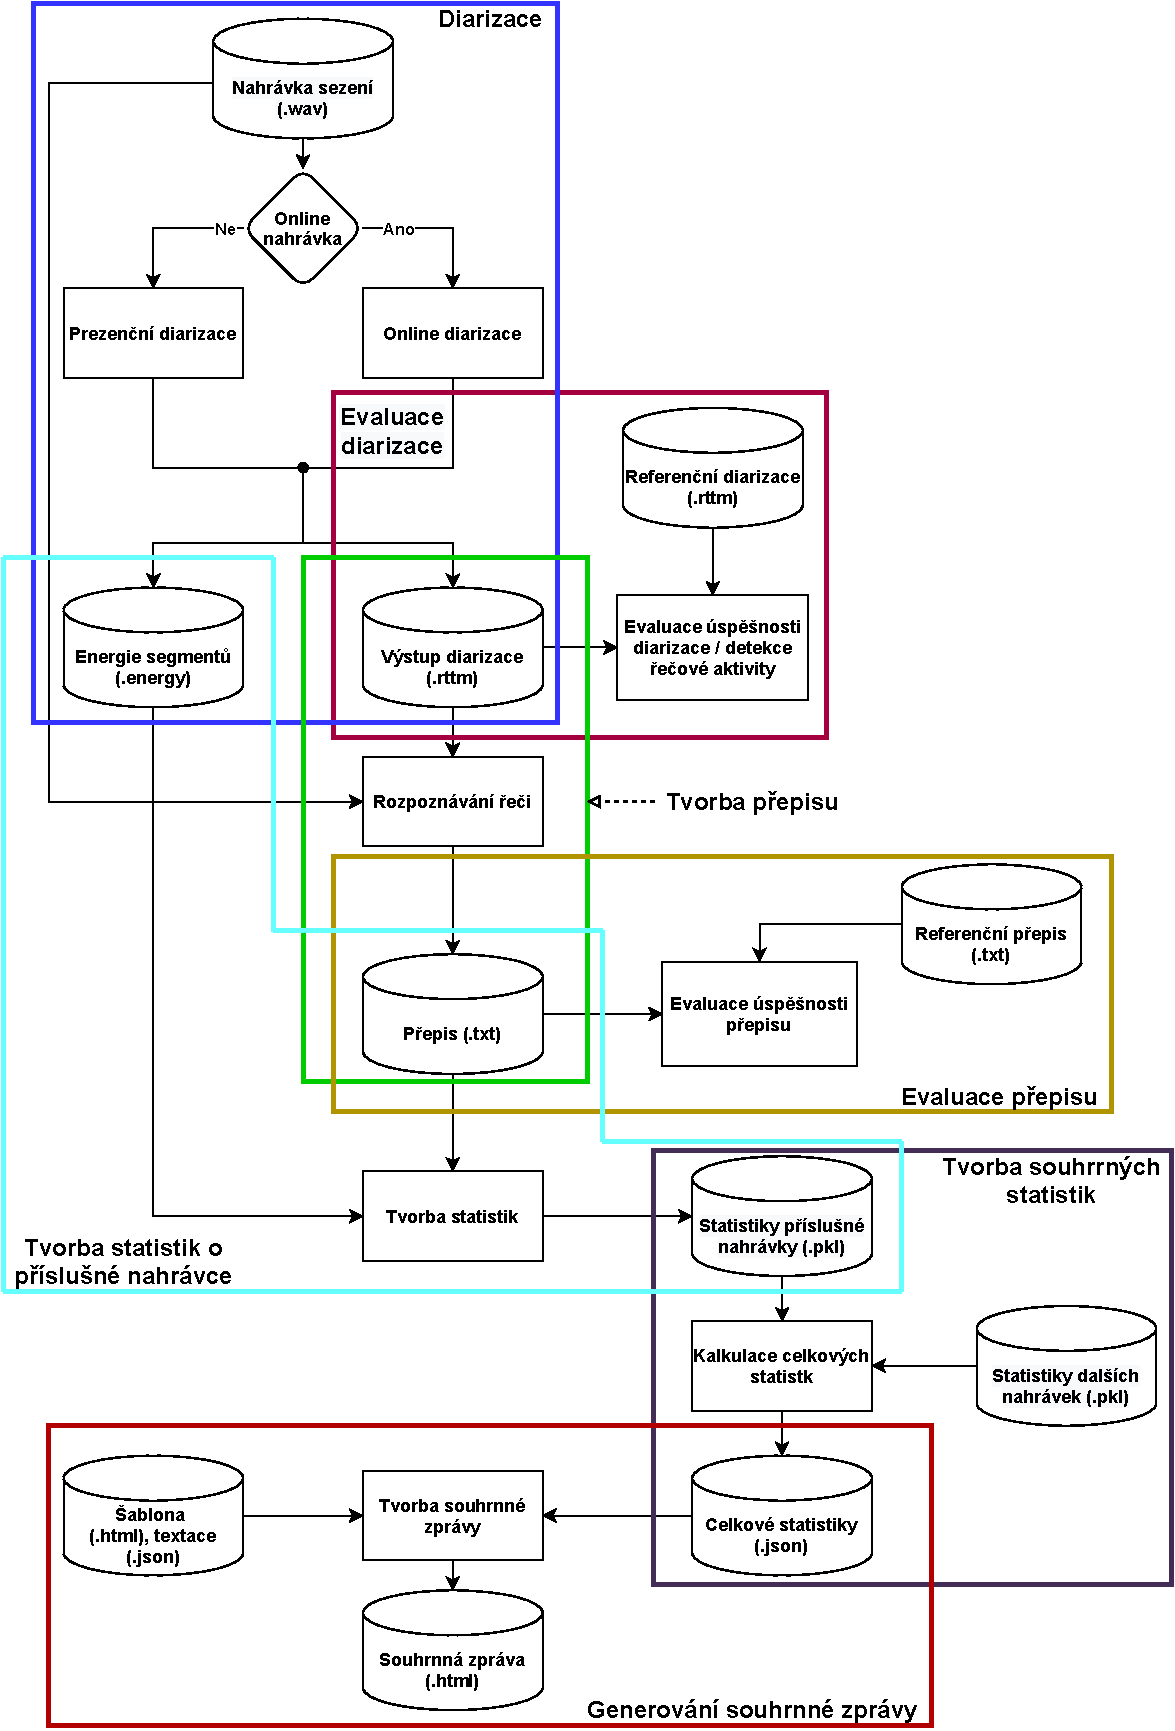
\includegraphics[height=0.9\textheight]{obrazky-figures/system_components.pdf}
  \caption{Diagram architektury systému. Systém se sestává ze skupiny sedmi funkcionálních bloků, které jsou od sebe odděleny barevnými čárami. Navržený systém obsahuje 2 bloky, pomocí kterých je možné validovat výstupy.}
  \label{fig:Architecture}
\end{figure}



\subsection{Parametry}
Zpracování audia a jeho analýza dovoluje použití vysokého počtu parametrů, které vedou k~odlišnému chování systému. Parametry systému se nachází v~jednom sdíleném souboru, a tak není nutné jejich složité dohledávání ve skupině mnoha zdrojových souborů. Návrh předpokládá spuštění celého bloku s~neměnnou konfigurací. Změna parametrů po spuštění jednoho bloku může vést k~zavádějícím výsledkům zpracování v~dalším bloku. Z~tohoto důvodu je nutná konfigurace před spuštěním celého systému nebo opětovné spuštění bloků s~pozměněnými parametry. Nejzajímavější parametry systému a jejich výchozí hodnoty jsou uvedeny v~tabulce~\ref{tab:Params}.

\begin{table}[ht]
\centering
\begin{tabular}{ |c|c|c| } 
\hline
Jméno & Hodnota & Popis \\
\hline
gmm\_components & 32 & \begin{tabular}[c]{@{}c@{}}Počet komponent Gaussovské směsice\\ pro rozpoznání řečníků\end{tabular}   \\
\hline
window\_size & 0,02 & Velikost jednoho segmentu signálu [s] \\
\hline
window\_overlap & 0,01 &  Délka překrytí segmentů [s] \\
\hline
pre\_emphasis\_coefficient & 0,97 &  Koeficient preemfáze \\
\hline
min\_silence\_likelihood & 0,95 &\begin{tabular}[c]{@{}c@{}}Minimální věrohodnost pro\\ klasifikaci segmentu jako ticho\end{tabular}  \\
\hline
\end{tabular}
\caption{\label{tab:Params} Parametry navrženého systému.}
\end{table}

\subsection{Detekce řečové aktivity a diarizace}
\label{subsection:Diar_design}
Systém obsahuje dvě diarizační metody, které jsou optimalizovány pro použití pro příslušný druh psychoterapeutického sezení. Ze vstupní nahrávky s~příponou \texttt{.wav} jsou extrahovány parametry použité pro detekci řečové aktivity a následnou diarizaci.

Obě metody jsou schopné pracovat se třemi detektory řečové aktivity (VAD) založené na energii signálu, jejichž funkcionalita je postupně popsána v~sekci~\ref{section:VAD}. Jako výchozí je použit systém směsice tří Gaussovských rozložení popsaný v~podsekci~\ref{subsection:VAD_GMM}, který byl v~rámci testování (sekce \ref{section:VAD_testing}) vyhodnocen jako nejúspěšnější. Tento systém používá pro rozhodnutí o~řečové aktivitě směsici tří Gaussovských křivek modelujících ticho, šum a řeč. V~následujících matematických výrazech považujme $N$ za počet segmentů kanálu zdrojové nahrávky.

\subsubsection{Online sezení}
V~případě diarizace online nahrávky (nahrávky neobsahující přeslech) je spuštěna detekce řečové aktivity příslušných kanálů nahrávky. Takto je získána matice $\mathbf{V} \in \{ 0,1\} ^{N \times 2}$ booleovských hodnot aktivity segmentů příslušných kanálů. Získanou matici je možné vyhladit, případně odstranit krátkodobé změny řeč/ticho. Vyhlazenou matici $\mathbf{V_{smooth}} \in \{0,1\}^{N \times 2}$ je možné považovat za výstup systému. Na rozdíl od diarizace prezenčního sezení může takto získaný výstup obsahovat úseky, ve kterých je detekována souběžná mluva obou řečníků.

\subsubsection{Prezenční sezení}
Jak již bylo popsáno v~podsekci \ref{subsection:Data_offline} nahrávky prezenčních sezení obsahují značný přeslech mezi kanály. Z~tohoto důvodu není možná jednoduchá diarizace pomocí výstupu řečové aktivity příslušných kanálů a po zvážení všech okolností vzniku nahrávky jsem navrhl čtyři metody, pomocí kterých je možno rozhodnout, který z~řečníků aktuálně mluví. Příslušné metody jsou vyhodnoceny v~kapitole \ref{chap:Evaluation}.

Prvním krokem použitých diarizačních metod je rozhodnutí o~řečové aktivitě příslušného segmentu. Nad kanály nahrávky je spuštěna detekce řečové aktivity. Tím je získána matice $\mathbf{V} \in \{0,1\}^{N \times 2}$ booleovských hodnot aktivity segmentů příslušných kanálů. Následně je provedena logická disjunkce (or) segmentů mezi kanály. Takto je získán vektor $\mathbf{u} \in\{0,1\}^{N}$ booleovských hodnot označující přítomnost řečové aktivity alespoň jednoho z~mluvčích daného segmentu.

\begin{equation}
\label{eqn:VAD}
    u_{n} = V_{n}^{1} \lor V^{2}_{n}, n \in \{1,\dots, N\}
\end{equation}

Zbývá rozhodnout, kdo je původcem mluvy. Příslušné metody se v~tomto aspektu liší a jejich funkcionalita je popsána v~následujících bodech. Všechny metody však na výstupu vracejí vektor $\mathbf{d} \in \{0,1,2\}^{N}$. Příslušné hodnoty znamenají: 
\begin{itemize}
    \item \textbf{0} -- ticho,
    \item \textbf{1} -- mluví řečník reprezentující kanál 1 (terapeut),
    \item \textbf{2} -- mluví řečník reprezentující kanál 2 (klient).
\end{itemize}

Vektor \textbf{d} je po skončení diarizace možné vyhladit odstraněním krátkodobých změn řečníků. \textit{Kanál 1} u~všech typů diarizace (prezenční, online) odpovídá řečové nahrávce mluvy terapeuta. V~případě, že jsou kanály prohozeny, výstup systému není možné považovat za validní.

\begin{enumerate}
    \item \textbf{Energetická diarizace} -- Vstupem je matice energií segmentů $\mathbf{E} \in \mathbb{R}^{N \times 2}$ a vektor řečově aktivních segmentů $\mathbf{u} \in \{0,1\}^{N}$.
    
    Výstupní vektor $\mathbf{d} \in \{0,1,2\}^{N}$ je vytvořen následujícím způsobem podle hodnoty segmentu v~poli \textbf{u} a matici \textbf{E}.
    
    \begin{equation}
    \label{eqn:DIAR_energy_active}
        d_{n} = \begin{cases}
            0               & u_{n} = 0\\
            1         & E_{n}^{1} > E_{n}^{2}\\
            2         & jinak\\
                        \end{cases}, n \in \{1,\dots, N\}
    \end{equation}
    
    \item \textbf{Mel-frekvenční diarizace s~využitím jednoho kanálu} -- Obdobně jako u~předchozí metody je vstupem matice energií segmentů $\mathbf{E} \in \mathbb{R}^{N \times 2}$, vektor řečově aktivních segmentů $\mathbf{u} \in \{0,1\}^{N}$ a navíc tenzor Mel-frekvenčních cepstrálních koeficientů $\mathbf{M} \in \mathbb{R}^{N \times K \times 2}$, kde $K$ je počet koeficientů segmentu určený nastavitelným parametrem v~konfiguračním souboru.
    
    Z~vstupního tenzoru $\mathbf{M}$ jsou extrahovány segmenty, ve kterých se vyskytuje řečová aktivita jednoho z~kanálu. Dimenzionalita nově vzniklého tenzoru $\mathbf{F}$ je rovna $A \times K$, kde $A = \sum_{n=1}^{N} u_{n}$. 
    
    S~takto získaným tenzorem $\mathbf{F}$ je natrénována směsice Gaussovských rozložení (GMM) blíže popsaná v~sekci \ref{subsection:GMM}. Počet komponent $C$, konvergenční práh a maximální počet iterací je opět nastavitelný v~konfiguračním souboru. Jelikož v~této úloze nelze předpokládat korelaci mezi Mel-frekvenčními cepstrálními koeficienty, je využita diagonální kovarianční matice pro optimalizační účely. Následně je proveden výpočet rozdílů energií segmentů příslušných kanálů, čímž vzniká vektor $\mathbf{e}_{d}$.
    
    \begin{equation}
    \label{eqn:Energy_diff}
       \mathbf{e}_{d} = \mathbf{E}^{1} - \mathbf{E}^{2}
    \end{equation}
    
    Z~natrénovaného univerzálního modelu $\mathtt{G}$ jsou vytvořeny dvě kopie -- $\mathtt{G}^{1}$ reprezentující terapeuta a $\mathtt{G}^{2}$ reprezentující klienta. Z~tenzoru $\mathbf{F}$ je extrahováno $X$~\% nejkladnějších segmentů vektoru $\mathbf{e}_{d}$, čímž vzniká tenzor $\mathbf{S} \in \mathbb{R}^{A/5 \times K \times 2}$ a $X$~\% nejzápornějších segmentů vektoru $\mathbf{e}_{d}$, které vedou k~vzniku tenzoru $\mathbf{T} \in \mathbb{R}^{A/5 \times K \times 2}$. $X$ označuje zvolený percentil, který by neměl překročit hodnotu 50~\%, v~této práci byly dosaženy nejlepší výsledky s~$X \in \langle 0;10\rangle$. Maximální hodnota percentilu je stanovena na 10~\%, neboť poměr řeči hovořících může být v~daných sezeních značně nevyrovnaný a mohlo by tak docházet k~velké chybovosti. 
    
    Nad nově vzniklým tenzorem $\mathbf{S}$ je proveden jeden krok EM algoritmu vycházející z~modelu $\mathtt{G}$. Z~nové matice věrohodnosti příslušných segmentů $\text{\boldmath$\Gamma$}$ vůči příslušným komponentám jsou vypočteny nové střední hodnoty $\text{\boldmath$\mu$}$. Ty jsou normalizovány sumou věrohodností příslušných komponent $\text{\boldmath$\gamma'$} \in \mathbb{R}^{C}$ modelu $\mathtt{G}$, čímž vzniká nový vektor $\text{\boldmath$\mu'$} \in \mathbb{R}^{C}$.
    
    \begin{equation}
    \label{eqn:Gamma_sum}
       \gamma'_{c} = \sum_{a=1}^{A} \Gamma_{a c} , c \in \{1, \dots, C\}
    \end{equation}
    
    \begin{equation}
    \label{eqn:New_means}
         \text{\boldmath$\mu'$}= \text{\boldmath$\mu$} \times  \text{\boldmath$\gamma'$}^{-1}
    \end{equation}

    Nové váhy komponent $\mathbf{w} \in \mathbb{R}^{C}$ jsou vypočteny následovně:
     
    \begin{equation}
    \label{eqn:New_weights}
        \mathbf{w} = \text{\boldmath$\gamma'$} \times \frac{1}{A}.
    \end{equation}
     
     Z~nových vah $\mathbf{w}$ je vypočten vektor posunu $\mathbf{p}$ podle vztahu:
    
    \begin{equation}
    \label{eqn:Shift_vector}
        \mathbf{p} = P \times \mathbf{w},
    \end{equation}
    
    kde $P$ je parametr posunu, který je vhodné nastavit v~rozmezí 0-5 \%.
    
    Nové střední hodnoty $\text{\boldmath$\mu$}^{1}$  modelu $\mathtt{G}^{1}$ jsou vypočteny následovně:
    
    \begin{equation}
    \label{eqn:New_model_means}
        \text{\boldmath$\mu$}^{1} = (1 - \mathbf{p}) \times \text{\boldmath$\mu$} + \mathbf{p} \times \text{\boldmath$\mu'$}.
    \end{equation}
    
    Nové střední hodnoty $\text{\boldmath$\mu$}^{2}$ modelu $\mathtt{G}^{2}$ jsou vypočteny totožným způsobem nad matici $\mathbf{T}$. \imageref{fig:Center_actualization}{1} demonstruje posun středních hodnot GMM modelující 2-dimenzionální data.
    
    
    \begin{figure}[ht]
      \centering
      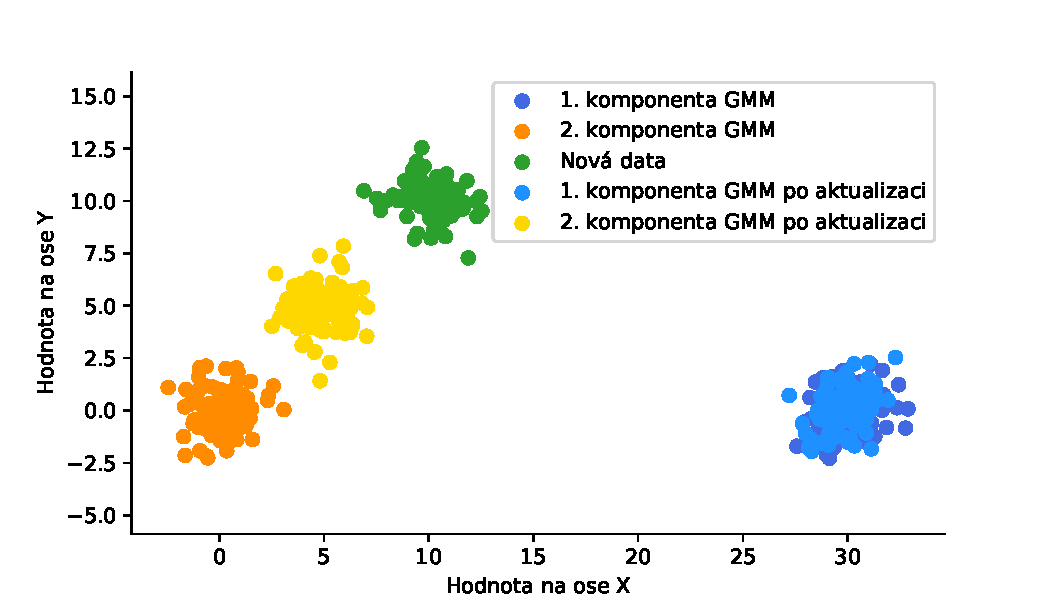
\includegraphics[width=\textwidth]{obrazky-figures/gmm_update.pdf}
      \caption{Aktualizace středních hodnot 2-rozměrné směsice Gaussovských komponent s~parametrem posunu $P = 0,5$.}
      \label{fig:Center_actualization}
    \end{figure}
    
    Následně je vypočtena věrohodnost MFCC koeficientů příslušného segmentu tenzoru \textbf{M} vůči modelu $\mathtt{G}^{1}$ a $\mathtt{G}^{2}$, čímž vznikají vektor $\mathbf{p}^{1} \in \mathbb{R}^{N}$ a $\mathbf{p}^{2} \in \mathbb{R}^{N}$. Jelikož je velmi nepravděpodobná změna mluvčího o~délce několika milisekund uprostřed souvislé několikasekundové promluvy druhého mluvčího, je vhodné nad těmito vektory provést forward-backward algoritmus, pomocí kterého jsou vyhlazeny krátkodobé změny mluvčích. 
    
    Následně je vypočten vektor rozdílu $\mathbf{r}$ věrohodností segmentů $\mathbf{p}^{1}$ a $\mathbf{p}^{2}$.
    \begin{equation}
        \mathbf{r} = \mathbf{p}^{1} - \mathbf{p}^{2}
    \end{equation}
    
    Výsledný vektor \textbf{d} je vytvořen podle následujícího vztahu:
    
    \begin{equation}
    \label{eqn:DIAR_MFCC_1_channel}
        d_{n} = \begin{cases}
            0               & u_{n} = 0\\
            1          & r_{n} > 0\\
            2          & jinak\\
                \end{cases}, n \in \{1,\dots, N\}
    \end{equation}
    
    
    \item \textbf{Mel-frekvenční diarizace s~využitím obou kanálů} -- Tato metoda funguje téměř identicky s~tím rozdílem, že namísto vytvoření tenzoru $\mathbf{F}$ obsahující MFCC aktivních segmentů kanálu 1, je tenzor $\mathbf{F}$ vytvořen spojením řečově aktivních MFCC koeficientů kanálu 1 a 2. Dimenzionalita nově vzniklého tenzoru $\mathbf{F}$ je rovna $A \times 2K$. Zbytek metody je již totožný.
    
    \item \textbf{Mel-frekvenční diarizace ve dvou iteracích s~využitím obou kanálů} -- Následující metoda se značně neliší oproti metodě popsané výše. K~rozdílnému chování dochází po vytvoření vektorů $\mathbf{p}^{1}$ a $\mathbf{p}^{2}$. Pomocí těchto vektorů je vytvořen nový tenzor $\mathbf{S'}$ a $\mathbf{T'}$. Tenzor $\mathbf{S'}$ obsahuje 20 \% nejvěrohodnějších segmentů vektoru $\mathbf{p}^{1}$ tenzoru $\mathbf{F}^{1}$ a obdobně tenzor $\mathbf{T'}$ obsahuje 20 \% nejvěrohodnějších segmentů vektoru $\mathbf{p}^{2}$ tenzoru $\mathbf{F}^{2}$. Následně dochází k~dalšímu posunutí středních hodnot směsic blíže ke středním hodnotám MFCC příznaků extrahovaných tenzorů. Takto by bylo možné vykonat i vícero iterací, dosažené výsledky však neprokazovaly po více iteracích vyšší přesnost.
\end{enumerate}

V~rámci obou navržených podsystémů je po skončení diarizace energie signálu uložena do výstupního souboru s~příponou \texttt{.energy} a výstup diarizace  do souboru s~příponou \texttt{.rttm}, jehož formát je detailněji popsán v~předchozí kapitole v~sekci~\ref{section:Anotation}. 

\subsection{Přepis}
Automatický přepis nahrávek je možný až po provedení diarizace a je tak přímo závislý na předchozím bloku. Aby nebylo nutné znovu spouštět diarizaci, soubory s~příponou \texttt{.rttm} jsou postupně načteny a následně je vytvořen přepis pro řečově aktivní úseky nahrávky. Ten je uložen do souboru s~příponou \texttt{.txt}. Jelikož systém neobsahuje vlastní řešení rozpoznávání řeči a jsou využity externí řešení, byla tato část systému navržena za účelem co možná nejjednodušší záměny ASR modulu v~budoucnosti. Pro nahrávky datasetu CallHome, ve kterých mluvčí hovoří anglickým jazykem, jsou k~dispozici moduly CMUSphinx a Google Cloud Api. Nahrávky projektu Deepsy jsou velmi citlivé a jejich přepis je proveden interním ASR systémem pro český jazyk skupiny Speech@fit\footnote{\url{https://speech.fit.vutbr.cz/}}~\cite{ASR_FIT}. 

Ze vstupní nahrávky jsou postupně extrahovány úseky odpovídající řečové aktivitě příslušného kanálu. Nad každým úsekem je spuštěno rozpoznání řeči a výsledný text je uložen do výstupního souboru.

\subsection{Získání statistik}
S~dostupnými soubory \texttt{.rttm}, \texttt{.txt} a \texttt{.energy} je již možné provést kalkulaci statistik příslušné nahrávky. Sledované statistiky jsou detailně popsány v~následující sekci~\ref{section:Stats}. Tyto hodnoty jsou uloženy pomocí vysokoúrovňového binárního serializačního protokolu pickle~\cite{Pickle} do souboru s~příponou \texttt{.pkl}, aby je bylo možné načíst bez nutnosti manuální serializace.

Z~existujících souborů obsahujících statistiky s~příponou \texttt{.pkl} o~daných sezeních je následně možné vytvořit pomocí dalšího funkcionálního bloku soubor obsahující průměrnou hodnotu sledovaných statistik a jejich varianci mezi nahrávkami. Aby bylo možné do souboru nahlédnout a tyto statistiky interpretovat, jsou hodnoty uloženy ve formátu JSON~\cite{json} s~příponou \texttt{.json}.

\subsection{Generování souhrnné zprávy}
S~využitím souboru obsahujícího textace s~příponou \texttt{.json} a HTML šablonou s~příponou \texttt{.html} (název souboru popisujícího kaskádové styly šablony by měl být pojmenován totožně jako HTML šablona a měl by být ukončen příponou \texttt{.css}) je možné ze získaných statistik vytvořit souhrnnou zprávu s~příponou \texttt{.html} popsanou v~následující sekci \ref{section:Stats}. Všechny výše zmíněné výstupní soubory jsou pojmenovávány podle identifikátoru vstupní nahrávky. Jelikož souhrnná zpráva obsahuje vysoký počet grafů, jsou vygenerované obrázky uloženy v~externí složce vytvořené až za běhu, která je určená uživatelem. 



%%%%%%%%%%%%%%%%%%%%%%%%%%%%%
\section{Dokument shrnující proběhlé sezení}
\label{section:Stats}
Ač to není na první pohled patrné, audio nahrávky obsahují enormní množství informací. Cílem této sekce je vytvořit souhrnnou zprávu obsahující klasifikátory, které jsou pro účely psychoterapie nejzajímavější. V~souhrnné zprávě jsou tyto klasifikátory představeny v~podobě tabulek a grafů tak, aby bylo na první pohled patrné, co příslušné hodnoty představují, jak se sledovaná hodnota mění v~průběhu sezení nebo jak se hodnota liší mezi sezeními. Systém všechny grafy automaticky generuje do předem určené složky podle daného identifikátoru nahrávky, texty obsahující další informace o~sezení jsou taktéž automaticky generované za běhu. Aby nebylo nutné při každém spuštění pracně generovat HTML dokument a aby jeho editace byla co nejpříjemnější, je vytvořena šablona zprávy. Definuje vzhled a obsah souhrnné zprávy. V~rámci tvorby výstupu pro příslušnou nahrávku jsou do kopie šablony dogenerovány nové grafy a doplněny hodnoty spolu s~příslušnými texty. Předdefinovaná šablona taktéž dovoluje značně jednodušší úpravu pro konkretní účely. Její strukturu a vzhled je možné měnit bez zásahů do zdrojových kódů. Je však nutné dodržet pojmenování elementů ve zdrojových kódech i v~šabloně, aby byla na správné místo dosazena správná hodnota. Tento dokument může terapeutovi pomoct odhalit souvislosti, které nemusí být na první pohled patrné. Náhled souhrnné zprávy se nachází v~příloze~\ref{chap:Output_preview}. 

Zkoumáním zvukové stránky verbální komunikace se zabývá věda známá jako Paralingvistika~\cite{krivohlavy}. Vlastnosti řeči mohou být v~průběhu rozhovoru pozměňovány vědomě i nevědomě. V~následujících podsekcích jsou představeny paralingvistické charakteristiky řeči.

%%%%%%%%%%%%%%%%%%%%%%%%%%%%%%

\subsection{Hlasitost}
Hlas netlumočí jen obsah sdělení, nýbrž vypovídá i o~psychickém rozpoložení hovořící postavy. Tento psychický stav se odráží především v~tónu řeči a hlasitosti slovního projevu. U~pacientů trpících bipolární poruchou~\cite{bipolar} lze snadno rozlišit, v~jakém aktuálním stavu se pacient nachází – smutek, skleslost během depresivní polohy či naopak živost a vzrušení při fázi manické. Obdobně lze v~mírnějších podobách tyto aspekty zaznamenat i u~osob bez vážnějších psychických potíží~\cite{krivohlavy}. Terapeut se během terapie zaměřuje na mnoho věcí a změny hlasitosti mu mohou v~průběhu sezení uniknout. Cílem je poskytnout terapeutovi tuto informaci strojově. Je k~tomu využita energie signálu (podsekce~\ref{subsection:Energy}), která je průměrována mezi $N$ sousedními segmenty. Výstup, který je terapeutovi prezentován, je zobrazen na~\imageref{fig:Statisctics_loudness}{0}.

\begin{figure}[ht]
  \centering
  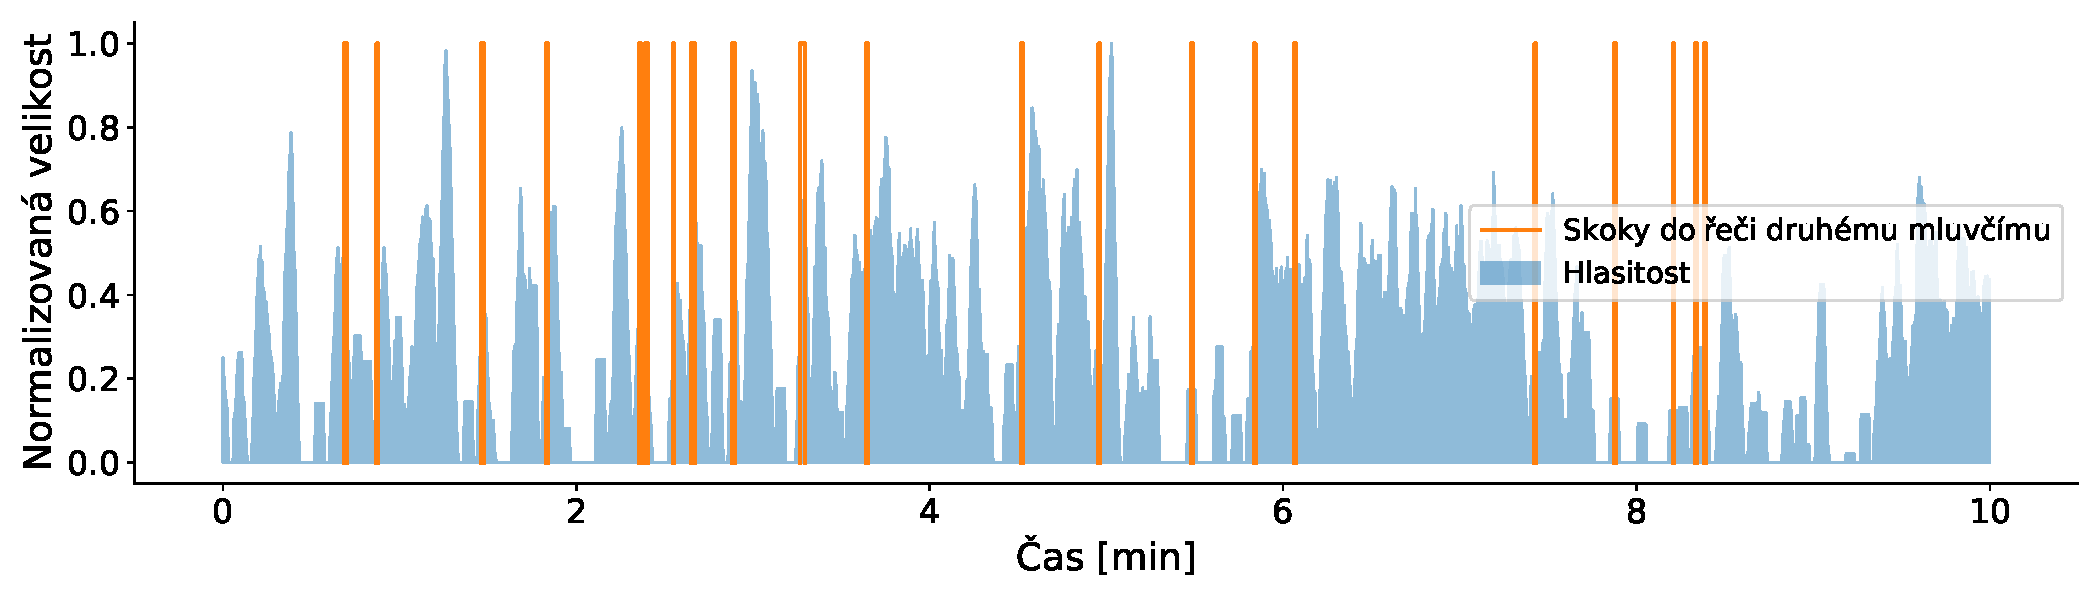
\includegraphics[width=\linewidth]{obrazky-figures/text_plots/therapist_volume.pdf}
  \caption{Měnící se hlasitost v~průběhu sezení. Hlasitost úseků, ve kterých se nenachází řečová aktivita je rovná nule. Nejvyšší hodnoty se nacházejí mezi 4--6~minutou sezení.}
  \label{fig:Statisctics_loudness}
\end{figure}

%%%%%%%%%%%%%%%%%%%%%%%%%%%%%%

\subsection{Poměr řeči}
Mezi další paralingvistické charakteristiky řeči náleží poměr řeči. Prozrazuje nám, kolik toho daný mluvčí řekl v~rámci rozhovoru. Poměr řeči můžeme klasifikovat do tří kategorií charakterizujících dané sezení.
\begin{itemize}
    \item Terapeut vede sezení a klient stručně odpovídá. 
    \item Poměr řeči mezi terapeutem a klientem je vyrovnaný.
    \item Klient vypráví o~nastalé situaci a terapeut naslouchá a klade krátké otázky, které vedou klienta k~rozvinutí dané myšlenky.
\end{itemize}

Terapeutovi je poskytnut poměr řeči mezi ním a klientem a poměr řeči a ticha obou účastníků sezení v~podobě kruhových grafů~\cite{Visualization_pie}. Je mu taktéž poskytnuto porovnání s~ostatními sezeními v~podobě \uv{rychloměru}~\cite{ibm_gauge}, aby byl na první pohled patrný vztah mezi sledovanými veličinami. \imageref{fig:Statisctics_ratio}{1} znázorňuje demonstrační výstup.

Dále můžeme zkoumat, jaký informační objem posluchač doopravdy získal z~přednesu mluvčího. Tuto informaci lze orientačně získat pomocí odstranění spojek, předložek, částic a obdobných slov z~přepisu nahrávky a vydělení délkou příslušných úseků mluvy. V~průběhu psychoterapeutického sezení tyto hodnoty mohou značně kolísat a nepřinášejí terapeutovi až tak zásadní zjištění, a proto nejsou zahrnuty do souhrnného výstupu.

\begin{figure}[ht]
    \begin{subfigure}{0.5\textwidth}
        \centering
        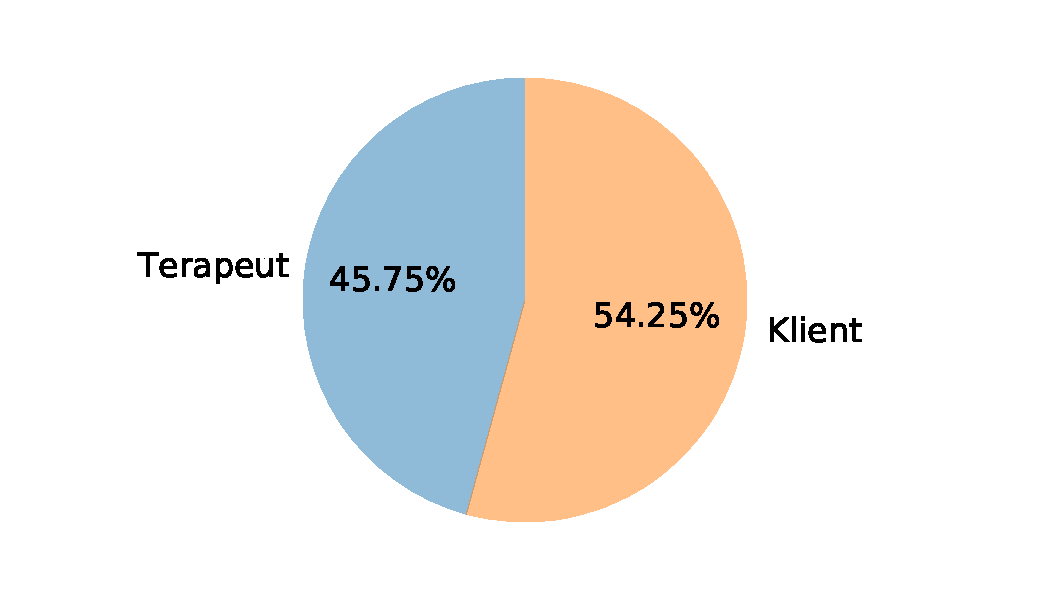
\includegraphics[width=\linewidth]{obrazky-figures/text_plots/speech_ratio.pdf}
    \end{subfigure}%
    \hspace*{\fill}
    \begin{subfigure}{0.5\textwidth}
        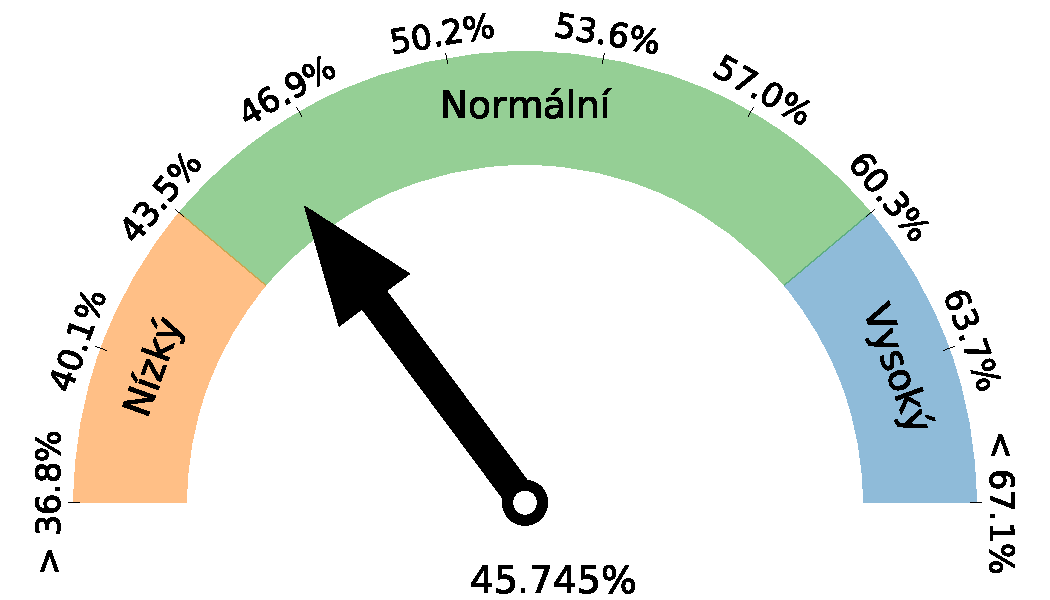
\includegraphics[width=\linewidth]{obrazky-figures/text_plots/speech_ratio_overall.pdf}
    \end{subfigure}
    
    \caption{Poměr doby mluvy mezi terapeutem a klientem. Hodnoty se velmi neliší, oba řečníci mluvili zhruba stejně dlouho. Doba mluvy terapeuta odpovídá dlouhodobému průměru a je k~němu přirovnána na obrázku vpravo.}
    \label{fig:Statisctics_ratio}
\end{figure}


%%%%%%%%%%%%%%%%%%%%%%%%%%%%%%

\subsection{Skákání do řeči}
Mezi další charakteristiky rozhovoru patří skákání do řeči. U~malých dětí je tento jev spojen s~hyperaktivitou, ve skupině vícero mluvčích se jedná o~aspekt pohrdání nebo rozčílení se z~řečového projevu druhé osoby. Avšak v~kontextu psychoterapeutických sezení tento pojem nabývá úplně jiných rozměrů. Psychoterapeuti dokážou skoky do řeči kontrolovat průběh terapie a vést ji správným směrem. Nadměrný výskyt skoků do řeči však může vést k~nespokojenosti jednoho z~mluvčích. V~souhrnné zprávě je proto zahrnut histogram~\cite{histograms} skoků do řeči porovnávající konkrétní sezení se statistikami získanými mezi sezeními. Histogram atypického sezení je zobrazen na~\imageref{fig:Statisctics_butt_ins_reactions}{0}.

\begin{figure}[ht]
    \begin{subfigure}{0.5\textwidth}
        \centering
        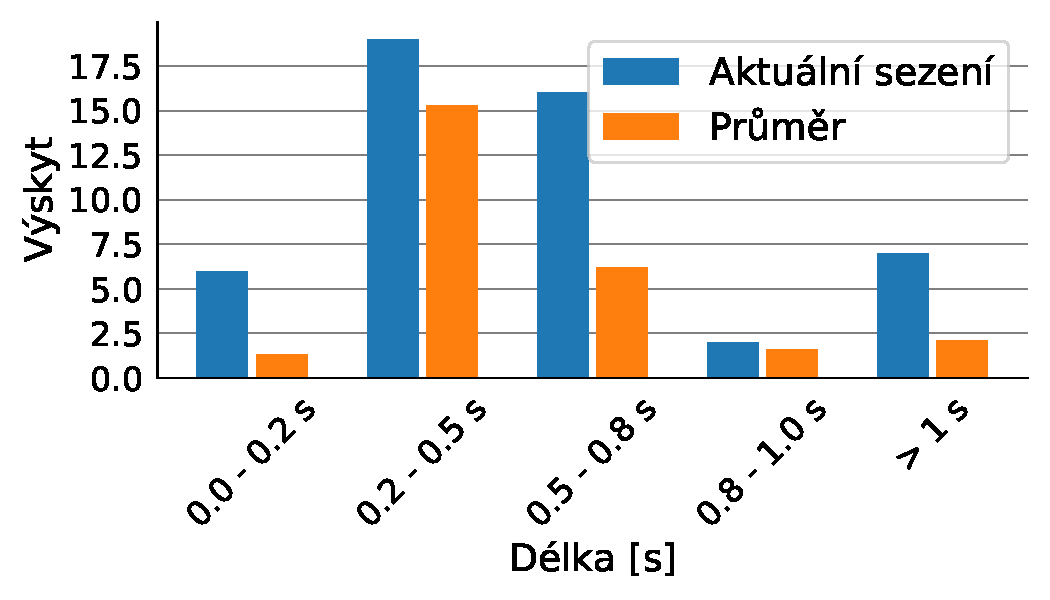
\includegraphics[width=\linewidth]{obrazky-figures/text_plots/client_interruptions.pdf}
        \caption{}
    \end{subfigure}%
    \hspace*{\fill}
    \begin{subfigure}{0.5\textwidth}
        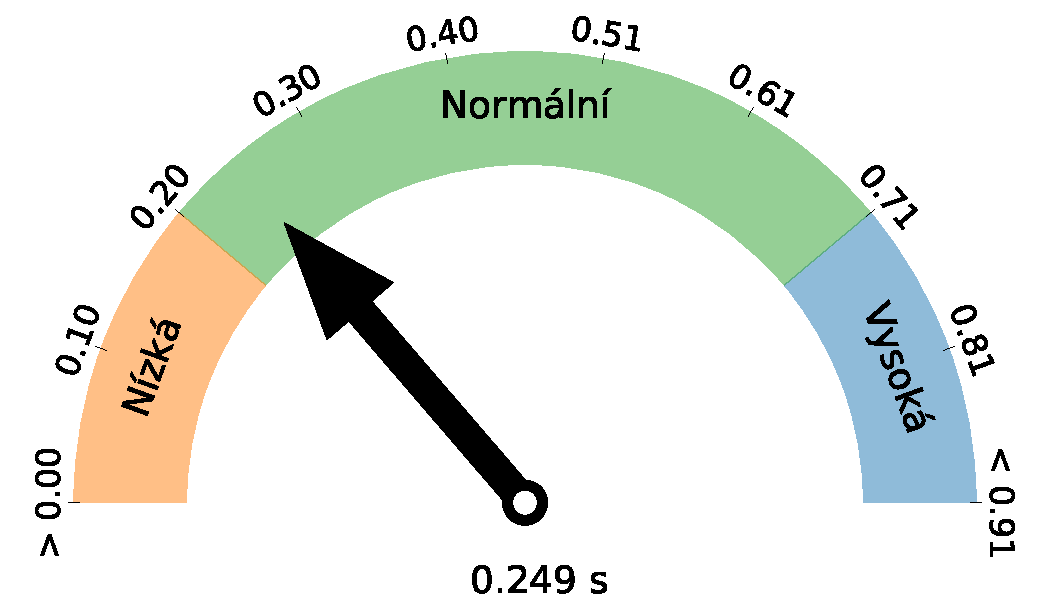
\includegraphics[width=\linewidth]{obrazky-figures/text_plots/reaction_time_therapist.pdf}
        \caption{}
    \end{subfigure}
    \caption{\textbf{(a)} Počty skoků do řeči zobrazené v~podobě histogramu. Hodnoty odpovídají dlouhodobému průměru. \textbf{(b)} Reakční doba je poměrně nízká, blíží se mimo hranici průměrných hodnot.}
    \label{fig:Statisctics_butt_ins_reactions}
\end{figure}

%%%%%%%%%%%%%%%%%%%%%%%%%%%%%%

\subsection{Váhání a délka souvislých úseků řeči}
Pomlky, pauzy v~řeči, zmlknutí a podobné projevy narušují plynulost řeči. Větné pomlky (mezi jednotlivými větami – trvají 0,5 až 1~sekundu) jsou potřebné, řeč se tak nestává lavinou či směsicí slov a je srozumitelná. Pomlky v~jiných místech jsou tzv. „pomlky váhání“. Delší pomlky naznačují, že mluvčí více váhá a není si úplně jist svým sdělením. Mluvčí hovoří nejen tehdy, když mají jasno v~tom, co chtějí sdělit, ale i tehdy, když plánují, o~čem budou v~další fázi hovořit. Běžný posluchač dokáže zaregistrovat náznak zaváhání již při délce pomlky 200~milisekund~\cite{krivohlavy}. Větné pomlky (na rozdíl od pomlk váhání) souvisí i s~pohyby účastníků rozhovoru (např. pokývnutí hlavou, přitakání)~\cite{Dittmann_hesitations}.
Fáze ticha mohou naznačovat nejistotu, rozpaky a váhání, naopak rychlý proud řeči zaujetí a citové vzrušení. Délky souvislých úseků mluvy mohou taktéž ledacos nastínit o~průběhu sezení. Počet váhání a délka souvislých úseků je terapeutovi poskytnuta v~podobě znázorněné na~\imageref{fig:Statisctics_hesitations_speech_len}{}.

\begin{figure}[ht]
    \begin{subfigure}{0.5\textwidth}
        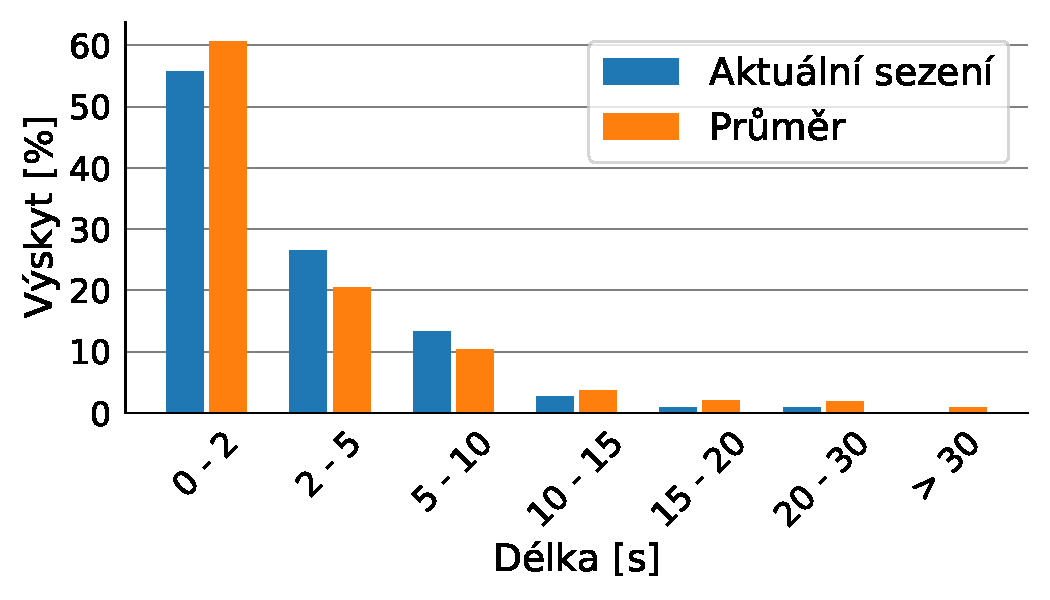
\includegraphics[width=\linewidth]{obrazky-figures/text_plots/bounds_len_client.pdf}
        \caption{}
    \end{subfigure}%
    \hspace*{\fill}
    \begin{subfigure}{0.5\textwidth}
        \centering
        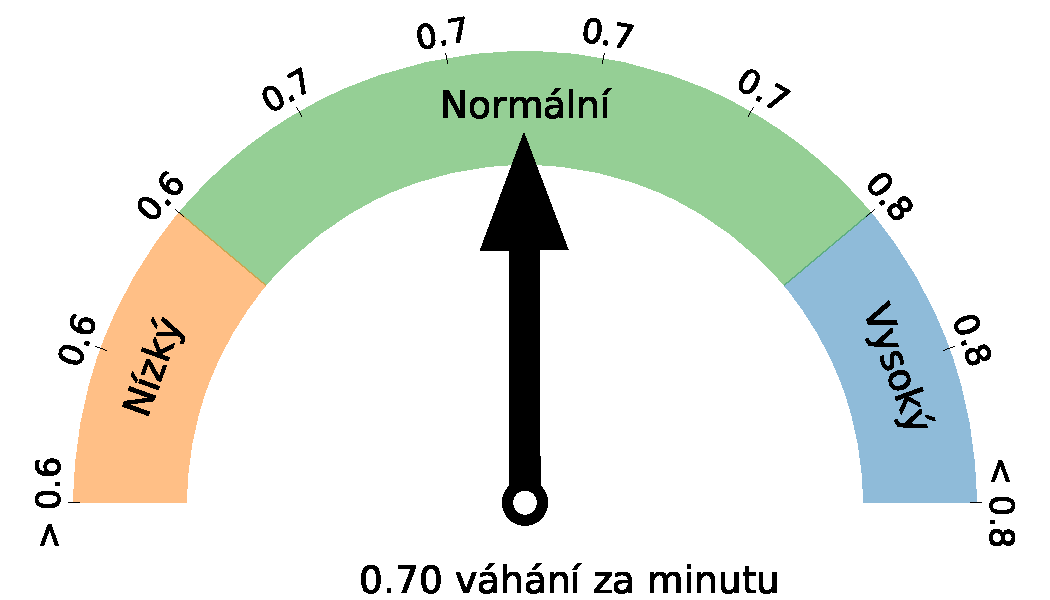
\includegraphics[width=\linewidth]{obrazky-figures/text_plots/hesitations_therapist.pdf}
        \caption{}
    \end{subfigure}
    
     \caption{\textbf{(a)} Délka souvislých úseků řeči. V~nahrávce se nejčastěji objevují krátké věty o~délce 0--2~sekundy. Nebyla detekována žádná věta delší než 30~sekund. \textbf{(b)} Počet váhání za minutu v~mluvě terapeuta. Hodnota 0,7~váhání za minutu přesně odpovídá měřenému průměru. Je však stále poměrně nízká v~porovnání s~průměrem váhání na straně klienta.}
  \label{fig:Statisctics_hesitations_speech_len}
\end{figure}

%%%%%%%%%%%%%%%%%%%%%%%%%%%%%%

\subsection{Reakční doba}
Podobně jako úseky váhání můžeme taktéž klasifikovat podle jejich délky úseky čekání na reakci. Tyto hodnoty se mohou pohybovat od desítek milisekund až po několik sekund. Aby bylo možné tuto hodnotu co nejrychleji interpretovat, je terapeutovi poskytnut graf v~podobě \uv{rychloměru} poskytující porovnání mezi průměrnou hodnotou reakční doby daného sezení a průměrnou hodnotou napříč všemi sezeními v~databázi, případně pouze všemi sezeními daného terapeuta. Tento graf je znázorněný na~\imageref{fig:Statisctics_butt_ins_reactions}{0}. V~ideálním případě by se reakční doby měly pohybovat kolem dlouhodobého průměru, avšak určité druhy terapie, kdy terapeut pokládá složité otázky, vyžadují delší čas na konstrukci odpovědi a dochází tak k~výraznému odklonění od dlouhodobého průměru.

%%%%%%%%%%%%%%%%%%%%%%%%%%%%%%

\subsection{Nejčastěji používané výrazy}
Nejčastěji používané výrazy extrahované z~přepisu nahrávky terapeutovi přinášejí určitý souhrn o~daném sezení. Reprezentace těchto dat v~podobě histogramu nebo v~textové podobě může přinést potřebný náhled do probírané problematiky, avšak technika známá jako \uv{Slovní mrak} (Word Clouds)~\cite{word_cloud} povznáší tento náhled na ještě vyšší úroveň. \imageref{fig:Statisctics_word_cloud}{1} znázorňuje demonstrační mrak získaný z~nahrávky sezení. Terapeut díky tomuto grafu taktéž dokáže zdokonalit svoje vyjadřovací schopnosti omezením nadužívání některých výrazů, které se mohou opakovat v~mracích více sezení.

\begin{figure}[ht]
  \centering
  
\includegraphics[width=\linewidth]{obrazky-figures/text_plots/word_cloud.pdf}
  \caption{Slovní mrak vytvořený z~nahrávky psychoterapeutického sezení. Je možné sledovat, že mluvčí velmi často používal výplňová slova jako např. \uv{vlastně}, \uv{prostě} nebo \uv{jako}.}
  \label{fig:Statisctics_word_cloud}
\end{figure}

%%%%%%%%%%%%%%%%%%%%%%%%%%%%%%
\newpage

\subsection{Mimoslovní složky hlasového projevu}
O~rozpoložení hovořící osoby něco vypovídají i různé těžko popsatelné zvuky při slovním projevu. Mezi nejčastěji používané výplně mluvy patří zvuky jako \uv{ehm ehm...}, \uv{hmmm...}, \uv{éééé...}. Tyto zvuky jsou ve většině případů využívány řečníky pro ujištění posluchačů, že promluva bude pokračovat a nemají ihned reagovat~\cite{krivohlavy}. Tyto mimoslovní složky jsou v~oficiálním přednesu považovány za chyby a mohou být vnímány negativně. Jsou nejčastěji vyvolány vnitřní tísní hovořícího nebo vztahem daným k~osobě naslouchající (před někým se cítíme uvolněně, před jiným napjatě). Snižující se trend výskytu mimoslovních složek hlasového projevu klienta může reprezentovat zvyšující se důvěru mezi klientem a terapeutem, což může vést k~lepším výsledkům terapie. Podobně jako reakční doba je tato hodnota zobrazena pomocí \uv{rychloměru} ukazujícího poměr mezi statistikou aktuálního a ostatních sezení.

%%%%%%%%%%%%%%%%%%%%%%%%%%%%%%

\subsection{Rychlost řeči}
Dalším z~charakteristických ukazatelů je rychlost řeči neboli tempo řeči. Vyjadřuje se nejčastěji počtem vyslovených slabik za určitou časovou jednotku. Pro češtinu se jako průměrné tempo udává hodnota 5 nebo 6 slabik za sekundu, rychlost řeči je však velmi proměnlivá mimo jiné v~závislosti na konkrétním mluvčím, situaci, výstavbě výpovědi, stylu a funkci projevu. Průměrná hodnota charakteristická pro konkrétního člověka se nazývá osobní mluvní tempo. 

Pokud mluvčí zvolí příliš vysoké tempo řeči (např. nad 10 slabik za sekundu), dochází obvykle k~celkové deformaci projevu, protože artikulační orgány nezvládají tak rychle zaujímat patřičné pozice, chybí náležité frázování a odpovídající větná melodie. Posluchač vystavený takovéto překotné mluvě bude mít problémy s~porozuměním. Avšak rovněž přehnaně pomalé tempo (pod dvě slabiky za sekundu) je pro vnímání obtížné. Důležité pro kultivovaný mluvený projev je také umět s~rychlostí řeči funkčně pracovat, tj. nemluvit stále stejně rychle, ale přizpůsobovat tempo řeči jejímu obsahu~\cite{speech_speed}. 

Terapeutovi je představena tato statistika v~podobě liniového grafu obsahující rychlost $N$ stejně dlouhých úseků řeči dané nahrávky. Vektor příslušných hodnot rychlostí úseků $\mathbf{s}$ je vypočten podle následujícího vztahu:

\begin{equation}
    \label{eqn:Speech_speed}
    s_{n} = \frac{1}{N} \sum_{i=1}^{K}\frac{T_{i}^{1}}{T_{i}^{2}}, n \in \{1, \dots, N\},
\end{equation}

kde $\mathbf{T} \in \mathbb{R}^{K \times 2}$ je vektor úseků obsahující pole segmentů řečové aktivity daného úseku $n$ nahrávky obsahující hodnotu počtu slov $T^{1}$ a počtu minut daného segmentu $T^{2}$, $K$ je variabilní velikost pole segmentů daného úseku. Průměrná hodnota rychlosti úseků by měla kolísat mezi 150--200 slovy za minutu~\cite{Rodero_speed}. Demonstrační ukázka je zobrazena na~\imageref{fig:Statisctics_speed}{0}. 

\begin{figure}[ht]
  \centering
  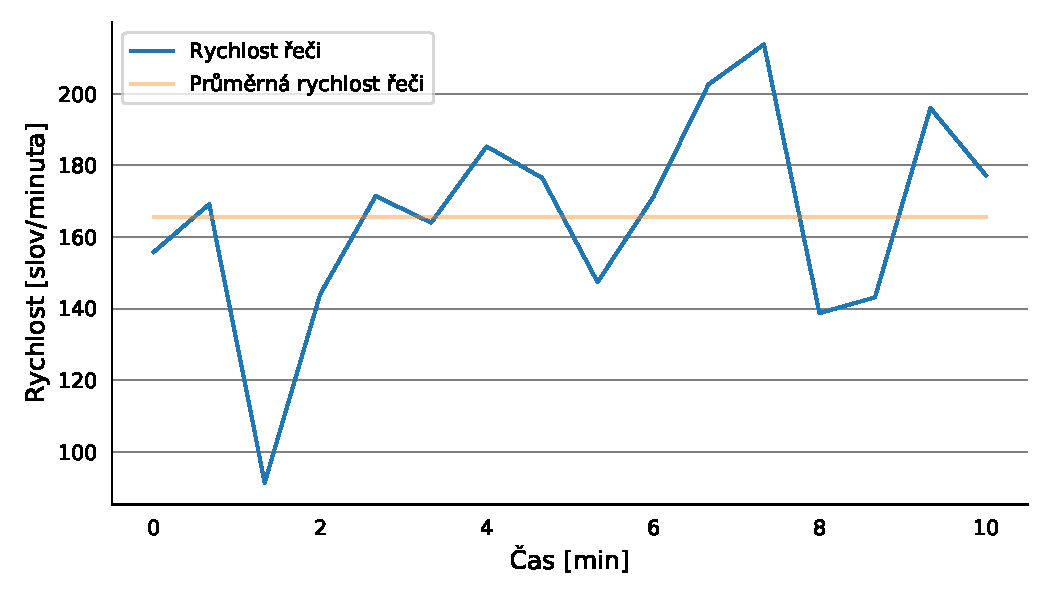
\includegraphics[width=\linewidth]{obrazky-figures/text_plots/speed_therapist.pdf}
  \caption{Měnící se rychlost řeči mluvy terapeuta v~průběhu sezení. Průměrná hodnota leží v~intervalu 150--200 slov za minutu. Vidíme však, že byla detekována výrazná odchylka mezi 1--2 minutou nahrávky. Jelikož se jedná o~začátek sezení, je pravděpodobné, že klient mohl mít problém vysvětlit, co ho trápí a co by chtěl řešit.}
  \label{fig:Statisctics_speed}
\end{figure}

%%%%%%%%%%%%%%%%%%%%%%%%%%%%%%

\subsection{Nálada v~průběhu sezení}
Mezi experimentální statistiky náleží nálada mluvčího v~průběhu sezení. Ta je zkoumaná z~přepisu terapie. Je dostupná pouze pro nahrávky v~anglickém jazyce, jelikož se mi nepodařilo najít hotové řešení pro český jazyk a implementace takového systému by vydala na samostatnou bakalářskou nebo diplomovou práci. Odhad emocí funguje na základě detekce klíčových slov spojených z~různým typem emocí v~textovém přepisu. Tímto způsobem je získán poměr následujících emocí příslušných segmentů textového přepisu:

\begin{itemize}
    \item štěstí,
    \item hněv,
    \item překvapení,
    \item smutek,
    \item strach.
\end{itemize}

Emoce je možné taktéž klasifikovat jako pozitivní a negativní, čímž je terapeutovi poskytnut přehled změn rozpoložení. Jelikož některé segmenty mají délku několika ms, je výstup systému detekce emocí vyhlazen průměrovým filtrem o~velikosti 10 segmentů. Výstup systému pro náladu klienta je znázorněn na~\imageref{fig:Statisctics_mood}{0}.

\begin{figure}[ht]
  \centering
  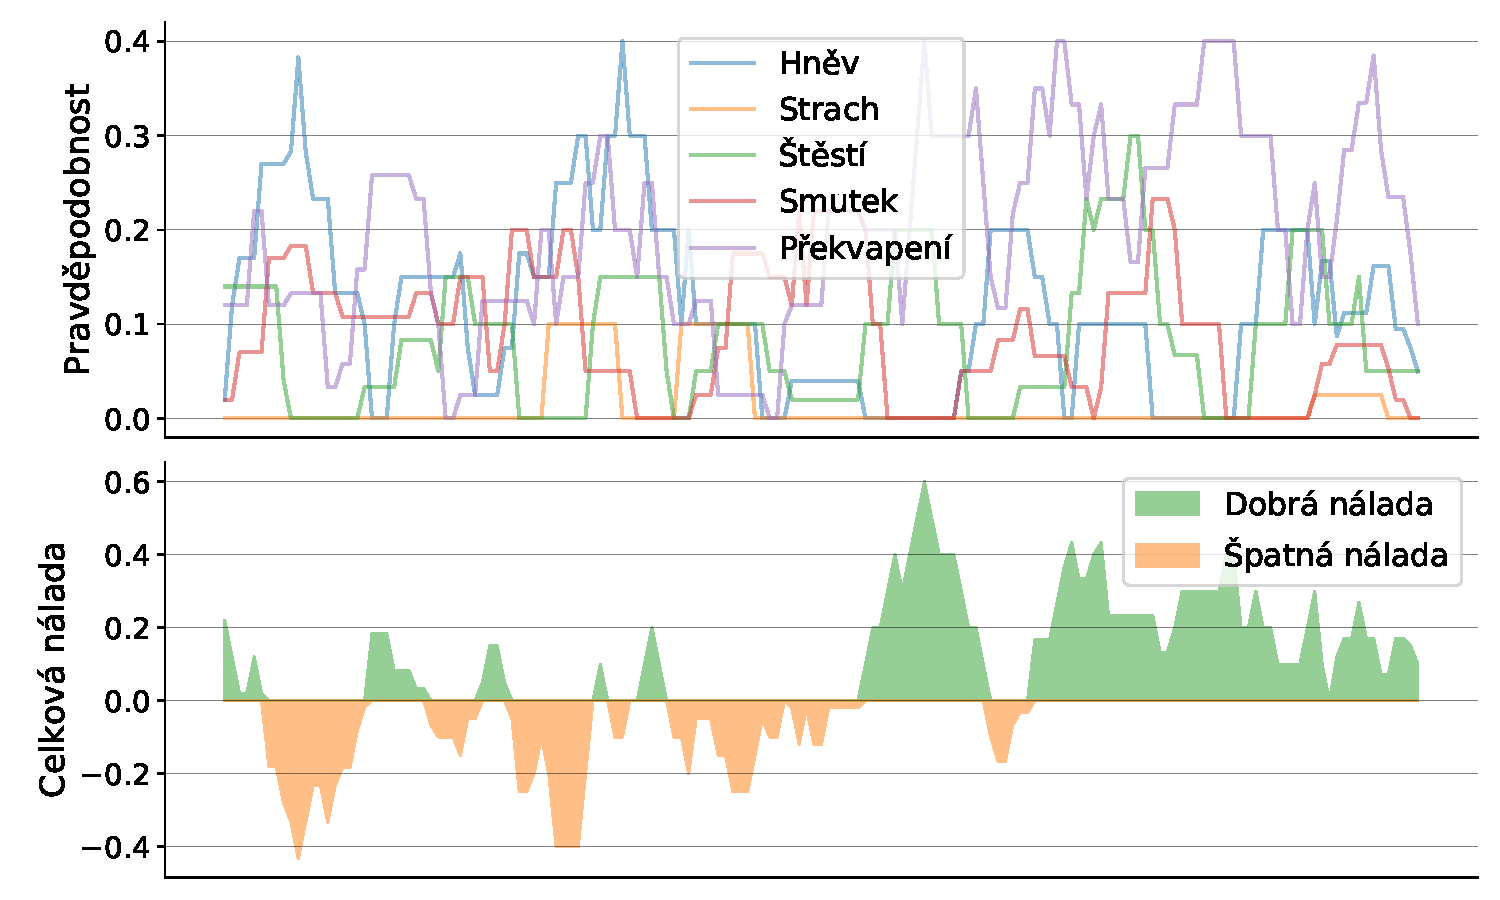
\includegraphics[width=\linewidth]{obrazky-figures/text_plots/client_mood.pdf}
  \caption{Nálada klienta v~průběhu sezení. Jsou zkoumány příslušné emoce a celková nálada. Lze pozorovat kladný trend. Klient z~terapie pravděpodobně odchází s~dobrou náladou.}
  \label{fig:Statisctics_mood}
\end{figure}

%%%%%%%%%%%%%%%%%%%%%%%%%%%%%%

\subsection{Dlouhodobé statistiky}
Aby bylo možné terapeutovi poskytnout informaci o~tom, jak se příslušné sezení liší oproti jiným sezením (sezením terapeuta se stejným klientem, všem sezením daného terapeuta nebo všem dostupným sezením) jsou vypočteny průměrné hodnoty a jejich střední odchylky skupiny zvolených nahrávek. Postupně jsou vypočteny statistiky následujících veličin:

\begin{itemize}
    \item poměr řeči terapeut:klient
    \item reakční doba
    \item počty skoků do řeči a jejich délka
    \item počet váhání za časovou jednotku
    \item procentuální výskyt úseků řeči o~určité délce
    \item počet výplňových slov za minutu
\end{itemize}

Tyto statistiky je následně možné porovnat. Ku příkladu nepřiměřený počet skoků do řeči ze strany terapeuta může naznačovat, že sezení bylo vedeno až příliš konfrontačně.

%%%%%%%%%%%%%%%%%%%%%%%%%%%%%%

\section{Validace výsledků}
\label{section:Validation}
Samotné získání statistik není příliš náchylné na chyby, ale předchází mu proces detekce řečové aktivity, diarizace a rozpoznání řeči, kde chybovost může být velmi vysoká. Z~tohoto důvodu jsou výstupy částí systému validovány vůči referenčním anotacím, aby zvolené řešení bylo co nejúspěšnější. Dataset CallHome obsahuje anotační soubory, vůči kterým je systém možné rovnou validovat. Pro nahrávky projektu DeePsy byly vytvořeny anotace ručně, aby bylo možné ověřit správnou funkcionalitu systému na odlišném typu dat. Byl k~tomu použit volně dostupný nástroj Transcriber\footnote{\url{http://trans.sourceforge.net/en/presentation.php}}.

Nahrávky je možné rozdělit do dvou skupin -- nahrávky s~přeslechem (pořízené prezenčně) a nahrávky pořízené online. V~obou případech jsou k~dispozici skripty zjišťující přesnost použitého systému. Chybovost systému diarizace DER (Diarization error rate) na nahrávkách pořízených prezenčně je definována následovně

\begin{equation}
\label{eqn:DER_offline}
    \text{DER} = \frac{M + F + C}{\text{N}},
\end{equation}

kde $N$ je počet segmentů příslušné nahrávky, $M$ (Miss) označuje počet segmentů, ve kterých alespoň jeden z~mluvčích mluvil, ale systém tento úsek klasifikoval jako neaktivní. $F$ (False alarm) je počet segmentů, ve kterých byla detekována řečová aktivita, ale nikdo v~nahrávce nemluvil, a konečně $C$ (Confusion) je počet segmentů, ve kterých systém zvolil špatného řečníka. Situace, kdy jsou v~referenční anotaci označeni oba mluvčí jako aktivní v~daném úseku a systém detekuje pouze jednoho, není považována za chybu. Jelikož ruční anotace nejsou vždy zcela přesné, evaluační systém dovoluje použití \uv{límce} (collar). \uv{Límec} je úsek referenční anotace, kdy dochází ke změně hodnoty z~ticha na mluvu a opačně. Segmenty nacházející se v~prostoru \uv{límce} nejsou započítány do výsledné chyby diarizace. Standardní velikost \uv{límce} se pohybuje okolo 250 milisekund. \imageref{fig:Collar}{1} ukazuje jakým způsobem probíhá vyhodnocení DER na demonstrační nahrávce.

\begin{figure}[ht]
  \centering
  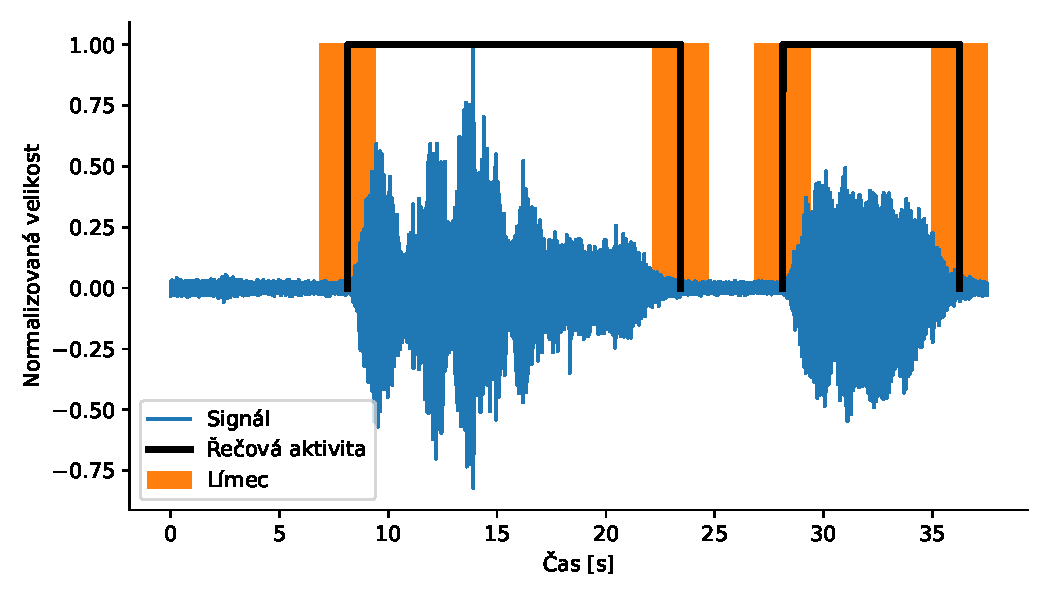
\includegraphics[width=\linewidth]{obrazky-figures/collar.pdf}
  \caption{\uv{Límec} o~velikosti 250 milisekund. Segmenty nacházející se v~oblasti \uv{límce} jsou podbarveny a nejsou vyhodnocovány jako chybné při validaci diarizace.}
  \label{fig:Collar}
\end{figure}


Online nahrávky neobsahují žádný přeslech a mluvčí jsou od sebe odděleni v~příslušných kanálech, což dovoluje definovat chybovost diarizace o~něco striktněji. Chybu diarizace online nahrávky můžeme vypočítat jako průměr chyby detekce řečové aktivity příslušných kanálů nahrávky a definujeme ji jako

\begin{equation}
\label{eqn:DER_online}
    \text{DER} = \frac{M^{1} + F^{1} + M^{2} + F^{2}}{ 2 \cdot N},
\end{equation}
kde $M^{1}$, $M^{2}$, $F^{1}$ a $F^{2}$ označují chyby příslušných kanálů nahrávky. Diarizační chyby komerčně využívaných softwarů nepřekračují hranici 10~\%.

Aby bylo možné porovnat přesnost rozpoznání řeči a tedy jeho strojového přepisu, je chyba takového systému WER (Word error rate) definována jako

\begin{equation}
\label{eqn:WER}
    \text{WER} = \frac{S + I + D}{N},
\end{equation}

kde $S$ (Substitutions) označuje počet záměn slov mezi referenční transkripci a výstupem systému, $I$ (Insertions) počet slov, které jsou ve výstupu systému, ale nevyskytují se v~referenčním výstupu, $D$ (Deletions) počet slov, které jsou v~referenční anotaci, ale nejsou zahrnuty v~přepisu získaném systémem a $N$ počet slov referenčního přepisu. Nevýhodou této metody validace je, že každé slovo má stejnou váhu, což je ale pro účely hrubého odhadu přesnosti systému v~rámci této práce postačující.

%%%%%%%%%%%%%%%%%%%%%%%%%%%%% Implementace %%%%%%%%%%%%%%%%%%%%%%%%%%%%%

\chapter{Implementace}
\label{chap:Implementation}
V~této kapitole jsou představeny nástroje a knihovny použité při implementaci systému pro analýzu rozhovoru dvou osob. Sekce \ref{section:Toolset} zdůvodňuje použití právě jazyka Python\footnote{\url{https://www.python.org/}} a jeho knihoven. V~sekci \ref{section:System} jsou popsány nejdůležitější části systému.  

\section{Použité nastroje}
\label{section:Toolset}
Pro implementaci systému popsaného v~kapitole \ref{chap:System_design} jsem využil skriptovací jazyk Python ve verzi \texttt{3.8.5}. Jazyk Python se v~posledních letech řadí mezi vůbec nejpoužívanější programovací jazyky. S~tím je spojeno množství dostupných knihoven, návodů a dostupných řešení opakujících se problémů. Ačkoliv se jedná o~skriptovací jazyk, Python plně podporuje objektově orientované a procedurální paradigma. Navíc podporuje některé aspekty funkcionálního a aspektově orientované programování. Výše zmíněné výhody a další\footnote{\url{https://medium.com/@mindfiresolutions.usa/python-7-important-reasons-why-you-should-use-python-5801a98a0d0b}} vedou k~tomu, že je programování v~Pythonu velmi komfortní a řešení problémů zabírá zlomek času, jenž by byl nutný k~vyřešení stejného problému v~jiném jazyce. Jistou alternativou pro účely tohoto systému může být implementace v~jazyce Matlab, který je vhodný pro operace nad velkými tenzory. Osobně jsem se ale rozhodl tento jazyk nevyužít a dát přednost Pythonu a knihovnám, které tuto funkcionalitu přinášejí. Python je jazyk interpretovaný a výchozí interpret CPython nemusí být postačující u~výpočetně náročných aplikací. Možnou alternativou je programovací jazyk a překladač Cython, který se snaží dosáhnout vyššího výkonu překladem do nativního kódu a obohacením jazyka o~typový systém.

K~implementaci problémů popsaných v~kapitole \ref{chap:System_design} však využití jazyku Cython nebylo nutné, jelikož existuje knihovna NumPy\footnote{\url{https://numpy.org/}}, která podporuje více dimezionální pole -- tenzory a operace nad nimi. Hodnoty v~polích numpy obsahují datový typ a tím dochází k~značné úspoře alokované paměti a vede to k~vyšší rychlosti operací nad daty a je tak možné se vyvarovat velmi neefektivním smyčkám. Knihovna NumPy obsahuje nespočet matematických či statistických funkcí a operací nad tenzory~\cite{Numpy}. Je základem mnoha dalších knihoven pro analýzu dat -- Pandas\footnote{\url{https://pandas.pydata.org/}}, statistiku -- SciPy\footnote{\url{https://www.scipy.org/}}, strojové učení -- scikit-learn\footnote{\url{https://scikit-learn.org/stable/}}, nebo vizulaizaci -- Matplotlib\footnote{\url{https://matplotlib.org/}}. Je využita v~co nejvyšší míře při operacích nad daty vstupní nahrávky.

Právě knihovna Matplotlib je použita pro vizualizaci všech grafů analýzy sezení. Je to poměrně nízkoúrovňová knihovna, která však s~trochou praxe dovoluje vizualizovat velmi obsáhlé grafy. Opět existuje vysoký počet knihoven, které vycházejí z~Matplotlibu. Za zmínku stojí vysoko-úrovňová vizualizační knihovna seaborn\footnote{\url{https://seaborn.pydata.org/}}, která byla v~rámci vývoje používána, ale v~průběhu byla nahrazena právě knihovnou Matplotlib. Pro účely vizualizace nejpoužívanějších slov je navíc využita knihovna word\_cloud\footnote{\url{https://github.com/amueller/word_cloud}}.

Trénování směsic Gaussovských rozložení usnadňuje již zmíněnaá knihovna scikit-learn a práci s~audio nahrávkami knihovna SciPy.

Při tvorbě výsledné zprávy je využita knihovna Beautiful Soup\footnote{\url{https://www.crummy.com/software/BeautifulSoup/bs4/doc/}}, která dovoluje rychlé a jednoduché parsování dokumentů rodiny XML.

Pro účely získání statistik je využita knihovna pro rozpoznání řeči SpeechRecognition\footnote{\url{https://github.com/Uberi/speech_recognition}} a knihovna pro detekci emocí text2emotion\footnote{\url{https://github.com/aman2656/text2emotion-library}}.

Postup při zpracování nahrávek je uživateli znázorněn pomocí knihovny progress\footnote{\url{https://github.com/verigak/progress/}}.

Rovněž jsou využity standardní knihovny jazyka Python jako re, json, pickle, os nebo argparse. Hojně využívány jsou   f-řetězce~\cite{python_f_string}, které jsou dostupné v~jazyce Python od verze 3.6 a generátorová notace polí~\cite{python_list_comprehension}, která dovoluje vytváření polí bez nutnosti pracného \uv{appendování}.


\section{Systém pro analýzu nahrávek}
\label{section:System}
Navržený systém pro analýzu nahrávek sezení se skládá ze skupiny skriptů. V~kořenové složce \textbf{src} se nacházejí spustitelné skripty odpovídající funkcionalitě bloků popsaných v~kapitole \ref{chap:System_design}. Bloky postupně načítají vstupní soubory, provádějí výpočty a ukládají výstupy, případně tisknou textové řetězce na standardní výstup. Následující pseudokód demonstruje standardní průchod vstupních dat jedním z~bloků.

\begin{minted}{python}
# Importování potřebných knihoven
import libs

# Načtení vstupních argumentů skriptu a jejich validace
args = load_arguments()
# Vytvoření výstupní stromové struktury
check_destination_directory_existence(args.dest)
# Načtení zdrojových souborů
source_files = load_files(args.src, args.extension)

# Postupné zpracování vstupních souborů
for file in source_files:
    # Výpočet výstupních hodnot
    output = process_file(file)
    # Tisk dodatečných informací na standardní výstup
    print(output.text)
    # Uložení výstupních informací
    save_outputs(args.dest, file, output.data)

# Případný tisk stastik o~běhu skriptu a ukončení
print('Additional info')
\end{minted}

Příslušné skripty čerpají z~funkcí, které jsou dostupné v~externích souborech. Ty jsou podle funkcionality rozděleny do příslušných složek. Následující blok demonstruje průběh diarizace nahrávky.

\begin{minted}{python}
...
# Načtení vstupní nahrávky
wav_file, sampling_rate = read_wav_file(join(args.src, file))

# Preemfáze a segmentace pomocí Hammingova okna
signal = process_pre_emphasis(wav_file, params.pre_emphasis_coefficient)
segmented_tracks = process_hamming(signal, sampling_rate,
        params.window_size, params.window_overlap)

# Kalkulace energie segmentů                                   
energy = calculate_energy(segmented_tracks)

# Extrakce Mel-frekvenčních koeficientů
_, mfcc, _ = calculate_mfcc(segmented_tracks, sampling_rate,
        params.cepstral_coef_count)

# Detekce řečové aktivity
vad = energy_gmm_based_vad_propagation(calculate_energy)

# Diarize pomocí směsice Gaussovských rozložení
diarization = gmm_mfcc_diarization(mfcc, vad, calculate_energy)
...
\end{minted}
Systém obsahuje více funkcí, pomocí kterých je možné provést diarizaci. Ve většině případů funkce sdílejí vstupní a výstupní parametry, aby byla záměna co nejjednodušší.

Z~řečově aktivních úseků je vytvořen přepis a poté jsou extrahovány všechny sledované statistiky blíže popsané v~kapitole \ref{chap:FeatureExctraction}. Cílová tvorba souhrnné zprávy, ke které celý proces zpracování nahrávek spěje, probíhá následujícím způsobem.

\begin{minted}{python}
...
for file in files:
    # Načtení přepisu a html šablony
    texts = load_texts(args.text)
    html = load_template(args.template)
    
    # Načtení statistik konkrétního a skupiny sezení
    stats = load_stats(file)
    stats_overall = load_stats_overall(args.stats)
    
    # Nahrazení textací a příloh cílového dokumentu
    add_texts(html, stats, stats_overall, texts, file)
    add_attachments(html, file)
    
    # Tvorba tabulek a grafů
    add_volume_table(html, stats)
    add_plots(html, stats, stats_overall, file)
    
    # Uložení editovaného html kódu do příslušného souboru 
    with open(f'{join(args.path, file)}.html', 'w') as output:
        output.write(str(html))
...
\end{minted}

\subsubsection{Zajímavé úseky kódu}
Jelikož zpracování poměrně dlouhých nahrávek je výpočetně náročné, byl pro účely testování rychlosti kódu implementován dekorátor~\cite{python_decorator} \textbf{@timeit}. Ten získává statistiky o~volání příslušné funkce, což výrazně pomohlo při profilování kódu a vedlo k~jeho následným optimalizacím.

\begin{minted}{python}
import functools
import time

def timeit(func):
    """Dekorátor sloužící k~výpočtu doby běhu funkce"""
    
    # Tvorba nového dekorátu obalujícího funkci
    @functools.wraps(func)
    def new_func(*args, **kwargs):
        # Detekce času volání funkce
        start_time = time.time()
        # Provedení těla funkce
        ret_val = func(*args, **kwargs)
        # Délka běhu = konec -  start
        elapsed_time = time.time() - start_time
        # Tisk časových údajů na standardní výstup
        print(f'function [{func.__name__}] '
              f'finished in {int(elapsed_time * 1000)} ms')
        # Vrácení výsledků funkce
        return ret_val
        
return new_func

# Použití dekorátoru pro kalkulaci délky běhu funkce sum()
@timeit
def sum(a,b):
    return a + b
\end{minted}

Většina kódu pracuje s~daty reprezentovanými v~podobě N-dimenzionálních polí (tenzorů) vytvořených v~knihovně NumPy. Operace nad těmito poli a obecně vektorový přístup může být na první pohled nejasný a bylo nutné detailně prostudovat tuto problematiku. Knihovna NumPy má však skvělou dokumentaci a je tak možné ihned dohledat manuál příslušné funkce/operace. Následující kód demonstruje výpočet procentuálního výskytu úseků mluvy o~příslušné délce pomocí knihovny NumPy.

\begin{minted}{python}
def calculate_segments_len_distribution(bounds):
    """Výpočet histogramu délky úseků mluvy. 
    Vstupem jsou hranice úseků v~podobě dvou dimenzionálního NumPy pole.
    bounds = [[0,10],[12,15]] 
    označuje 2 úseky řeči mající délku 10 a 3 segmenty"""
    
    # Výpočet délky intervalů
    speech_bounds_len = (bounds[:, 1] - bounds[:, 0])

    # Inicializace intervalů distribuce
    bins = np.array([0, 2, 5, 10, 15, 20, 30, np.iinfo(np.int16).max])

    # Získání počtu úseků náležejících příslušným intervalům
    current_counts, _ = np.histogram(speech_bounds_len, bins=bins)
    
    # Normalizace hodnot do rozsahu 0 - 100 % 
    current_counts = (current_counts / np.sum(current_counts)) * 100
    
    return current_counts
\end{minted}

Další poměrně zajímavou pasáží je metoda \textbf{update\_centers} třídy \textit{MyGmm}, která dědí chování z~třídy \textit{GaussianMixture} knihovny scikit-learn. Tato metoda implementuje aktualizaci středních hodnot směsice Gaussovských rozložení o~X \% vzhledem k~novým středům. Kód je podrobněji vysvětlen v~části \textbf{Mel-frekvenční diarizace s~využitím jednoho kanálu} sekce \ref{subsection:Diar_design}. Pro plné pochopení kódu je vhodné taktéž nahlédnout do sekce \ref{subsection:GMM}.

\begin{minted}{python}
import numpy as np
from sklearn.mixture import GaussianMixture
from scipy.special import logsumexp


# Nová třída dědící z~třídy GaussianMixture
class MyGmm(GaussianMixture):

    def update_centers(self, data, shift):
        """Metoda pro aktualizaci středních hodnot GMM směrem 
        k~novým středním hodnotám vypočtených ze vstupní proměnné data. 
        Parametr shift určuje koeficient posunu k~novým středům."""

        # Kalkulace věrohodnosti příslušných vzorků dat 
        weighted_log_gamma = self._estimate_weighted_log_prob(data)
        log_evidence = logsumexp(weighted_log_gamma, axis=1)
        gamma = np.exp(weighted_log_gamma - log_evidence[:, np.newaxis])
        gamma_sum = gamma.sum(axis=0) + \ 
                10  * np.finfo(weighted_log_gamma.dtype).eps

        # Výpočet nových středních hodnot a jejich vah
        new_centers = np.dot(gamma.T, data)
        new_centers_normalized = new_centers / gamma_sum[:, np.newaxis]
        new_weights = gamma_sum / len(data)

        # Aktualizace středních hodnot modelu
        shift_center = shift * new_weights
        shift_center = shift_center[:, np.newaxis]
        self.means_ *= (1 - shift_center)
        self.means_ += shift_center * new_centers_normalized
\end{minted}

%%%%%%%%%%%%%%%%%%%%%%%%%%%%% Experimenty %%%%%%%%%%%%%%%%%%%%%%%%%%%%%

\chapter{Experimenty}
\label{chap:Evaluation}
Detekce řečové aktivity, diarizace a automatické rozpoznání řeči jsou oblasti, ve kterých se mohou lišit i výstupy různých osob provádějící přepis nahrávek. Odhadnout, co přesně která osoba v~daný moment říká, je velmi náročný úkol. Z~tohoto důvodu je vcelku nemožné navrhnout systém, který by dosahoval přesnosti 100 \%. V~této kapitole jsou porovnány metody pro detekci řečové aktivity popsané v~sekci \ref{section:VAD}, diarizační metody navržené v~podsekci \ref{subsection:Diar_design} a dostupné modely tvořící přepis představené v~sekci \ref{section:ASR}.

Pro experimenty nad navrženými metodami byla dostupná data (dataset CallHome a data projektu DeePsy) rozdělena do tří skupin podle charakteru jejích původu. Metody byly postupně vyhodnoceny nad skupinou online, telefonních a prezenčních nahrávek pořízených diktafonem ZOOM H2n. Dataset Callhome obsahuje anotace, vůči kterým je možné validovat. Pro data projektu DeePsy bylo nutné vytvořit referenční anotace. Anotace online nahrávek byly vytvořené ASR systémem pro český jazyk skupiny Speech@fit, přesnost tohoto systému je velmi vysoká a tento výstup je možné považovat za referenční. Pro nahrávky pořízené diktafonem byly referenční anotace vytvořené manuálně pomocí nástroje Transcriber\footnote{\url{http://trans.sourceforge.net/en/presentation.php}}.

\section{Detekce řečové aktivity}
\label{section:VAD_testing}
Detekce řečové aktivity je první a nejdůležitější částí navrženého systému. Provádět rozpoznávání řeči nad segmenty obsahujícími ticho je nežádoucí. Tento požadavek vede k~nutnosti dosáhnout co nejvyšší přesnosti detekce. Implementované metody jsou v~různých konfiguracích spuštěny nad dostupnými nahrávkami a je vyhodnocen počet falešných poplachů -- \uv{False alarm} (segment obsahující ticho klasifikován jako řeč) $F$ a segmentů obsahující řeč klasifikovaných jako ticho $M$ -- \uv{Miss}. 

Testování proběhlo s~různými hodnotami parametrů a s~použitím různých algoritmů pro vyhlazení výstupu. Následující tabulky ukazují hodnoty přesnosti příslušných běhů. Metody, jejichž výstup se může lišit podle pseudonáhodnosti inicializace počátečního stavu, jsou vyhodnoceny ve více iteracích. Přesnost systému $U$ je vypočtena jako

\begin{equation}
    \label{eqn:VAD_Accuracy}
    U = 1 - \frac{F + M}{N},
\end{equation}
kde $N$ je počet segmentů příslušné nahrávky. Pro nahrávky, ve kterých jsou mluvčí odděleni, je celková přesnost počítána jako průměr přesností kanálů. V~případě nahrávek pořízených diktafonem je přesnost počítána pro oba kanály zároveň tak, že dojde k~logické disjunkci řečové aktivity příslušných kanálů.

V~následujících tabulkách se objevují metody, které byly použity pro vyhlazení. Negací úseků se rozumí změna z~řeči na ticho a opačně na úsecích o~délce menší než $X$, které jsou zároveň obklopeny úseky odlišné hodnoty. $p_{loop}$ označuje pravděpodobnost přetrvání v~aktuálním stavu HMM při použití forward-backward algoritmu. Pro všechny níže použité metody je vypočtena střední kvadratická energie $E$, která je následně zobrazena do rozsahu $E \in \langle0;1\rangle$.

\subsubsection{Konstantní práh}
\begin{adjustbox}{width=\textwidth}
\begin{tabular}{ |c|c|c|c|c| } 
    \hline
    \textbf{Práh} & \textbf{Vyhlazení} & \textbf{Miss [\%]} & \textbf{False alarm [\%]} & \textbf{Přesnost [\%]}\\
    \hline
    \multicolumn{5}{|c|}{\multirow{2}{*}{\textbf{CallHome}}} \\
    \multicolumn{5}{|c|}{}\\    
    \hline
    Dynamicky vypočtený  & - & 23,973 & 2,639 & 73,388\\
    \hline
    0,05 & - & 27,746 & 0,226 & 72,028   \\
    \hline
    0,005 & - & 7,768 & 3,960 & 88,272 \\
    \hline
    0,004 & - & 6,766 & 4,856 & 88,378 \\
    \hline
    0,004 & Mediánový filtr (100~ms)  & 5,036 & 4,859 & 90,105 \\
    \hline
    0,004 & Mediánový filtr (300~ms) & 3,881 & 4,601 & 91,518 \\
    \hline
    0,004 &  \begin{tabular}[c]{@{}c@{}}Mediánový filtr (300~ms)\\Negace úseků o~délce $L < 250~\text{ms}$ \end{tabular}  & 3,691 & 4,552 & 91,757 \\
    \hline
    0,006 &  \begin{tabular}[c]{@{}c@{}c@{}}Mediánový filtr (300~ms)\\Negace úseků ticha o~délce $L < 250~\text{ms}$\\Negace úseků řeči o~délce $L < 100~\text{ms}$\end{tabular}  & 4,628 & 3,043 & 92,329 \\
    \hline
    \multicolumn{5}{|c|}{\multirow{2}{*}{\textbf{Online nahrávky}}} \\
    \multicolumn{5}{|c|}{}\\    
    \hline
    0,004 & - & 5,037 & 5,481 & 89,483 \\
    \hline
    0,004 & Mediánový filtr (300~ms) & 3,127 & 5,272 & 91,601 \\
    \hline
    0,006 &  \begin{tabular}[c]{@{}c@{}c@{}}Mediánový filtr (300~ms)\\Negace úseků ticha o~délce $L < 250~\text{ms}$\\Negace úseků řeči o~délce $L < 100~\text{ms}$\end{tabular}  & 3,205 & 3,996 & 92,799 \\
    \hline
    \multicolumn{5}{|c|}{\multirow{2}{*}{\textbf{Nahrávky pořízené diktafonem}}} \\
    \multicolumn{5}{|c|}{}\\    
    \hline
    0,004 & - & 3,099 & 7,104 & 89,797 \\
    \hline
    0,004 & Mediánový filtr (300~ms) & 3,052 & 6,854 & 90,095 \\
    \hline
\end{tabular}
\end{adjustbox}
\subsubsection{Adaptivní práh}
\begin{center}
\begin{adjustbox}{width=0.96\linewidth}
\begin{tabular}{ |c|c|c|c|c|c| } 
    \hline
    \begin{tabular}[c]{@{}c@{}}\textbf{Koeficient růstu}\\\textbf{minimální energie}\end{tabular} & $\lambda$ & \textbf{Vyhlazení} & \textbf{Miss [\%]} & \textbf{False alarm [\%]} & \textbf{Přesnost [\%]}\\
    \hline
    \multicolumn{6}{|c|}{\multirow{2}{*}{\textbf{CallHome}}} \\
    \multicolumn{6}{|c|}{}\\
    \hline
    1,0001 & 0,95 & - & 22,815 & 0,755 & 76,430\\
    \hline
    1,0001 & 0,99 & - & 9,948 & 3,101 & 86,950\\
    \hline
    1,000001 & 0,99 & - & 9,326 & 3,546 & 87,128\\
    \hline
    1,000001 & 0,99 & Mediánový filtr (100~ms) &  7,284 & 3,476 & 89,240\\
    \hline
    1,000001 & 0,99 & Mediánový filtr (300~ms) &  5,589 & 3,290 & 91,120\\
    \hline
    1,000001 & 0,99 & \begin{tabular}[c]{@{}c@{}c@{}}Mediánový filtr (300~ms)\\Negace úseků ticha o~délce $L < 400~\text{ms}$\\Negace úseků řeči o~délce $L < 100~\text{ms}$\end{tabular} & 5,680 & 2,566 & 91,754\\
    \hline
    \multicolumn{6}{|c|}{\multirow{2}{*}{\textbf{Online nahrávky}}} \\
    \multicolumn{6}{|c|}{}\\
    \hline
    1,000001 & 0,99 & - & 7,766 & 3,123 & 89,111\\
    \hline
    1,000001 & 0,99 & Mediánový filtr (300~ms) & 5,169 & 2,918 & 91,914\\
    \hline
    1,000001 & 0,99 & \begin{tabular}[c]{@{}c@{}c@{}}Mediánový filtr (300~ms)\\Negace úseků ticha o~délce $L < 400~\text{ms}$\\Negace úseků řeči o~délce $L < 100~\text{ms}$\end{tabular} & 4,309 & 2,975 & 92,716\\
    \hline
    \multicolumn{6}{|c|}{\multirow{2}{*}{\textbf{Nahrávky pořízené diktafonem}}} \\
    \multicolumn{6}{|c|}{}\\
    \hline
    1,000001 & 0,99 & - & 10,062 & 3,428 & 86,510\\
    \hline
    1,000001 & 0,99 & Mediánový filtr (300~ms) & 9,549 & 3,507 & 86,944\\
    \hline
    1,000001 & 0,99 & \begin{tabular}[c]{@{}c@{}c@{}}Mediánový filtr (300~ms)\\Negace úseků ticha o~délce $L < 400~\text{ms}$\\Negace úseků řeči o~délce $L < 100~\text{ms}$\end{tabular} & 8,917 & 3,527 & 87,555\\
    \hline
\end{tabular}
\end{adjustbox}
\end{center}
\subsubsection{Směsice tří Gaussovských rozložení}
\begin{center}
    \begin{adjustbox}{width=0.96\linewidth}
    \begin{tabular}{ |c|c|c|c|c|c| } 
        \hline
        \textbf{Prahována složka} & \textbf{Práh [\%]} & \textbf{Vyhlazení} &  \textbf{Miss [\%]} & \textbf{False alarm [\%]} & \textbf{Přesnost}  \\
        \hline
        \multicolumn{6}{|c|}{\multirow{2}{*}{\textbf{CallHome}}} \\
        \multicolumn{6}{|c|}{}\\
        \hline
        Ticho & 20 & - & 7,862 & 3,445 & 88,693\\
        \hline
        Ticho & 90 & - & 6,282 & 4,444 & 89,275\\
        \hline
        Šum & 5  & - & 13,716 & 5,724 & 80,560\\
        \hline
        Řeč & 1,5 & - & 10,659 & 3,883 & 85,457\\
        \hline
        Řeč & 90 & - & 30,740 & 0,330 & 68,930\\
        \hline
        Řeč & 1 & $p_{loop} = 0,9$ & 14,341 & 4,373 & 81,286\\
        \hline
        Ticho & 95 & $p_{loop} = 0,9$ & 3,299 & 4,989 & 91,712\\
        \hline
        Ticho & 95 & $p_{loop} = 0,95$ & 3,440 & 4,551 & 92,009\\
        \hline
        Ticho & 95 & \begin{tabular}[c]{@{}c@{}}$p_{loop} = 0,95$\\Mediánový filtr (100~ms)\end{tabular}  & 3,043 & 4,750 & 92,207\\
        \hline
        Ticho & 95 & \begin{tabular}[c]{@{}c@{}}$p_{loop} = 0,95$\\Mediánový filtr (500~ms)\end{tabular}  & 2,453 & 3,995 & 93,552\\
        \hline
        Ticho & 95 & \begin{tabular}[c]{@{}c@{}c@{}c@{}}$p_{loop} = 0,95$\\Mediánový filtr (500~ms)\\Negace úseků ticha o~délce $L < 400~\text{ms}$\\Negace úseků řeči o~délce $L < 100~\text{ms}$\end{tabular}  & 2,410 & 4,016 & 93,574\\
        \hline
        \multicolumn{6}{|c|}{\multirow{2}{*}{\textbf{Online nahrávky}}} \\
        \multicolumn{6}{|c|}{}\\
        \hline
        Ticho & 90 & - & 4,789 & 4,273 & 90,937\\
        \hline
        Řeč & 1,5 & - & 8,401 & 7,809 & 83,790\\
        \hline
        Ticho & 95 & $p_{loop} = 0,95$ & 3,329 & 3,293 & 93,378\\
        \hline
        Ticho & 95 & \begin{tabular}[c]{@{}c@{}c@{}c@{}}$p_{loop} = 0,95$\\Mediánový filtr (500~ms)\\Negace úseků ticha o~délce $L < 400~\text{ms}$\\Negace úseků řeči o~délce $L < 100~\text{ms}$\end{tabular}  & 2,145 & 3,190 & 94,665\\
        \hline
        \multicolumn{6}{|c|}{\multirow{2}{*}{\textbf{Nahrávky pořízené diktafonem}}} \\
        \multicolumn{6}{|c|}{}\\
        \hline
        Ticho & 90 & - & 8,351 & 4,349 & 87,300\\
        \hline
        Ticho & 99 & $p_{loop} = 0,9$ & 4,555 & 5,900 & 89,546\\
        \hline
        Ticho & 96 & \begin{tabular}[c]{@{}c@{}c@{}}$p_{loop} = 0,8$\\Negace úseků ticha o~délce $L < 400~\text{ms}$\\Negace úseků řeči o~délce $L < 100~\text{ms}$\end{tabular}  & 2,427 & 7,875 & 89,698\\
        \hline
    \end{tabular}
    \end{adjustbox}
\end{center}


Nejlepší varianty navržených systémů dosahují na datasetu CallHome průměrné přesnosti v~rozmezí 90--95 \%. Této přesnosti dosahují taktéž na nahrávkách online sezení, což odpovídá předpokladu, že přepis vytvořený ASR systémem pro český jazyk skupiny Speech@fit lze předpokládat za referenční. Horší přesnost je detekována na nahrávkách pořízených diktafonem. Systémy založené na energii nedokážou zcela rozlišit okolní šum od mluvy, a proto se na některých nahrávkách vyskytuje poměrně vysoký \uv{False alarm}, který vede k~nižší přesnosti celého systému. U~nahrávek, které neobsahují značný šum okolí, se přesnost pohybuje v~rozmezí 95--100 \%.

Z~použitých systémů nejlepší výsledky detekce řečové aktivity poskytuje systém směsice tří Gaussovských komponent s~\uv{prahováním} ticha a následným vyhlazením s~použitím forward-backward algoritmu, mediánového filtru a negování krátkých úseků řeči/ticha. Systém selhává na nahrávkách obsahujících vysoký výskyt okolních zvuků. Psychoterapeutická sezení však většinou probíhají v~tichých prostorech.

\section{Diarizace}
\label{section:DIAR_testing}
Z~řečově aktivních segmentů je dále možné určit, kdo je původcem mluvy. U~nahrávek, kde jsou mluvčí odděleni kanály, lze za výstup rovnou považovat detekovanou řečovou aktivitu příslušných kanálů. V~případě nahrávek pořízených diktafonem je nutné provést diarizaci jedním z~algoritmů popsaných v~sekci \ref{section:Diarization}. Jelikož referenční anotace nemusí být vždy přesné, jsou systémy vyhodnoceny s~\uv{límcem} o~velikosti 250~ms a bez \uv{límce}. Následující tabulky ukazují úspěšnosti nejlepších variant navržených systémů.

\subsection{Telefonní a online nahrávky}
Pro online nahrávky je evaluační metrika přísnější a není vyhodnocována diarizační chyba (DER) společně pro oba kanály, ale je vyhodnocen pro úspěšnost detekce řečové aktivity pro oba kanály a tato hodnota je průměrována, čímž vzniká o~něco přísnější metrika.

\begin{table}[H]
\begin{adjustbox}{width=\textwidth}
\begin{tabular}{ |c|c|c|c| } 
    \hline
    \textbf{Typ systému} & \textbf{Miss [\%]} & \textbf{False alarm [\%]} & \textbf{Přesnost [\%]} \\
    \hline
    \begin{tabular}[c]{@{}c@{}c@{}c@{}}\texttt{Konstantní práh}, práh = 0,006\\Mediánový filtr (300~ms)\\Negace úseků ticha o~délce $L < 250~\text{ms}$\\Negace úseků řeči o~délce $L < 100~\text{ms}$\end{tabular}  & \begin{tabular}[c]{@{}c@{}}4,628\\3,070\end{tabular} & \begin{tabular}[c]{@{}c@{}}3,043\\2,177\end{tabular} & \begin{tabular}[c]{@{}c@{}}92,329\\94,752\end{tabular} \\
    \hline
    \begin{tabular}[c]{@{}c@{}c@{}c@{}}\texttt{Adaptivní práh}, růst = 1,000001, $\lambda = 0,99$\\Mediánový filtr (300~ms)\\Negace úseků ticha o~délce $L < 400~\text{ms}$\\Negace úseků řeči o~délce $L < 100~\text{ms}$\end{tabular}  & \begin{tabular}[c]{@{}c@{}}5,680\\3,828\end{tabular} & \begin{tabular}[c]{@{}c@{}}2,566\\1,797\end{tabular} & \begin{tabular}[c]{@{}c@{}}91,754\\94,375\end{tabular} \\
    \hline
    \begin{tabular}[c]{@{}c@{}c@{}c@{}c@{}}\texttt{Směsice tří Gaussovských rozložení}\\složka -- ticho, práh = 95\%, $p_{loop} = 0,95$\\Mediánový filtr (500~ms)\\Negace úseků ticha o~délce $L < 400~\text{ms}$\\Negace úseků řeči o~délce $L < 100~\text{ms}$\end{tabular}  & \begin{tabular}[c]{@{}c@{}}2,453\\1,623\end{tabular} & \begin{tabular}[c]{@{}c@{}}3,995\\2,355\end{tabular} & \begin{tabular}[c]{@{}c@{}}93,552\\96,021\end{tabular} \\
    \hline
\end{tabular}
\end{adjustbox}
\caption{\label{tab:Diar_callhome} Úspěšnost diarizace závislá na použité metodě detekce řečové aktivity datasetu CallHome. Příslušné buňky metrik systému obsahují dvě hodnoty. Horní hodnota odpovídá evaluaci bez použití \uv{límce} a dolní evaluaci s~použitím \uv{límce} o~velikosti 250~ms.}
\end{table}

\begin{table}[H]
\begin{adjustbox}{width=\textwidth}
\begin{tabular}{ |c|c|c|c| } 
    \hline
    \textbf{Typ systému} & \textbf{Miss [\%]} & \textbf{False alarm [\%]} &  \textbf{Přesnost [\%]}\\
    \hline
    \begin{tabular}[c]{@{}c@{}c@{}c@{}}\texttt{Konstantní práh}, práh = 0,006\\Mediánový filtr (300~ms)\\Negace úseků ticha o~délce $L < 250~\text{ms}$\\Negace úseků řeči o~délce $L < 100~\text{ms}$\end{tabular} & \begin{tabular}[c]{@{}c@{}}3,205\\1,961\end{tabular} & \begin{tabular}[c]{@{}c@{}}3,996\\3,459\end{tabular} & \begin{tabular}[c]{@{}c@{}}92,799\\94,579\end{tabular} \\
    \hline
    \begin{tabular}[c]{@{}c@{}c@{}c@{}}\texttt{Adaptivní práh}, růst = 1,000001, $\lambda = 0,99$\\Mediánový filtr (300~ms)\\Negace úseků ticha o~délce $L < 400~\text{ms}$\\Negace úseků řeči o~délce $L < 100~\text{ms}$\end{tabular} & \begin{tabular}[c]{@{}c@{}}4,309\\2,860\end{tabular} & \begin{tabular}[c]{@{}c@{}}2,975\\2,589\end{tabular} & \begin{tabular}[c]{@{}c@{}}92,716\\94,551\end{tabular} \\
    \hline
    \begin{tabular}[c]{@{}c@{}c@{}c@{}c@{}}\texttt{Směsice tří Gaussovských rozložení}\\složka -- ticho, práh = 95\%, $p_{loop} = 0,95$\\Mediánový filtr (500~ms)\\Negace úseků ticha o~délce $L < 400~\text{ms}$\\Negace úseků řeči o~délce $L < 100~\text{ms}$\end{tabular} & \begin{tabular}[c]{@{}c@{}}2,145\\1,227\end{tabular} & \begin{tabular}[c]{@{}c@{}}3,190\\2,551\end{tabular} & \begin{tabular}[c]{@{}c@{}}94,665\\96,222\end{tabular} \\
    \hline
\end{tabular}
\end{adjustbox}
\caption{\label{tab:Diar_online_deepsy} Úspěšnost diarizace závislá na použité metodě detekce řečové aktivity nahrávek online psychoterapeutických sezení projektu DeePsy. Obdobně jak v~předchozí tabulce příslušné buňky metrik systému obsahují dvě hodnoty. Horní hodnota odpovídá evaluaci bez použití \uv{límce} a dolní evaluaci s~použitím \uv{límce} o~velikosti 250~ms.}
\end{table}

\subsection{Nahrávky pořízené diktafonem}
S~nahrávkami pořízenými diktafonem ZOOM H2n byly provedeny experimenty pomocí navržených metod. Nahrávky prezenčních psychoterapeutických sezení však byly do systému projektu DeePsy nahrány až v~době odevzdání této práce, a tak nebylo zcela možné vytvořit ruční anotace většího množství těchto nahrávek. Optimální parametry navržených metod tak byly validovány pouze na části dostupných nahrávek, které byly do té doby anotovány. Metody jsou taktéž porovnány se značně robustnějším systémem VBHMM x-vectors Diarization (VBx)~\cite{VBx}, který provádí diarizaci na nahrávce s~jedním kanálem (pro tyto účely jsou kanály vstupních nahrávek spojeny do jednoho kanálu pomocí nástroje SoX\footnote{\url{http://sox.sourceforge.net/sox.html}}). Aby nebyla chyba diarizace DER (definována v~sekci~\ref{section:Validation}) zkreslená chybou způsobenou nepřesnou detekcí řečové aktivity, je načtená její referenční podoba ze souborů s~příponou \texttt{.rttm} a nad ní je provedena diarizace. Tento způsob dovoluje pouze vyhodnocení chyby $C$ (Confusion), kdy systém označí jako původce řeči terapeuta, avšak je jím klient a opačně. Hodnoty $F$ (False alarm) a $M$ (Miss) jsou rovné nule. 

Navržené metody nejsou schopné detekovat více řečníků v~jednom segmentu, jelikož provádějí diarizaci tvrdým rozhodnutím na základě pravděpodobností mluvy jednotlivých řečníků. Toto omezení znemožňuje detekci skoků do řeči, a z~tohoto důvodu nejsou skoky do řeči v~případě prezenčního sezení zahrnuty do souhrnné zprávy. Aby bylo možné tyto statistiky zahrnout, výstupem diarizace by musela být pravděpodobnost mluvy každého z~řečníků a u~segmentů, kde by byla pravděpodobnost podobně veliká, by bylo možné pomocí dalšího modelu detekovat pravděpodobnost, že mluví oba řečníci. 

Následující tabulka obsahuje tuto chybu označenou v~rovnici chybovosti diarizace \ref{eqn:DER_offline} jako $C$ (Confusion). Zároveň je vyhodnoceno $P_{1}$ jako procento počtu segmentů mluvy terapeuta, kdy byl terapeut klasifikován jako klient a $P_{2}$ jako procento počtu segmentů mluvy klienta, kdy byl klient klasifikován jako terapeut. Obdobně jako v~předchozím případě jsou metody vyhodnoceny s~\uv{límcem} o~velikosti 250~ms a bez \uv{límce}.


\begin{table}[H]
\begin{adjustbox}{width=\textwidth}
\begin{tabular}{ |c|c|c|c|c|c| } 
    \hline
    \textbf{Metoda} & \textbf{Vyhlazení} & \textbf{Límec} &  $\mathbf{P}_{1}$ [\%]  & $\mathbf{P}_{2}$ [\%] & \ $\mathbf{C}$ [\%] \\
    \hline
    Energetická diarizace -- $\text{E} \in \langle0;1\rangle$ & - & 0  & 28,953 & 18,435 & 21,997 \\
    \hline
    Energetická diarizace & - & 0 &38,231 & 16,227 & 13,378 \\
    \hline
    Energetická diarizace & Mediánový filtr (300~ms) & 0 & 36,182 &  9,822 & 9,009 \\
    \hline
    Energetická diarizace & Mediánový filtr (300~ms) & 250 & 35,261 &  9,057 & 7,594\\
    \hline
    Energetická diarizace & Mediánový filtr (1~s) & 0 & 36,548 & 9,139 & 8,604 \\
    \hline
    Energetická diarizace & Mediánový filtr (1~s) & 250 & 35,433 & 8,065 & 7,043 \\
    \hline
\end{tabular}
\end{adjustbox}
\caption{\label{tab:Diar_energy_deepsy} Úspěšnost diarizačního systému založeného na rozhodnutí podle vyšší z~energií příslušných segmentů kanálů nahrávky.}
\end{table}

Ačkoliv je chybovost systému energetické diarizace $C$ poměrně nízká, systém naprosto selhává v~případě, kdy energie jednoho z~kanálu je vyšší v~průběhu celého sezení, jak je zobrazeno na~\imageref{fig:Energy_diar_failure}{0}, což odpovídá velmi vysoké hodnotě chyby $P_{1}$.

\begin{figure}[ht]
  \centering
  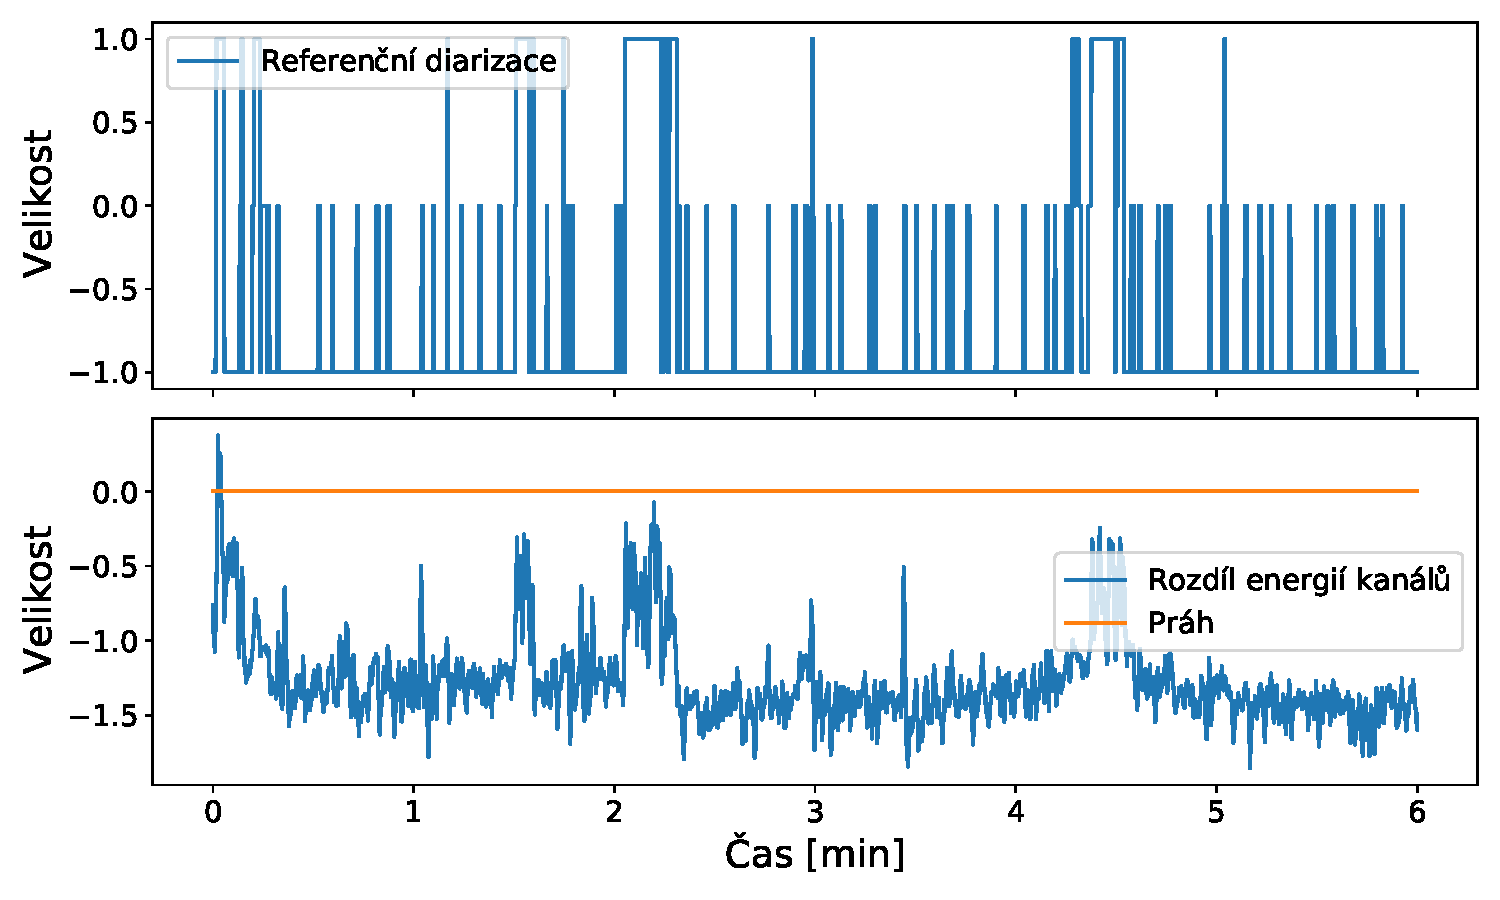
\includegraphics[width=\linewidth]{obrazky-figures/energy_diff.pdf}
  \caption{Na horním obrázku jsou zobrazeny hodnoty referenční diarizace příslušných segmentů. Na dolním obrázku je vidět rozdíl energie kanálu terapeuta oproti energii kanálu klienta, podle kterého následně dochází k~určení řečníka. Hodnota $1$ označuje segmenty, ve kterých hovořil terapeut, $0$ ticho a $-1$ segmenty, ve kterých hovořil klient. Je pravděpodobné, že byla špatně zvolena pozice diktafonu, a tak je energie kanálu klienta po celou dobu vyšší, což vede ke špatné detekci mluvčího. Možným řešením může byt normalizace energie do stejného rozsahu nebo prahování pomocí průměrné hodnoty rozdílu energií, tato řešení však selhávají na ostatních nahrávkách, kde byla správně nastavena poloha diktafonu.}
  \label{fig:Energy_diar_failure}
\end{figure}

Tabulka~\ref{tab:Diar_mfcc1_deepsy} zobrazuje chybovosti metod založených na shlukování segmentů podle mel-frekvenčních koeficientů, které byly navrženy za účelem diarizace nahrávek prezenčních sezení.

\begin{table}[H]
\begin{adjustbox}{width=\textwidth}
\begin{tabular}{ |c|c|c|c|c|c|c| } 
    \hline
    \begin{tabular}[c]{@{}c@{}}\textbf{MFCC}\\\textbf{koeficienty}\end{tabular} & \begin{tabular}[c]{@{}c@{}}\textbf{Adaptace GMM}\\\textbf{podle}\end{tabular}  & \textbf{Vyhlazení} & \textbf{Límec} & $\mathbf{P}_{1}$ [\%]  & $\mathbf{P}_{2}$ [\%] & \ $\mathbf{C}$ [\%]  \\
    \hline
    10 MFCC jednoho kanálu & \begin{tabular}[c]{@{}c@{}}10~\% segmentů $\mathbf{e}_{d}$\\posun $\text{\boldmath$\mu$}$ o~5~\%\end{tabular} & - & 0 & 34,240 & 42,742 & 31,838 \\
    \hline
    20 MFCC jednoho kanálu & \begin{tabular}[c]{@{}c@{}}10~\% segmentů $\mathbf{e}_{d}$\\posun $\text{\boldmath$\mu$}$ o~5~\%\end{tabular} & - & 0 & 33,026 & 42,082 & 31,463 \\
    \hline
    20 MFCC jednoho kanálu & \begin{tabular}[c]{@{}c@{}}10~\% segmentů $\mathbf{e}_{d}$\\posun $\text{\boldmath$\mu$}$ o~5~\%\end{tabular} & $mean(\mathbf{e}_{d}; 0,5~s)$  & 0 & 30,212 & 40,889 & 30,438  \\
    \hline
    20 MFCC jednoho kanálu & \begin{tabular}[c]{@{}c@{}}10~\% segmentů $\mathbf{e}_{d}$\\posun $\text{\boldmath$\mu$}$ o~5~\%\end{tabular} & \begin{tabular}[c]{@{}c@{}}$mean(\mathbf{e}_{d}; 0,5~s)$\\$fb(\mathbf{p}^{1}|\mathbf{p}^{2}; 0,9)$\end{tabular}  & 0 &   14,497 & 32,379 & 21,935  \\
    \hline
    20 MFCC jednoho kanálu & \begin{tabular}[c]{@{}c@{}}10~\% segmentů $\mathbf{e}_{d}$\\posun $\text{\boldmath$\mu$}$ o 5~\%\end{tabular} & \begin{tabular}[c]{@{}c@{}c@{}}$mean(\mathbf{e}_{d}; 0,5~s)$\\$fb(\mathbf{p}^{1}|\mathbf{p}^{2}; 0,9)$\\$mean(\mathbf{r}; 0,5~s)$\end{tabular} & 0 &  12,974 & 25,623 & 17,715 \\
    \hline
\end{tabular}
\end{adjustbox}
\caption{\label{tab:Diar_mfcc1_deepsy} Úspěšnost diarizačního systému založeného na shlukování segmentů podle mel-frekvenčních koeficientů. Notace $\mathbf{p}^{1}|\mathbf{p}^{2}$ označuje konkatenaci dvou vektorů do matice. $fb(\mathbf{v}; x)$ označuje provedení forward-backward algoritmu nad maticí $\mathbf{v}$ s hodnotou $p_{loop} = x$. Obdobně $mean(\mathbf{v}; x)$ reprezentuje aplikaci průměrového filtru nad vektorem $\mathbf{v}$ o velikosti $x$ sekund.}
\end{table}

Je patrné, že takto navržený systém selhává. Důvodem je nejistota systému v~některých segmentech způsobená nízkým rozdílem pravděpodobností vektoru $\mathbf{r}$. \imageref{fig:MFCC_diar_failure}{1} zobrazuje princip fungování navrženého systému a ukazuje, kde systém selhává. 

\begin{figure}[H]
  \centering
  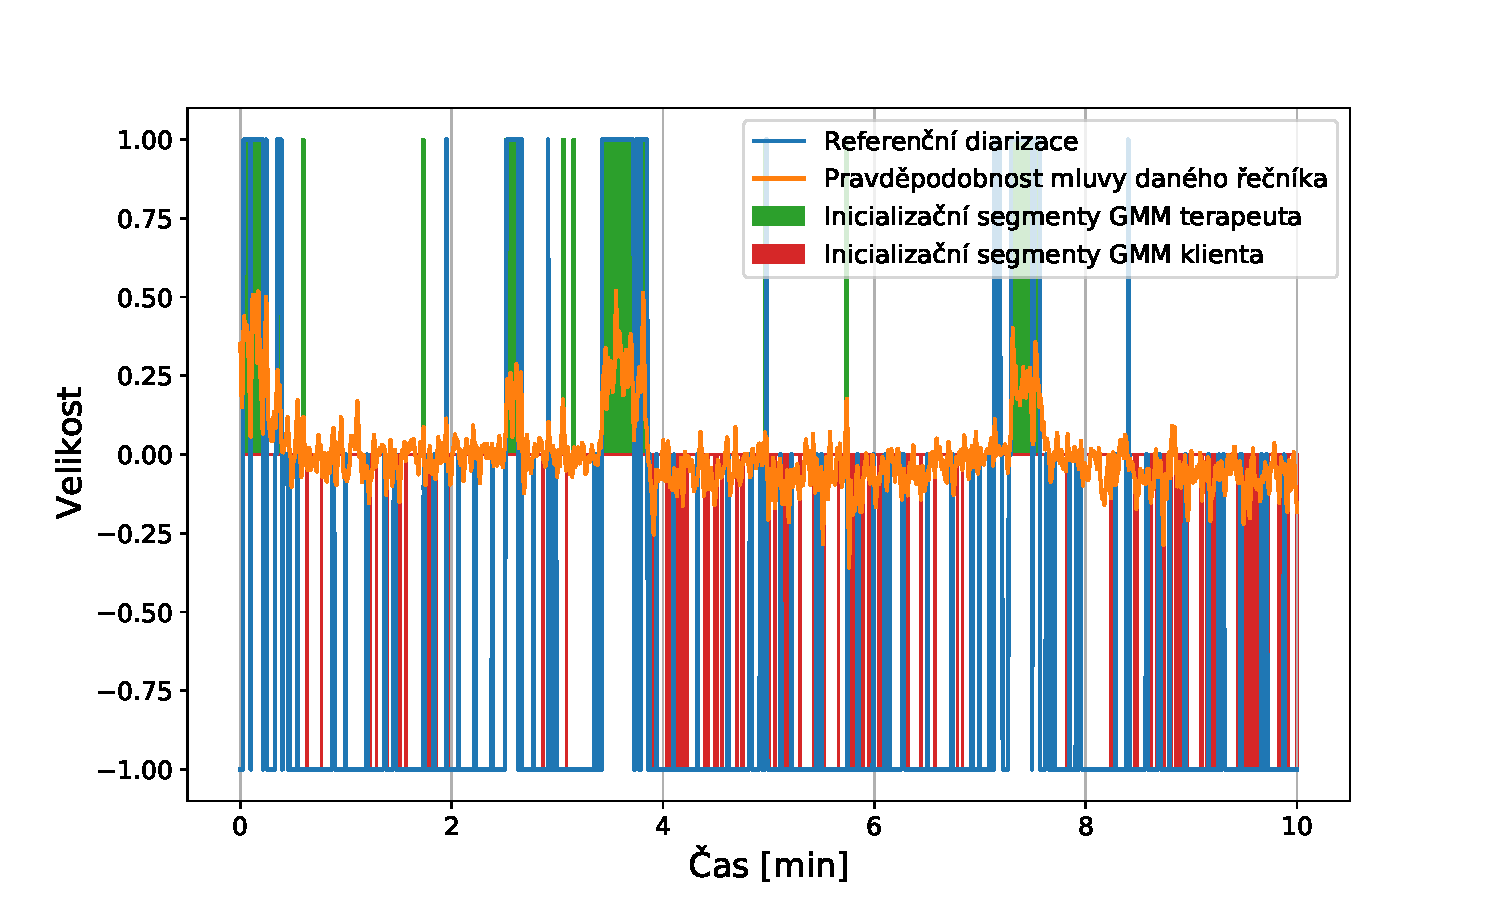
\includegraphics[width=0.97\linewidth]{obrazky-figures/mfcc_diff.pdf}
  \caption{Princip fungování systému diarizace pomocí mel-frekvenčních koeficientů. Hodnota $1$ odpovídá segmentům, ve kterých mluví terapeut a $-1$ segmentům, ve kterých mluví klient. $0$ odpovídá tichu. Oranžová křivka zobrazuje pravděpodobnost mluvy příslušných osob. Je patrné, že systém dokáže velmi dobře detekovat segmenty, pomocí nichž byla provedena adaptace -- tyto segmenty jsou podbarvené zeleně a červeně. V~mnoha segmentech si však systém není jistý a hodnoty kolísají mezi kladnou a zápornou hodnotou na \textit{ose y}, což způsobuje poměrně vysokou chybu diarizace.}
  \label{fig:MFCC_diar_failure}
\end{figure}

Navrženou metodu a její deriváty, jejichž chybovost byla téměř identická, proto bylo nutné podrobit dalšímu zpracování. Je tedy použita metoda prahování příslušných složek. Dokud není překročen příslušný práh, zůstává hovořícím mluvčí předchozího segmentu. Tuto metodu je možné definovat následovně:

\begin{equation}
    d_{n} = \begin{cases}
        2   & r_{n} >= F_{2}\\
        1   & r_{n} <= F_{1}\\
        0   & u_{n}\\
        d_{n - k} & jinak
               \end{cases}, n \in \{ 1, \dots, N\},
\end{equation}
kde $d_{n - k}$ je první aktivní segment, $F_{1}$ je práh vypočtený jako $\frac{\min(\mathbf{r})}{5}$ a $F_{2}$ jako $\frac{\max(\mathbf{r})}{5}$. Zbylé notace hodnot odpovídají těm, které byly zavedeny v~sekci~\ref{subsection:Diar_design}. Tabulka~\ref{tab:Diar_mfcc2_deepsy} ukazuje chybovost upravených metod systému.

\begin{table}[ht]
\centering
\begin{adjustbox}{width=\textwidth}
\begin{tabular}{ |c|c|c|c|c|c|c| } 
    \hline
    \begin{tabular}[c]{@{}c@{}}\textbf{MFCC}\\\textbf{koeficienty}\end{tabular} & \begin{tabular}[c]{@{}c@{}}\textbf{Adaptace GMM}\\\textbf{podle}\end{tabular}  & \textbf{Vyhlazení} & \textbf{Límec} & $\mathbf{P}_{1}$ [\%]  & $\mathbf{P}_{2}$ [\%] & \ $\mathbf{C}$ [\%]  \\
    \hline
    20 MFCC jednoho kanálu & \begin{tabular}[c]{@{}c@{}}10~\% segmentů $\mathbf{e}_{d}$\\posun $\text{\boldmath$\mu$}$ o~5~\%\end{tabular} & \begin{tabular}[c]{@{}c@{}c@{}}$mean(\mathbf{e}_{d}; 0,5~s)$\\$fb(\mathbf{p}^{1}|\mathbf{p}^{2}; 0,9)$\\$mean(\mathbf{r}; 0,5~s)$\end{tabular} & 0 & 8,753 & 14,873 & 10,262 \\
    \hline
    \begin{tabular}[c]{@{}c@{}c@{}}20 MFCC jednoho kanálu +\\20 delta koeficientů \end{tabular} & \begin{tabular}[c]{@{}c@{}}10~\% segmentů $\mathbf{e}_{d}$\\posun $\text{\boldmath$\mu$}$ o~5~\%\end{tabular} & \begin{tabular}[c]{@{}c@{}c@{}}$mean(\mathbf{e}_{d}; 0,5~s)$\\$fb(\mathbf{p}^{1}|\mathbf{p}^{2}; 0,9)$\\$mean(\mathbf{r}; 0,5~s)$\end{tabular} & 250 & 5,047 & 11,617 & 7,779 \\
    \hline
    \begin{tabular}[c]{@{}c@{}c@{}}20 MFCC jednoho kanálu +\\20 delta koeficientů \end{tabular} & \begin{tabular}[c]{@{}c@{}}10~\% segmentů $\mathbf{e}_{d}$\\posun $\text{\boldmath$\mu$}$ o~5~\%\end{tabular} & \begin{tabular}[c]{@{}c@{}c@{}}$mean(\mathbf{e}_{d}; 0,5~s)$\\$fb(\mathbf{p}^{1}|\mathbf{p}^{2}; 0,9)$\\$mean(\mathbf{r}; 0,5~s)$\end{tabular} & 250 & 3,434 & 10,071 & 6,043 \\
    \hline
    \begin{tabular}[c]{@{}c@{}c@{}}(20 + 20) MFCC kanálů +\\(20 + 20) delta koeficientů \end{tabular} & \begin{tabular}[c]{@{}c@{}}10~\% segmentů $\mathbf{e}_{d}$\\posun $\text{\boldmath$\mu$}$ o~5~\%\end{tabular} & \begin{tabular}[c]{@{}c@{}c@{}}$mean(\mathbf{e}_{d}; 0,5~s)$\\$fb(\mathbf{p}^{1}|\mathbf{p}^{2}; 0,9)$\\$mean(\mathbf{r}; 0,5~s)$\end{tabular} & 0 & 5,144 & 10,933 & 6,629 \\
    \hline
    \begin{tabular}[c]{@{}c@{}c@{}}(20 + 20) MFCC kanálů +\\(20 + 20) delta koeficientů \end{tabular} & \begin{tabular}[c]{@{}c@{}}10~\% segmentů $\mathbf{e}_{d}$\\posun $\text{\boldmath$\mu$}$ o~5~\%\end{tabular} & \begin{tabular}[c]{@{}c@{}c@{}}$mean(\mathbf{e}_{d}; 0,5~s)$\\$fb(\mathbf{p}^{1}|\mathbf{p}^{2}; 0,9)$\\$mean(\mathbf{r}; 0,5~s)$\end{tabular} & 250 & 1,936 & 9,855 & 5,519 \\
    \hline
    \begin{tabular}[c]{@{}c@{}c@{}}(20 + 20) MFCC kanálů +\\(20 + 20) delta koeficientů\\\end{tabular} & \begin{tabular}[c]{@{}c@{}c@{}}10~\% segmentů $\mathbf{e}_{d}$\\posun $\text{\boldmath$\mu$}$ o~5~\%\\2 iterace adaptace\end{tabular} & \begin{tabular}[c]{@{}c@{}c@{}}$mean(\mathbf{e}_{d}; 0,5~s)$\\$fb(\mathbf{p}^{1}|\mathbf{p}^{2}; 0,9)$\\$mean(\mathbf{r}; 0,5~s)$\end{tabular} & 0 & 5,990 & 14,652 & 9,420 \\
    \hline
    \begin{tabular}[c]{@{}c@{}c@{}}(20 + 20) MFCC kanálů +\\(20 + 20) delta koeficientů\\\end{tabular} & \begin{tabular}[c]{@{}c@{}c@{}}10~\% segmentů $\mathbf{e}_{d}$\\posun $\text{\boldmath$\mu$}$ o~5~\%\\2 iterace adaptace\end{tabular} & \begin{tabular}[c]{@{}c@{}c@{}}$mean(\mathbf{e}_{d}; 0,5~s)$\\$fb(\mathbf{p}^{1}|\mathbf{p}^{2}; 0,9)$\\$mean(\mathbf{r}; 0,5~s)$\end{tabular} & 250 & 4,398 & 13,413 & 7,611 \\
    \hline
\end{tabular}
\end{adjustbox}
\caption{\label{tab:Diar_mfcc2_deepsy} Chybovost metod po aplikaci prahování. Nejlepší výsledky jsou dosaženy pomocí metody používající mel-frekvenční koeficienty obou kanálu bez následné adaptace v~druhé iteraci.}
\end{table}

Nejlépe fungující metoda byla dále podrobena sérii dalších pokusů, jejichž výsledky ilustruje tabulka~\ref{tab:Diar_mfcc3_deepsy}.

\begin{table}[ht]
\centering
\begin{adjustbox}{width=\textwidth}
\begin{tabular}{ |c|c|c|c|c|c| } 
    \hline
    \begin{tabular}[c]{@{}c@{}}\textbf{MFCC}\\\textbf{koeficienty}\end{tabular} & \begin{tabular}[c]{@{}c@{}}\textbf{Adaptace GMM}\\\textbf{podle}\end{tabular}  & \textbf{Vyhlazení} & $\mathbf{P}_{1}$ [\%]  & $\mathbf{P}_{2}$ [\%] & \ $\mathbf{C}$ [\%]  \\
    \hline
    \begin{tabular}[c]{@{}c@{}c@{}}(20 + 20) MFCC kanálů +\\(20 + 20) delta koeficientů \end{tabular} & \begin{tabular}[c]{@{}c@{}}10~\% segmentů $\mathbf{e}_{d}$\\posun $\text{\boldmath$\mu$}$ o~10~\%\end{tabular} & \begin{tabular}[c]{@{}c@{}c@{}}$mean(\mathbf{e}_{d}; 0,5~s)$\\$fb(\mathbf{p}^{1}|\mathbf{p}^{2}; 0,9)$\\$mean(\mathbf{r}; 0,5~s)$\end{tabular}  & \begin{tabular}[c]{@{}c@{}} 5,490 \\ 4,069 \end{tabular} & \begin{tabular}[c]{@{}c@{}}  8,361 \\ 6,806 \end{tabular} & \begin{tabular}[c]{@{}c@{}} 5,945 \\ 4,397 \end{tabular} \\
    \hline
    \begin{tabular}[c]{@{}c@{}c@{}}(25 + 25) MFCC kanálů +\\(25 + 25) delta koeficientů \end{tabular} & \begin{tabular}[c]{@{}c@{}}10~\% segmentů $\mathbf{e}_{d}$\\posun $\text{\boldmath$\mu$}$ o~10~\%\end{tabular} & \begin{tabular}[c]{@{}c@{}c@{}}$mean(\mathbf{e}_{d}; 0,5~s)$\\$fb(\mathbf{p}^{1}|\mathbf{p}^{2}; 0,9)$\\$mean(\mathbf{r}; 0,5~s)$\end{tabular}  & \begin{tabular}[c]{@{}c@{}} 4,475 \\ 3,194 \end{tabular} & \begin{tabular}[c]{@{}c@{}}  16,009 \\ 14,619 \end{tabular} & \begin{tabular}[c]{@{}c@{}} 9,497 \\ 7,662 \end{tabular} \\
    \hline
    \begin{tabular}[c]{@{}c@{}c@{}}(15 + 15) MFCC kanálů +\\(15 + 15) delta koeficientů \end{tabular} & \begin{tabular}[c]{@{}c@{}}10~\% segmentů $\mathbf{e}_{d}$\\posun $\text{\boldmath$\mu$}$ o~10~\%\end{tabular} & \begin{tabular}[c]{@{}c@{}c@{}}$mean(\mathbf{e}_{d}; 0,5~s)$\\$fb(\mathbf{p}^{1}|\mathbf{p}^{2}; 0,9)$\\$mean(\mathbf{r}; 0,5~s)$\end{tabular}  & \begin{tabular}[c]{@{}c@{}} 4,260 \\ 3,240 \end{tabular} & \begin{tabular}[c]{@{}c@{}}  9,491 \\ 7,826 \end{tabular} & \begin{tabular}[c]{@{}c@{}} 6,282 \\ 4,723 \end{tabular} \\
    \hline
    \begin{tabular}[c]{@{}c@{}c@{}}(10 + 10) MFCC kanálů +\\(10 + 10) delta koeficientů \end{tabular} & \begin{tabular}[c]{@{}c@{}}10~\% segmentů $\mathbf{e}_{d}$\\posun $\text{\boldmath$\mu$}$ o~10~\%\end{tabular} & \begin{tabular}[c]{@{}c@{}c@{}}$mean(\mathbf{e}_{d}; 0,5~s)$\\$fb(\mathbf{p}^{1}|\mathbf{p}^{2}; 0,9)$\\$mean(\mathbf{r}; 0,5~s)$\end{tabular}  & \begin{tabular}[c]{@{}c@{}} 3,180 \\ 2,197 \end{tabular} & \begin{tabular}[c]{@{}c@{}}  9,606 \\ 7,938 \end{tabular} & \begin{tabular}[c]{@{}c@{}} 6,055 \\ 4,538 \end{tabular} \\
    \hline
    \begin{tabular}[c]{@{}c@{}c@{}}(10 + 10) MFCC kanálů +\\(10 + 10) delta koeficientů \end{tabular} & \begin{tabular}[c]{@{}c@{}}10~\% segmentů $\mathbf{e}_{d}$\\posun $\text{\boldmath$\mu$}$ o~15~\%\end{tabular} & \begin{tabular}[c]{@{}c@{}c@{}}$mean(\mathbf{e}_{d}; 0,5~s)$\\$fb(\mathbf{p}^{1}|\mathbf{p}^{2}; 0,9)$\\$mean(\mathbf{r}; 0,5~s)$\end{tabular}  & \begin{tabular}[c]{@{}c@{}} 3,447 \\ 2,548 \end{tabular} & \begin{tabular}[c]{@{}c@{}}  8,489 \\ 6,725 \end{tabular} & \begin{tabular}[c]{@{}c@{}} 5,464 \\ 3,947 \end{tabular} \\
    \hline
    \begin{tabular}[c]{@{}c@{}c@{}}(10 + 10) MFCC kanálů +\\(10 + 10) delta koeficientů \end{tabular} & \begin{tabular}[c]{@{}c@{}}10~\% segmentů $\mathbf{e}_{d}$\\posun $\text{\boldmath$\mu$}$ o~20~\%\end{tabular} & \begin{tabular}[c]{@{}c@{}c@{}}$mean(\mathbf{e}_{d}; 0,5~s)$\\$fb(\mathbf{p}^{1}|\mathbf{p}^{2}; 0,9)$\\$mean(\mathbf{r}; 0,5~s)$\end{tabular}  & \begin{tabular}[c]{@{}c@{}} 5,481 \\ 4,262 \end{tabular} & \begin{tabular}[c]{@{}c@{}}  7,633 \\ 5,891 \end{tabular} & \begin{tabular}[c]{@{}c@{}} 5,121 \\ 3,602 \end{tabular} \\
    \hline
\end{tabular}
\end{adjustbox}
\caption{\label{tab:Diar_mfcc3_deepsy} Chybovost nejlépe fungující metody diarizace prezenčních nahrávek s~různou konfigurací. Chybovosti v~příslušných řádcích obsahují postupně hodnoty chyb pro \uv{límec} rovný 0~ms a \uv{límec} o~velikosti 250~ms.}
\end{table}

Navržené metody dosahují nejlepší výsledky chybovosti $C$ okolo 5~\%, nebyly však testovány na dostačujícím počtu nahrávek tak, aby bylo možné objektivně posuzovat jejich úspěšnost. V~případě pochybností o~výsledcích diarizace je možné využít systém VBx, který je značně robustnější a otestován na velkém množství dat. Jeho chybovost na stejných nahrávkách zobrazuje tabulka~\ref{tab:Diar_mfcc4_deepsy}.

\begin{table}[ht]
    \centering
    \begin{tabular}{cc|c|c|c|c}
        & & $\mathbf{P}_{1}$ [\%]  & $\mathbf{P}_{2}$ [\%] & \ $\mathbf{C}$ [\%] \\
        \cline{2-5}
         & \^{Límec 0~ms} &  8,724 & 1,431 & 2,572 \\
        \cline{2-5}
        & \^{Límec 250~ms} & 6,638  & 0,712 & 1,449 \\
    \end{tabular}
     \caption{\label{tab:Diar_mfcc4_deepsy} Chybovost systému VBx. Lze prohlásit, že daný systém funguje velmi dobře a je možné ho použít pro následné získání statistik.}
\end{table}

\section{Validace statistik}
\label{section:Stats_testing}
Statistiky, které jsou získány z~psychoterapeutických sezení a jejich odvozené průměrné hodnoty byly validovány poslechem audionahrávek. Statistiky založené na zpracování přirozeného jazyka byly validovány manuální analýzou přepisu a kontrolou přesnosti použitého rozpoznávače řeči. Dostupné online rozpoznávače řeči pro anglický jazyk na datasetu CallHome dosahovaly poměrně nízké úspěšnosti (70--90~\%), avšak pro psychoterapeutická sezení, jejichž analýza je primární, byly přepisy vytvořeny ASR systémem pro český jazyk, jehož chybovost se pohybuje v~řádech jednotek procent. Textové přepisy byly validovány implementovaným skriptem a subjektivním poslechem příslušných nahrávek. Neobsahovaly zásadní chyby, které by nějakým způsobem ovlivňovaly kontext sezení a z~tohoto důvodu bylo možné je použít pro následnou extrakci slovních statistik.


%%%%%%%%%%%%%%%%%%%%%%%%%%%%% Závěr %%%%%%%%%%%%%%%%%%%%%%%%%%%%%

\chapter{Závěr}
\label{chap:Conclusion}
Cílem této bakalářské práce bylo vytvořit systém pro analýzu audio hovorů mezi dvěma účastníky. Tvorba tohoto systému vyžadovala studium a hlubší pochopení technik pro zpracování řečových signálů a paralingvistických charakteristik řeči. 

Postupně byla čtenáři představena teorie nutná pro pochopení dané problematiky a data, se kterými systém pracuje. V~dalších částech byl popsán navržený systém, způsob jeho implementace v~jazyce Python a jeho úspěšnost. Vytvořený systém splňuje body dané zadáním a je přizpůsoben k~použití pro analýzu psychoterapeutických sezení. Pro příslušné nahrávky je vygenerována zpráva v~podobě HTML dokumentu obsahující vybrané charakteristiky, jejich změny v~čase a porovnání s~ostatními sezeními. Byly vygenerovány referenční statistiky pro psychoterapeutická sezení, vůči kterým je možné nové sezení porovnávat. V~příloze se nachází plakát prezentující provedenou práci a náhled dokumentu obsahujícího souhrnnou zprávu proběhlého psychoterapeutického sezení.

Poskytnutý systém pro analýzu nahrávek psychoterapeutických sezení dosahuje přesnosti diarizace okolo 95~\%. Pro tvorbu přepisu nahrávek byl využit externí rozpoznávač řeči. Analýza přepisu rozšířila souhrnnou zprávu o~další metriky, což vedlo k~ještě vyšší přidané hodnotě této zprávy pro terapeuty. 

Souhrnnou zprávu by bylo možné rozšířit o~další charakteristiky získané metodami zpracování přirozeného jazyka. Mezi tyto charakteristiky může patřit detekce klíčových slov, detekce probíraných témat nebo sumarizace témat proběhlé konverzace. Systém by bylo rovněž vhodné doplnit o~detekci nálad pro český jazyk, která je aktuálně dostupná pouze pro angličtinu. Po grafické stránce by bylo možné implementovat  další vylepšení, ať už v~podobě přehrávání a vizualizace důležitých úseků nahrávky přímo v~prohlížeči nebo výraznějšího použití kaskádových stylů pro lepší zážitek uživatele. Taktéž by mohla být velmi zajímavá implementace vlastního interaktivního prohlížeče audio nahrávky, ve kterém by byly zvýrazněny problematické části s~možností jejich automatického přehrávání. Dalším vylepšením by mohlo být nasazení existujících skriptů na webový server, aby byl téměř kdokoliv schopen provádět analýzu hovoru.
  \fi
  
  % Kompilace po částech (viz výše, nutno odkomentovat)
  % Compilation piecewise (see above, it is necessary to uncomment it)
  %\subfile{projekt-01-uvod-introduction}
  % ...
  %\subfile{chapters/projekt-05-conclusion}


  % Pouzita literatura / Bibliography
  % ----------------------------------------------
\ifslovak
  \makeatletter
  \def\@openbib@code{\addcontentsline{toc}{chapter}{Literatúra}}
  \makeatother
  \bibliographystyle{bib-styles/Pysny/skplain}
\else
  \ifczech
    \makeatletter
    \def\@openbib@code{\addcontentsline{toc}{chapter}{Literatura}}
    \makeatother
    \bibliographystyle{bib-styles/Pysny/czplain}
  \else 
    \makeatletter
    \def\@openbib@code{\addcontentsline{toc}{chapter}{Bibliography}}
    \makeatother
    \bibliographystyle{bib-styles/Pysny/enplain}
  %  \bibliographystyle{alpha}
  \fi
\fi
  \begin{flushleft}
  \bibliography{projekt-literatura}
  \end{flushleft}

  % vynechani stranky v oboustrannem rezimu
  % Skip the page in the two-sided mode
  \iftwoside
    \cleardoublepage
  \fi

  % Prilohy / Appendices
  % ---------------------------------------------
  \appendix
\ifczech
  \renewcommand{\appendixpagename}{Přílohy}
  \renewcommand{\appendixtocname}{Přílohy}
  \renewcommand{\appendixname}{Příloha}
\fi
\ifslovak
  \renewcommand{\appendixpagename}{Prílohy}
  \renewcommand{\appendixtocname}{Prílohy}
  \renewcommand{\appendixname}{Príloha}
\fi
%  \appendixpage

% vynechani stranky v oboustrannem rezimu
% Skip the page in the two-sided mode
%\iftwoside
%  \cleardoublepage
%\fi
  
\ifslovak
%  \section*{Zoznam príloh}
%  \addcontentsline{toc}{section}{Zoznam príloh}
\else
  \ifczech
%    \section*{Seznam příloh}
%    \addcontentsline{toc}{section}{Seznam příloh}
  \else
%    \section*{List of Appendices}
%    \addcontentsline{toc}{section}{List of Appendices}
  \fi
\fi
  \startcontents[chapters]
  \setlength{\parskip}{0pt} 
  % seznam příloh / list of appendices
  % \printcontents[chapters]{l}{0}{\setcounter{tocdepth}{2}}
  
  \ifODSAZ
    \setlength{\parskip}{0.5\bigskipamount}
  \else
    \setlength{\parskip}{0pt}
  \fi
  
  % vynechani stranky v oboustrannem rezimu
  \iftwoside
    \cleardoublepage
  \fi
  
  % Přílohy / Appendices
  \ifenglish
    \input{projekt-prilohy-appendices-en}
  \else
    \chapter{Plakát}
\label{chap:Poster}
\begin{figure}[ht]
  \centering
  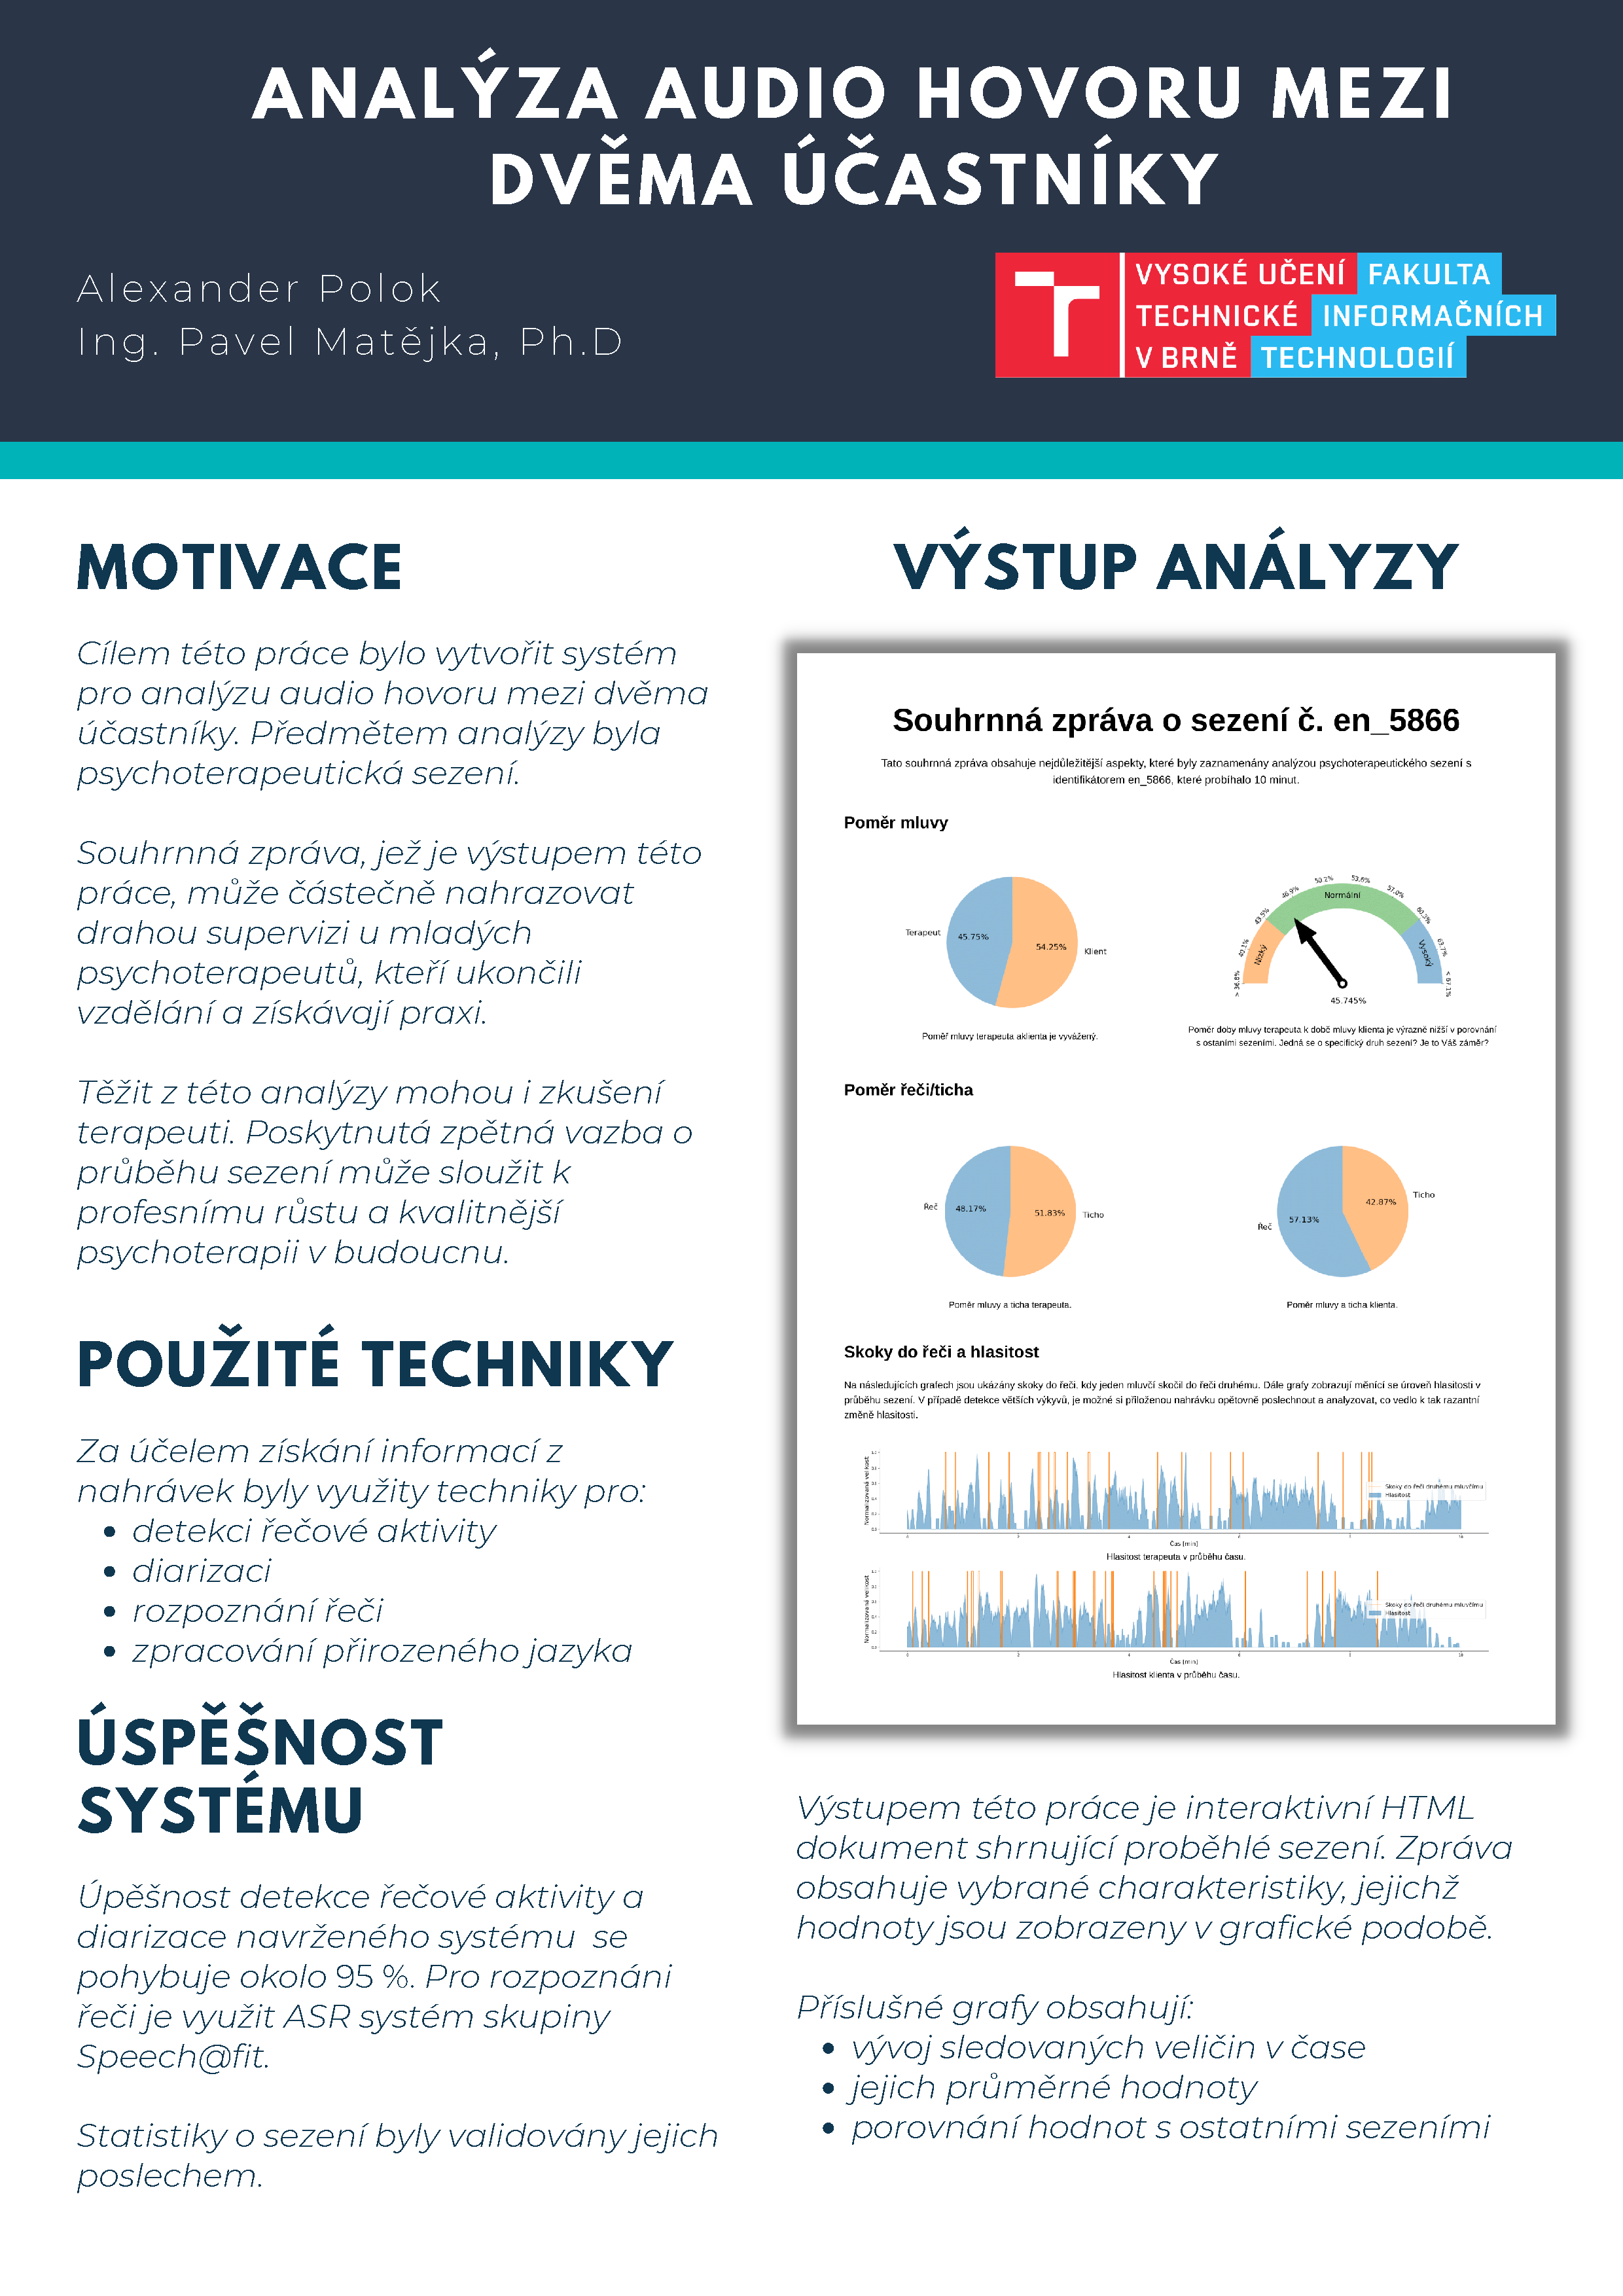
\includegraphics[height=0.67\textheight]{prilohy/plakat.pdf}
  \caption{Plakát prezentující navržený systém a jeho výstupy.}
  \label{fig:Poster}
\end{figure}

\chapter{Souhrnná zpráva}
\label{chap:Output_preview}
\begin{figure}[ht]
  \centering
  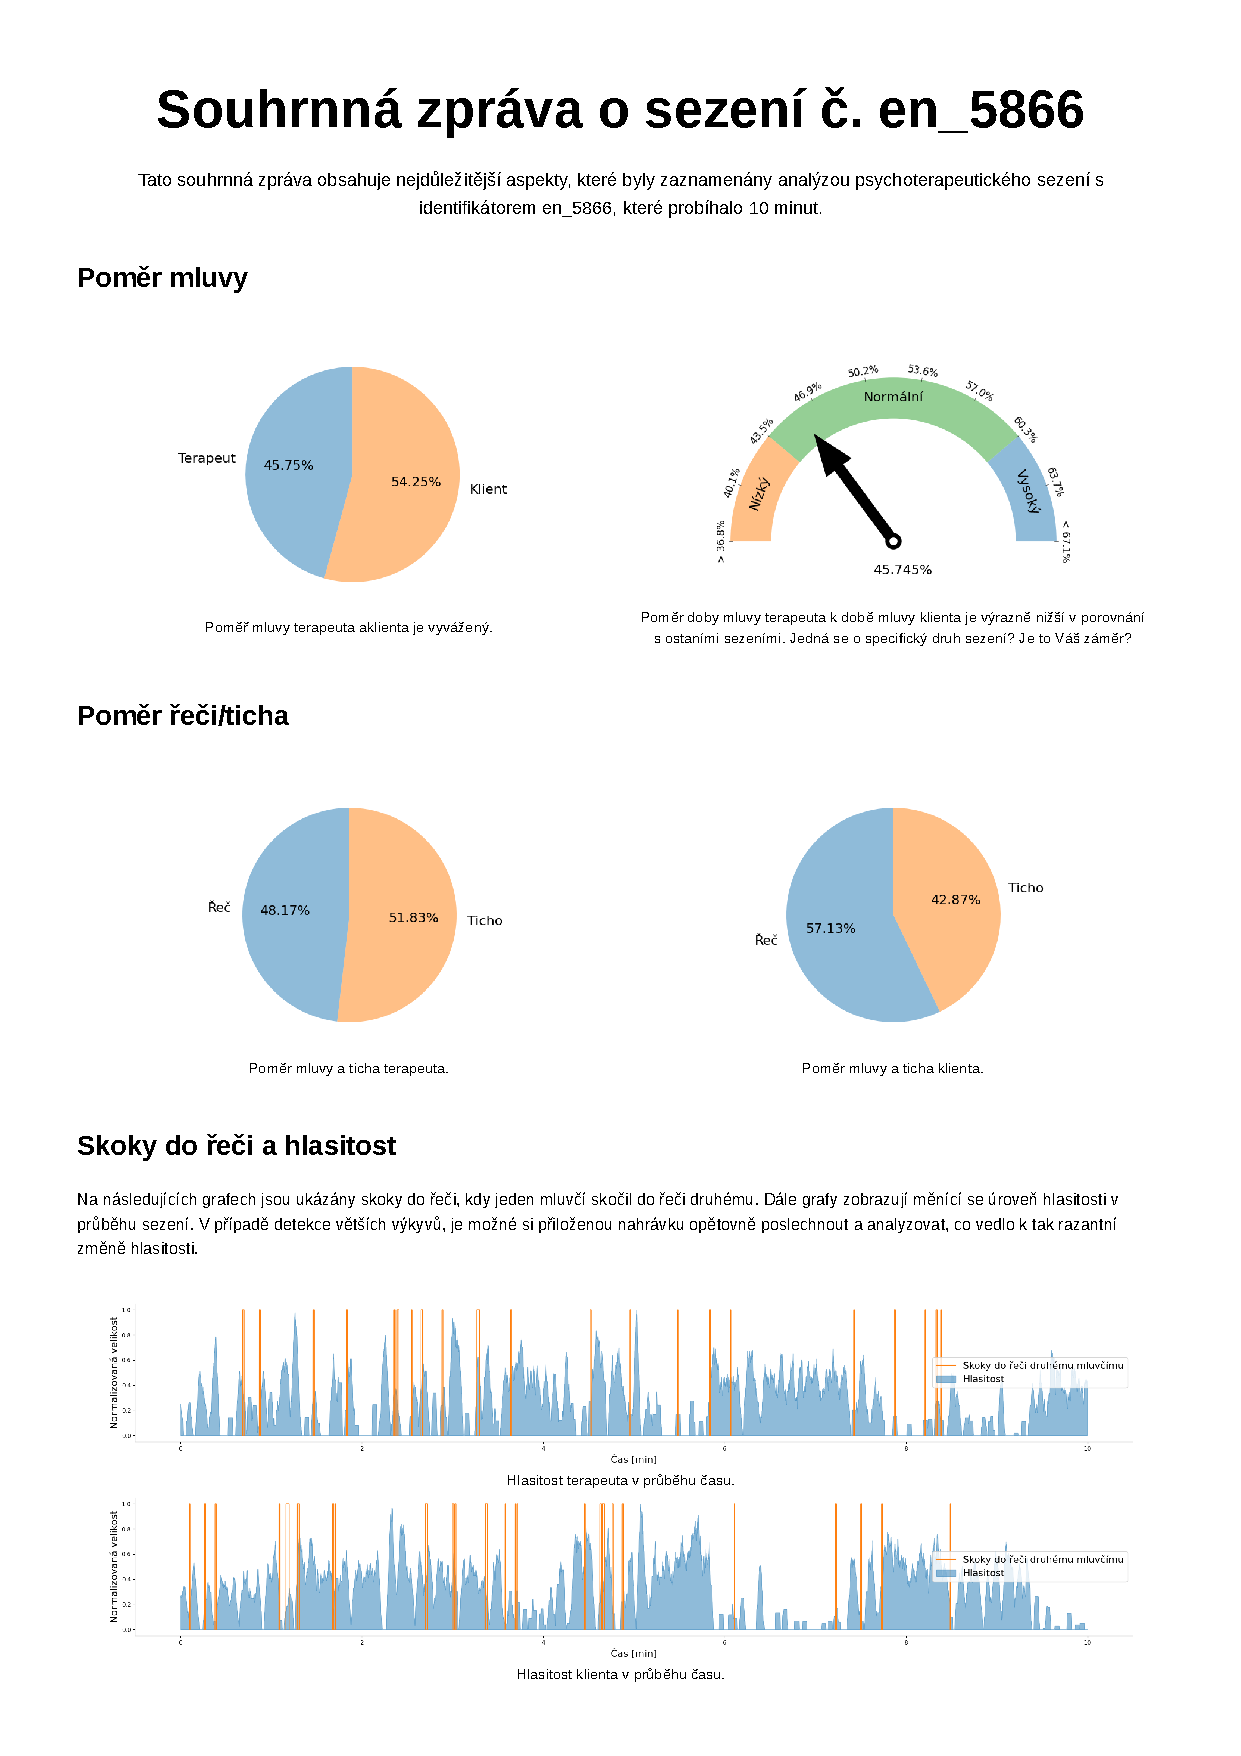
\includegraphics[height=0.64\textheight]{prilohy/output.pdf}
  \caption{Náhled části souhrnného dokumentu, který je automaticky vygenerován pro příslušná psychoterapeutická sezení.}
  \label{fig:Preview}
\end{figure}
  \fi
  
  % Kompilace po částech (viz výše, nutno odkomentovat)
  % Compilation piecewise (see above, it is necessary to uncomment it)
  %\subfile{projekt-30-prilohy-appendices}
  
\end{document}
